\documentclass[twoside]{book}

% Packages required by doxygen
\usepackage{fixltx2e}
\usepackage{calc}
\usepackage{doxygen}
\usepackage[export]{adjustbox} % also loads graphicx
\usepackage{graphicx}
\usepackage[utf8]{inputenc}
\usepackage{makeidx}
\usepackage{multicol}
\usepackage{multirow}
\PassOptionsToPackage{warn}{textcomp}
\usepackage{textcomp}
\usepackage[nointegrals]{wasysym}
\usepackage[table]{xcolor}

% NLS support packages
\usepackage[T2A]{fontenc}
\usepackage[russian]{babel}

% Font selection
\usepackage[T1]{fontenc}
\usepackage[scaled=.90]{helvet}
\usepackage{courier}
\usepackage{amssymb}
\usepackage{sectsty}
\renewcommand{\familydefault}{\sfdefault}
\allsectionsfont{%
  \fontseries{bc}\selectfont%
  \color{darkgray}%
}
\renewcommand{\DoxyLabelFont}{%
  \fontseries{bc}\selectfont%
  \color{darkgray}%
}
\newcommand{\+}{\discretionary{\mbox{\scriptsize$\hookleftarrow$}}{}{}}

% Page & text layout
\usepackage{geometry}
\geometry{%
  a4paper,%
  top=2.5cm,%
  bottom=2.5cm,%
  left=2.5cm,%
  right=2.5cm%
}
\tolerance=750
\hfuzz=15pt
\hbadness=750
\setlength{\emergencystretch}{15pt}
\setlength{\parindent}{0cm}
\setlength{\parskip}{3ex plus 2ex minus 2ex}
\makeatletter
\renewcommand{\paragraph}{%
  \@startsection{paragraph}{4}{0ex}{-1.0ex}{1.0ex}{%
    \normalfont\normalsize\bfseries\SS@parafont%
  }%
}
\renewcommand{\subparagraph}{%
  \@startsection{subparagraph}{5}{0ex}{-1.0ex}{1.0ex}{%
    \normalfont\normalsize\bfseries\SS@subparafont%
  }%
}
\makeatother

% Headers & footers
\usepackage{fancyhdr}
\pagestyle{fancyplain}
\fancyhead[LE]{\fancyplain{}{\bfseries\thepage}}
\fancyhead[CE]{\fancyplain{}{}}
\fancyhead[RE]{\fancyplain{}{\bfseries\leftmark}}
\fancyhead[LO]{\fancyplain{}{\bfseries\rightmark}}
\fancyhead[CO]{\fancyplain{}{}}
\fancyhead[RO]{\fancyplain{}{\bfseries\thepage}}
\fancyfoot[LE]{\fancyplain{}{}}
\fancyfoot[CE]{\fancyplain{}{}}
\fancyfoot[RE]{\fancyplain{}{\bfseries\scriptsize Создано системой Doxygen }}
\fancyfoot[LO]{\fancyplain{}{\bfseries\scriptsize Создано системой Doxygen }}
\fancyfoot[CO]{\fancyplain{}{}}
\fancyfoot[RO]{\fancyplain{}{}}
\renewcommand{\footrulewidth}{0.4pt}
\renewcommand{\chaptermark}[1]{%
  \markboth{#1}{}%
}
\renewcommand{\sectionmark}[1]{%
  \markright{\thesection\ #1}%
}

% Indices & bibliography
\usepackage{natbib}
\usepackage[titles]{tocloft}
\setcounter{tocdepth}{3}
\setcounter{secnumdepth}{5}
\makeindex

% Hyperlinks (required, but should be loaded last)
\usepackage{ifpdf}
\ifpdf
  \usepackage[pdftex,pagebackref=true]{hyperref}
\else
  \usepackage[ps2pdf,pagebackref=true]{hyperref}
\fi
\hypersetup{%
  colorlinks=true,%
  linkcolor=blue,%
  citecolor=blue,%
  unicode%
}

% Custom commands
\newcommand{\clearemptydoublepage}{%
  \newpage{\pagestyle{empty}\cleardoublepage}%
}

\usepackage{caption}
\captionsetup{labelsep=space,justification=centering,font={bf},singlelinecheck=off,skip=4pt,position=top}

%===== C O N T E N T S =====

\begin{document}

% Titlepage & ToC
\hypersetup{pageanchor=false,
             bookmarksnumbered=true,
             pdfencoding=unicode
            }
\pagenumbering{roman}
\begin{titlepage}
\vspace*{7cm}
\begin{center}%
{\Large Kpk }\\
\vspace*{1cm}
{\large Создано системой Doxygen 1.8.11}\\
\end{center}
\end{titlepage}
\clearemptydoublepage
\tableofcontents
\clearemptydoublepage
\pagenumbering{arabic}
\hypersetup{pageanchor=true}

%--- Begin generated contents ---
\chapter{Список задач}
\label{todo}
\hypertarget{todo}{}

\begin{DoxyRefList}
\item[\label{todo__todo000001}%
\hypertarget{todo__todo000001}{}%
Класс \hyperlink{classkpk_1_1core_1_1_person_service}{kpk\+:\+:core\+:\+:Person\+Service} ]Добавить работу с адресами 
\end{DoxyRefList}
\chapter{Алфавитный указатель пространств имен}
\section{Пространства имен}
Полный список пространств имен.\begin{DoxyCompactList}
\item\contentsline{section}{\hyperlink{namespacekpk}{kpk} }{\pageref{namespacekpk}}{}
\item\contentsline{section}{\hyperlink{namespacekpk_1_1core}{kpk\+::core} }{\pageref{namespacekpk_1_1core}}{}
\item\contentsline{section}{\hyperlink{namespacekpk_1_1data}{kpk\+::data} }{\pageref{namespacekpk_1_1data}}{}
\item\contentsline{section}{\hyperlink{namespacekpk_1_1exception}{kpk\+::exception} }{\pageref{namespacekpk_1_1exception}}{}
\item\contentsline{section}{\hyperlink{namespacekpk_1_1test}{kpk\+::test} }{\pageref{namespacekpk_1_1test}}{}
\end{DoxyCompactList}

\chapter{Иерархический список классов}
\section{Иерархия классов}
Иерархия классов.\begin{DoxyCompactList}
\item \contentsline{section}{kpk\+:\+:core\+:\+:Core\+Class}{\pageref{classkpk_1_1core_1_1_core_class}}{}
\item \contentsline{section}{kpk\+:\+:core\+:\+:Db\+Service}{\pageref{classkpk_1_1core_1_1_db_service}}{}
\item exception\begin{DoxyCompactList}
\item \contentsline{section}{kpk\+:\+:exception\+:\+:Already\+Member\+Exception}{\pageref{classkpk_1_1exception_1_1_already_member_exception}}{}
\item \contentsline{section}{kpk\+:\+:exception\+:\+:Not\+A\+Member\+Exception}{\pageref{classkpk_1_1exception_1_1_not_a_member_exception}}{}
\end{DoxyCompactList}
\item \contentsline{section}{kpk\+:\+:data\+:\+:Is\+Deleted}{\pageref{classkpk_1_1data_1_1_is_deleted}}{}
\begin{DoxyCompactList}
\item \contentsline{section}{kpk\+:\+:data\+:\+:Loan}{\pageref{classkpk_1_1data_1_1_loan}}{}
\item \contentsline{section}{kpk\+:\+:data\+:\+:Loan\+Oper}{\pageref{classkpk_1_1data_1_1_loan_oper}}{}
\end{DoxyCompactList}
\item \contentsline{section}{kpk\+:\+:data\+:\+:Loan\+Oper\+Value}{\pageref{classkpk_1_1data_1_1_loan_oper_value}}{}
\item \contentsline{section}{kpk\+:\+:core\+:\+:Loan\+Service}{\pageref{classkpk_1_1core_1_1_loan_service}}{}
\item \contentsline{section}{kpk\+:\+:data\+:\+:Loan\+Type}{\pageref{classkpk_1_1data_1_1_loan_type}}{}
\item \contentsline{section}{kpk\+:\+:data\+:\+:Member}{\pageref{classkpk_1_1data_1_1_member}}{}
\item \contentsline{section}{kpk\+:\+:data\+:\+:Name}{\pageref{classkpk_1_1data_1_1_name}}{}
\item \contentsline{section}{kpk\+:\+:data\+:\+:Passport}{\pageref{classkpk_1_1data_1_1_passport}}{}
\item \contentsline{section}{kpk\+:\+:data\+:\+:Person}{\pageref{classkpk_1_1data_1_1_person}}{}
\item \contentsline{section}{kpk\+:\+:core\+:\+:Person\+Service}{\pageref{classkpk_1_1core_1_1_person_service}}{}
\item Q\+Object\begin{DoxyCompactList}
\item \contentsline{section}{data\+Test}{\pageref{classdata_test}}{}
\item \contentsline{section}{kpk\+:\+:test\+:\+:Kpk\+Core\+Test}{\pageref{classkpk_1_1test_1_1_kpk_core_test}}{}
\item \contentsline{section}{kpk\+:\+:test\+:\+:kpk\+Data\+Test}{\pageref{classkpk_1_1test_1_1kpk_data_test}}{}
\end{DoxyCompactList}
\end{DoxyCompactList}

\chapter{Алфавитный указатель классов}
\section{Классы}
Классы с их кратким описанием.\begin{DoxyCompactList}
\item\contentsline{section}{\hyperlink{structkpk_1_1exception_1_1_already_member_exception}{kpk\+::exception\+::\+Already\+Member\+Exception} }{\pageref{structkpk_1_1exception_1_1_already_member_exception}}{}
\item\contentsline{section}{\hyperlink{classkpk_1_1core_1_1_core_class}{kpk\+::core\+::\+Core\+Class} \\*Класс Ядра }{\pageref{classkpk_1_1core_1_1_core_class}}{}
\item\contentsline{section}{\hyperlink{classdata_test}{data\+Test} }{\pageref{classdata_test}}{}
\item\contentsline{section}{\hyperlink{classkpk_1_1core_1_1_db_service}{kpk\+::core\+::\+Db\+Service} \\*Служба управления базой данных }{\pageref{classkpk_1_1core_1_1_db_service}}{}
\item\contentsline{section}{\hyperlink{classkpk_1_1test_1_1_kpk_core_test}{kpk\+::test\+::\+Kpk\+Core\+Test} }{\pageref{classkpk_1_1test_1_1_kpk_core_test}}{}
\item\contentsline{section}{\hyperlink{classkpk_1_1test_1_1kpk_data_test}{kpk\+::test\+::kpk\+Data\+Test} }{\pageref{classkpk_1_1test_1_1kpk_data_test}}{}
\item\contentsline{section}{\hyperlink{classkpk_1_1data_1_1_loan}{kpk\+::data\+::\+Loan} \\*Займ }{\pageref{classkpk_1_1data_1_1_loan}}{}
\item\contentsline{section}{\hyperlink{classkpk_1_1data_1_1_loan_oper}{kpk\+::data\+::\+Loan\+Oper} \\*Операция по займу }{\pageref{classkpk_1_1data_1_1_loan_oper}}{}
\item\contentsline{section}{\hyperlink{classkpk_1_1data_1_1_loan_oper_value}{kpk\+::data\+::\+Loan\+Oper\+Value} \\*Данные операции по займу }{\pageref{classkpk_1_1data_1_1_loan_oper_value}}{}
\item\contentsline{section}{\hyperlink{classkpk_1_1core_1_1_loan_service}{kpk\+::core\+::\+Loan\+Service} }{\pageref{classkpk_1_1core_1_1_loan_service}}{}
\item\contentsline{section}{\hyperlink{classkpk_1_1data_1_1_member}{kpk\+::data\+::\+Member} \\*Пайщик }{\pageref{classkpk_1_1data_1_1_member}}{}
\item\contentsline{section}{\hyperlink{classkpk_1_1data_1_1_name}{kpk\+::data\+::\+Name} \\*Полное имя }{\pageref{classkpk_1_1data_1_1_name}}{}
\item\contentsline{section}{\hyperlink{structkpk_1_1exception_1_1_not_a_member_exception}{kpk\+::exception\+::\+Not\+A\+Member\+Exception} }{\pageref{structkpk_1_1exception_1_1_not_a_member_exception}}{}
\item\contentsline{section}{\hyperlink{classkpk_1_1data_1_1_passport}{kpk\+::data\+::\+Passport} \\*Паспортные данные }{\pageref{classkpk_1_1data_1_1_passport}}{}
\item\contentsline{section}{\hyperlink{classkpk_1_1data_1_1_person}{kpk\+::data\+::\+Person} \\*Личные данные }{\pageref{classkpk_1_1data_1_1_person}}{}
\item\contentsline{section}{\hyperlink{classkpk_1_1core_1_1_person_service}{kpk\+::core\+::\+Person\+Service} \\*Служба по управлению личными данными }{\pageref{classkpk_1_1core_1_1_person_service}}{}
\end{DoxyCompactList}

\chapter{Список файлов}
\section{Файлы}
Полный список файлов.\begin{DoxyCompactList}
\item\contentsline{section}{kpk-\/core-\/test/\hyperlink{tst___kpk_core_test_8cpp}{tst\+\_\+\+Kpk\+Core\+Test.\+cpp} }{\pageref{tst___kpk_core_test_8cpp}}{}
\item\contentsline{section}{kpk-\/core/\hyperlink{_core_8cpp}{Core.\+cpp} }{\pageref{_core_8cpp}}{}
\item\contentsline{section}{kpk-\/core/\hyperlink{_core_8h}{Core.\+h} }{\pageref{_core_8h}}{}
\item\contentsline{section}{kpk-\/core/\hyperlink{core__global_8h}{core\+\_\+global.\+h} }{\pageref{core__global_8h}}{}
\item\contentsline{section}{kpk-\/core/\hyperlink{_db_service_8cpp}{Db\+Service.\+cpp} }{\pageref{_db_service_8cpp}}{}
\item\contentsline{section}{kpk-\/core/\hyperlink{_db_service_8h}{Db\+Service.\+h} }{\pageref{_db_service_8h}}{}
\item\contentsline{section}{kpk-\/core/\hyperlink{_exceptions_8h}{Exceptions.\+h} \\*Исключения }{\pageref{_exceptions_8h}}{}
\item\contentsline{section}{kpk-\/core/\hyperlink{_loan_service_8h}{Loan\+Service.\+h} }{\pageref{_loan_service_8h}}{}
\item\contentsline{section}{kpk-\/core/\hyperlink{_person_service_8cpp}{Person\+Service.\+cpp} }{\pageref{_person_service_8cpp}}{}
\item\contentsline{section}{kpk-\/core/\hyperlink{_person_service_8h}{Person\+Service.\+h} }{\pageref{_person_service_8h}}{}
\item\contentsline{section}{kpk-\/data-\/test/\hyperlink{tst__data_test_8cpp}{tst\+\_\+data\+Test.\+cpp} }{\pageref{tst__data_test_8cpp}}{}
\item\contentsline{section}{kpk-\/data-\/test/\hyperlink{tst__kpk_data_test_8cpp}{tst\+\_\+kpk\+Data\+Test.\+cpp} }{\pageref{tst__kpk_data_test_8cpp}}{}
\item\contentsline{section}{kpk-\/data/\hyperlink{data__global_8h}{data\+\_\+global.\+h} \\*Необходимые директивы препроцессора }{\pageref{data__global_8h}}{}
\item\contentsline{section}{kpk-\/data/\hyperlink{_is_deleted_8cpp}{Is\+Deleted.\+cpp} }{\pageref{_is_deleted_8cpp}}{}
\item\contentsline{section}{kpk-\/data/\hyperlink{_is_deleted_8h}{Is\+Deleted.\+h} }{\pageref{_is_deleted_8h}}{}
\item\contentsline{section}{kpk-\/data/\hyperlink{_loan_8cpp}{Loan.\+cpp} }{\pageref{_loan_8cpp}}{}
\item\contentsline{section}{kpk-\/data/\hyperlink{_loan_8h}{Loan.\+h} }{\pageref{_loan_8h}}{}
\item\contentsline{section}{kpk-\/data/\hyperlink{_loan_oper_8cpp}{Loan\+Oper.\+cpp} }{\pageref{_loan_oper_8cpp}}{}
\item\contentsline{section}{kpk-\/data/\hyperlink{_loan_oper_8h}{Loan\+Oper.\+h} }{\pageref{_loan_oper_8h}}{}
\item\contentsline{section}{kpk-\/data/\hyperlink{_loan_oper_value_8cpp}{Loan\+Oper\+Value.\+cpp} }{\pageref{_loan_oper_value_8cpp}}{}
\item\contentsline{section}{kpk-\/data/\hyperlink{_loan_oper_value_8h}{Loan\+Oper\+Value.\+h} }{\pageref{_loan_oper_value_8h}}{}
\item\contentsline{section}{kpk-\/data/\hyperlink{_loan_type_8cpp}{Loan\+Type.\+cpp} }{\pageref{_loan_type_8cpp}}{}
\item\contentsline{section}{kpk-\/data/\hyperlink{_loan_type_8h}{Loan\+Type.\+h} }{\pageref{_loan_type_8h}}{}
\item\contentsline{section}{kpk-\/data/\hyperlink{_member_8cpp}{Member.\+cpp} }{\pageref{_member_8cpp}}{}
\item\contentsline{section}{kpk-\/data/\hyperlink{_member_8h}{Member.\+h} }{\pageref{_member_8h}}{}
\item\contentsline{section}{kpk-\/data/\hyperlink{_name_8cpp}{Name.\+cpp} }{\pageref{_name_8cpp}}{}
\item\contentsline{section}{kpk-\/data/\hyperlink{_name_8h}{Name.\+h} }{\pageref{_name_8h}}{}
\item\contentsline{section}{kpk-\/data/\hyperlink{_passport_8cpp}{Passport.\+cpp} }{\pageref{_passport_8cpp}}{}
\item\contentsline{section}{kpk-\/data/\hyperlink{_passport_8h}{Passport.\+h} }{\pageref{_passport_8h}}{}
\item\contentsline{section}{kpk-\/data/\hyperlink{_person_8cpp}{Person.\+cpp} }{\pageref{_person_8cpp}}{}
\item\contentsline{section}{kpk-\/data/\hyperlink{_person_8h}{Person.\+h} }{\pageref{_person_8h}}{}
\item\contentsline{section}{kpk-\/test-\/console/\hyperlink{kpk-test-console_2main_8cpp}{main.\+cpp} }{\pageref{kpk-test-console_2main_8cpp}}{}
\item\contentsline{section}{kpk-\/test-\/quick/\hyperlink{kpk-test-quick_2main_8cpp}{main.\+cpp} }{\pageref{kpk-test-quick_2main_8cpp}}{}
\end{DoxyCompactList}

\chapter{Пространства имен}
\hypertarget{namespacekpk}{}\section{Пространство имен kpk}
\label{namespacekpk}\index{kpk@{kpk}}
\subsection*{Пространства имен}
\begin{DoxyCompactItemize}
\item 
 \hyperlink{namespacekpk_1_1core}{core}
\item 
 \hyperlink{namespacekpk_1_1data}{data}
\item 
 \hyperlink{namespacekpk_1_1exception}{exception}
\item 
 \hyperlink{namespacekpk_1_1test}{test}
\end{DoxyCompactItemize}

\hypertarget{namespacekpk_1_1core}{}\section{Пространство имен kpk\+:\+:core}
\label{namespacekpk_1_1core}\index{kpk\+::core@{kpk\+::core}}
\subsection*{Классы}
\begin{DoxyCompactItemize}
\item 
class \hyperlink{classkpk_1_1core_1_1_core_class}{Core\+Class}
\begin{DoxyCompactList}\small\item\em Класс Ядра \end{DoxyCompactList}\item 
class \hyperlink{classkpk_1_1core_1_1_db_service}{Db\+Service}
\begin{DoxyCompactList}\small\item\em Служба управления базой данных \end{DoxyCompactList}\item 
class \hyperlink{classkpk_1_1core_1_1_loan_service}{Loan\+Service}
\item 
class \hyperlink{classkpk_1_1core_1_1_person_service}{Person\+Service}
\begin{DoxyCompactList}\small\item\em Служба по управлению личными данными \end{DoxyCompactList}\end{DoxyCompactItemize}
\subsection*{Определения типов}
\begin{DoxyCompactItemize}
\item 
typedef Q\+Shared\+Pointer$<$ odb\+::database $>$ \hyperlink{namespacekpk_1_1core_a57462cfcc109ed2afcc118d0668710cf}{Db\+Ptr}
\item 
typedef Q\+Shared\+Pointer$<$ odb\+::transaction $>$ \hyperlink{namespacekpk_1_1core_a3bd2bbeaff3894d4ee696d6fae548f3f}{Tr\+Ptr}
\item 
typedef Q\+Shared\+Pointer$<$ \hyperlink{classkpk_1_1data_1_1_person}{data\+::\+Person} $>$ \hyperlink{namespacekpk_1_1core_a4a1c110098ffdfb42bdcba45c4d9a7fe}{Person\+Ptr}
\begin{DoxyCompactList}\small\item\em Person\+Ptr Указатель на личные данные \end{DoxyCompactList}\item 
typedef Q\+Shared\+Pointer$<$ \hyperlink{classkpk_1_1data_1_1_member}{data\+::\+Member} $>$ \hyperlink{namespacekpk_1_1core_aca962f7fa9cb72f79643863d3634f7b9}{Member\+Ptr}
\begin{DoxyCompactList}\small\item\em Указатель на запись членства \end{DoxyCompactList}\end{DoxyCompactItemize}


\subsection{Типы}
\index{kpk\+::core@{kpk\+::core}!Db\+Ptr@{Db\+Ptr}}
\index{Db\+Ptr@{Db\+Ptr}!kpk\+::core@{kpk\+::core}}
\subsubsection[{\texorpdfstring{Db\+Ptr}{DbPtr}}]{\setlength{\rightskip}{0pt plus 5cm}typedef Q\+Shared\+Pointer$<$odb\+::database$>$ {\bf kpk\+::core\+::\+Db\+Ptr}}\hypertarget{namespacekpk_1_1core_a57462cfcc109ed2afcc118d0668710cf}{}\label{namespacekpk_1_1core_a57462cfcc109ed2afcc118d0668710cf}


См. определение в файле Db\+Service.\+h строка 13

\index{kpk\+::core@{kpk\+::core}!Member\+Ptr@{Member\+Ptr}}
\index{Member\+Ptr@{Member\+Ptr}!kpk\+::core@{kpk\+::core}}
\subsubsection[{\texorpdfstring{Member\+Ptr}{MemberPtr}}]{\setlength{\rightskip}{0pt plus 5cm}typedef Q\+Shared\+Pointer$<${\bf data\+::\+Member}$>$ {\bf kpk\+::core\+::\+Member\+Ptr}}\hypertarget{namespacekpk_1_1core_aca962f7fa9cb72f79643863d3634f7b9}{}\label{namespacekpk_1_1core_aca962f7fa9cb72f79643863d3634f7b9}


Указатель на запись членства 



См. определение в файле Person\+Service.\+h строка 20

\index{kpk\+::core@{kpk\+::core}!Person\+Ptr@{Person\+Ptr}}
\index{Person\+Ptr@{Person\+Ptr}!kpk\+::core@{kpk\+::core}}
\subsubsection[{\texorpdfstring{Person\+Ptr}{PersonPtr}}]{\setlength{\rightskip}{0pt plus 5cm}typedef Q\+Shared\+Pointer$<${\bf data\+::\+Person}$>$ {\bf kpk\+::core\+::\+Person\+Ptr}}\hypertarget{namespacekpk_1_1core_a4a1c110098ffdfb42bdcba45c4d9a7fe}{}\label{namespacekpk_1_1core_a4a1c110098ffdfb42bdcba45c4d9a7fe}


Person\+Ptr Указатель на личные данные 



См. определение в файле Person\+Service.\+h строка 16

\index{kpk\+::core@{kpk\+::core}!Tr\+Ptr@{Tr\+Ptr}}
\index{Tr\+Ptr@{Tr\+Ptr}!kpk\+::core@{kpk\+::core}}
\subsubsection[{\texorpdfstring{Tr\+Ptr}{TrPtr}}]{\setlength{\rightskip}{0pt plus 5cm}typedef Q\+Shared\+Pointer$<$odb\+::transaction$>$ {\bf kpk\+::core\+::\+Tr\+Ptr}}\hypertarget{namespacekpk_1_1core_a3bd2bbeaff3894d4ee696d6fae548f3f}{}\label{namespacekpk_1_1core_a3bd2bbeaff3894d4ee696d6fae548f3f}


См. определение в файле Db\+Service.\+h строка 14


\hypertarget{namespacekpk_1_1data}{}\section{Пространство имен kpk\+:\+:data}
\label{namespacekpk_1_1data}\index{kpk\+::data@{kpk\+::data}}
\subsection*{Классы}
\begin{DoxyCompactItemize}
\item 
class \hyperlink{classkpk_1_1data_1_1_loan}{Loan}
\begin{DoxyCompactList}\small\item\em Займ \end{DoxyCompactList}\item 
class \hyperlink{classkpk_1_1data_1_1_loan_oper}{Loan\+Oper}
\begin{DoxyCompactList}\small\item\em Операция по займу \end{DoxyCompactList}\item 
class \hyperlink{classkpk_1_1data_1_1_loan_oper_value}{Loan\+Oper\+Value}
\begin{DoxyCompactList}\small\item\em Данные операции по займу \end{DoxyCompactList}\item 
class \hyperlink{classkpk_1_1data_1_1_loan_type}{Loan\+Type}
\begin{DoxyCompactList}\small\item\em Вид займа \end{DoxyCompactList}\item 
class \hyperlink{classkpk_1_1data_1_1_member}{Member}
\begin{DoxyCompactList}\small\item\em Пайщик \end{DoxyCompactList}\item 
class \hyperlink{classkpk_1_1data_1_1_name}{Name}
\begin{DoxyCompactList}\small\item\em Полное имя \end{DoxyCompactList}\item 
class \hyperlink{classkpk_1_1data_1_1_passport}{Passport}
\begin{DoxyCompactList}\small\item\em Паспортные данные \end{DoxyCompactList}\item 
class \hyperlink{classkpk_1_1data_1_1_person}{Person}
\begin{DoxyCompactList}\small\item\em Человек \end{DoxyCompactList}\end{DoxyCompactItemize}
\subsection*{Перечисления}
\begin{DoxyCompactItemize}
\item 
enum \hyperlink{namespacekpk_1_1data_a16790bc647a6788cab282e185ee28998}{Exit\+Reason} \{ \hyperlink{namespacekpk_1_1data_a16790bc647a6788cab282e185ee28998aa134c23d38704d99db23ef993830c24a}{E\+R\+\_\+\+N\+O\+NE}, 
\hyperlink{namespacekpk_1_1data_a16790bc647a6788cab282e185ee28998a72cce9ef1a1a013bca99ece41bc13431}{E\+R\+\_\+\+E\+X\+IT}, 
\hyperlink{namespacekpk_1_1data_a16790bc647a6788cab282e185ee28998a8cfb19daa38668796673a2ce7ce15f24}{E\+R\+\_\+\+K\+I\+CK}, 
\hyperlink{namespacekpk_1_1data_a16790bc647a6788cab282e185ee28998a2063b2e237a0013b06ed6eedc4b8bc48}{E\+R\+\_\+\+D\+E\+A\+TH}
 \}\begin{DoxyCompactList}\small\item\em Причина выхода \end{DoxyCompactList}
\end{DoxyCompactItemize}


\subsection{Перечисления}
\index{kpk\+::data@{kpk\+::data}!Exit\+Reason@{Exit\+Reason}}
\index{Exit\+Reason@{Exit\+Reason}!kpk\+::data@{kpk\+::data}}
\subsubsection[{\texorpdfstring{Exit\+Reason}{ExitReason}}]{\setlength{\rightskip}{0pt plus 5cm}enum {\bf kpk\+::data\+::\+Exit\+Reason}}\hypertarget{namespacekpk_1_1data_a16790bc647a6788cab282e185ee28998}{}\label{namespacekpk_1_1data_a16790bc647a6788cab282e185ee28998}


Причина выхода 

\begin{Desc}
\item[Элементы перечислений]\par
\begin{description}
\index{E\+R\+\_\+\+N\+O\+NE@{E\+R\+\_\+\+N\+O\+NE}!kpk\+::data@{kpk\+::data}}\index{kpk\+::data@{kpk\+::data}!E\+R\+\_\+\+N\+O\+NE@{E\+R\+\_\+\+N\+O\+NE}}\item[{\em 
E\+R\+\_\+\+N\+O\+NE\hypertarget{namespacekpk_1_1data_a16790bc647a6788cab282e185ee28998aa134c23d38704d99db23ef993830c24a}{}\label{namespacekpk_1_1data_a16790bc647a6788cab282e185ee28998aa134c23d38704d99db23ef993830c24a}
}]Не вышел \index{E\+R\+\_\+\+E\+X\+IT@{E\+R\+\_\+\+E\+X\+IT}!kpk\+::data@{kpk\+::data}}\index{kpk\+::data@{kpk\+::data}!E\+R\+\_\+\+E\+X\+IT@{E\+R\+\_\+\+E\+X\+IT}}\item[{\em 
E\+R\+\_\+\+E\+X\+IT\hypertarget{namespacekpk_1_1data_a16790bc647a6788cab282e185ee28998a72cce9ef1a1a013bca99ece41bc13431}{}\label{namespacekpk_1_1data_a16790bc647a6788cab282e185ee28998a72cce9ef1a1a013bca99ece41bc13431}
}]Вышел добровольно \index{E\+R\+\_\+\+K\+I\+CK@{E\+R\+\_\+\+K\+I\+CK}!kpk\+::data@{kpk\+::data}}\index{kpk\+::data@{kpk\+::data}!E\+R\+\_\+\+K\+I\+CK@{E\+R\+\_\+\+K\+I\+CK}}\item[{\em 
E\+R\+\_\+\+K\+I\+CK\hypertarget{namespacekpk_1_1data_a16790bc647a6788cab282e185ee28998a8cfb19daa38668796673a2ce7ce15f24}{}\label{namespacekpk_1_1data_a16790bc647a6788cab282e185ee28998a8cfb19daa38668796673a2ce7ce15f24}
}]Исключен \index{E\+R\+\_\+\+D\+E\+A\+TH@{E\+R\+\_\+\+D\+E\+A\+TH}!kpk\+::data@{kpk\+::data}}\index{kpk\+::data@{kpk\+::data}!E\+R\+\_\+\+D\+E\+A\+TH@{E\+R\+\_\+\+D\+E\+A\+TH}}\item[{\em 
E\+R\+\_\+\+D\+E\+A\+TH\hypertarget{namespacekpk_1_1data_a16790bc647a6788cab282e185ee28998a2063b2e237a0013b06ed6eedc4b8bc48}{}\label{namespacekpk_1_1data_a16790bc647a6788cab282e185ee28998a2063b2e237a0013b06ed6eedc4b8bc48}
}]Умер \end{description}
\end{Desc}


См. определение в файле Member.\+h строка 17


\hypertarget{namespacekpk_1_1exception}{}\section{Пространство имен kpk\+:\+:exception}
\label{namespacekpk_1_1exception}\index{kpk\+::exception@{kpk\+::exception}}
\subsection*{Классы}
\begin{DoxyCompactItemize}
\item 
struct \hyperlink{structkpk_1_1exception_1_1_already_member_exception}{Already\+Member\+Exception}
\item 
struct \hyperlink{structkpk_1_1exception_1_1_not_a_member_exception}{Not\+A\+Member\+Exception}
\end{DoxyCompactItemize}

\hypertarget{namespacekpk_1_1test}{}\section{Пространство имен kpk\+:\+:test}
\label{namespacekpk_1_1test}\index{kpk\+::test@{kpk\+::test}}
\subsection*{Классы}
\begin{DoxyCompactItemize}
\item 
class \hyperlink{classkpk_1_1test_1_1_kpk_core_test}{Kpk\+Core\+Test}
\item 
class \hyperlink{classkpk_1_1test_1_1kpk_data_test}{kpk\+Data\+Test}
\end{DoxyCompactItemize}

\chapter{Классы}
\input{classkpk_1_1exception_1_1_already_member_exception}
\hypertarget{classkpk_1_1core_1_1_core_class}{}\section{Класс kpk\+:\+:core\+:\+:Core\+Class}
\label{classkpk_1_1core_1_1_core_class}\index{kpk\+::core\+::\+Core\+Class@{kpk\+::core\+::\+Core\+Class}}


Класс Ядра  




{\ttfamily \#include $<$Core.\+h$>$}

\subsection*{Открытые члены}
\begin{DoxyCompactItemize}
\item 
\hyperlink{classkpk_1_1core_1_1_core_class_a5dc08a07fb3d8e84da07623d7739261a}{Core\+Class} ()
\item 
Q\+Shared\+Pointer$<$ \hyperlink{classkpk_1_1core_1_1_db_service}{Db\+Service} $>$ \& \hyperlink{classkpk_1_1core_1_1_core_class_a98a1fe99a1e3a6e99b8539995b539e43}{db\+Service} ()
\begin{DoxyCompactList}\small\item\em Служба управления базой данных \end{DoxyCompactList}\item 
\hyperlink{namespacekpk_1_1core_a57462cfcc109ed2afcc118d0668710cf}{Db\+Ptr} \hyperlink{classkpk_1_1core_1_1_core_class_aeb0cc8cb53c4ab4dc945226bd4f349d2}{db} ()
\begin{DoxyCompactList}\small\item\em Основная база данных \end{DoxyCompactList}\item 
Q\+Shared\+Pointer$<$ \hyperlink{classkpk_1_1core_1_1_person_service}{Person\+Service} $>$ \& \hyperlink{classkpk_1_1core_1_1_core_class_a5de72b91f0c71183286d643dc3fca8b7}{person} ()
\begin{DoxyCompactList}\small\item\em Служба управления личными данными \end{DoxyCompactList}\item 
void \hyperlink{classkpk_1_1core_1_1_core_class_addd4edd20d222119a0ddc384ee73cfb9}{begin} ()
\begin{DoxyCompactList}\small\item\em Начать транзакцию в основной базе \end{DoxyCompactList}\item 
void \hyperlink{classkpk_1_1core_1_1_core_class_a4b9e63dd9e488616d4a70a6b3c8a929c}{commit} ()
\begin{DoxyCompactList}\small\item\em Фиксировать транзакцию в основной базе \end{DoxyCompactList}\item 
void \hyperlink{classkpk_1_1core_1_1_core_class_a6e64f22a4b5d786e3172b13a671971af}{rollback} ()
\begin{DoxyCompactList}\small\item\em Отменить транзакцию в основной базе \end{DoxyCompactList}\end{DoxyCompactItemize}


\subsection{Подробное описание}
Класс Ядра 

Все службы собранные в кучу 

См. определение в файле Core.\+h строка 18



\subsection{Конструктор(ы)}
\index{kpk\+::core\+::\+Core\+Class@{kpk\+::core\+::\+Core\+Class}!Core\+Class@{Core\+Class}}
\index{Core\+Class@{Core\+Class}!kpk\+::core\+::\+Core\+Class@{kpk\+::core\+::\+Core\+Class}}
\subsubsection[{\texorpdfstring{Core\+Class()}{CoreClass()}}]{\setlength{\rightskip}{0pt plus 5cm}kpk\+::core\+::\+Core\+Class\+::\+Core\+Class (
\begin{DoxyParamCaption}
{}
\end{DoxyParamCaption}
)}\hypertarget{classkpk_1_1core_1_1_core_class_a5dc08a07fb3d8e84da07623d7739261a}{}\label{classkpk_1_1core_1_1_core_class_a5dc08a07fb3d8e84da07623d7739261a}


См. определение в файле Core.\+cpp строка 6



\subsection{Методы}
\index{kpk\+::core\+::\+Core\+Class@{kpk\+::core\+::\+Core\+Class}!begin@{begin}}
\index{begin@{begin}!kpk\+::core\+::\+Core\+Class@{kpk\+::core\+::\+Core\+Class}}
\subsubsection[{\texorpdfstring{begin()}{begin()}}]{\setlength{\rightskip}{0pt plus 5cm}void kpk\+::core\+::\+Core\+Class\+::begin (
\begin{DoxyParamCaption}
{}
\end{DoxyParamCaption}
)}\hypertarget{classkpk_1_1core_1_1_core_class_addd4edd20d222119a0ddc384ee73cfb9}{}\label{classkpk_1_1core_1_1_core_class_addd4edd20d222119a0ddc384ee73cfb9}


Начать транзакцию в основной базе 



См. определение в файле Core.\+cpp строка 27

\index{kpk\+::core\+::\+Core\+Class@{kpk\+::core\+::\+Core\+Class}!commit@{commit}}
\index{commit@{commit}!kpk\+::core\+::\+Core\+Class@{kpk\+::core\+::\+Core\+Class}}
\subsubsection[{\texorpdfstring{commit()}{commit()}}]{\setlength{\rightskip}{0pt plus 5cm}void kpk\+::core\+::\+Core\+Class\+::commit (
\begin{DoxyParamCaption}
{}
\end{DoxyParamCaption}
)}\hypertarget{classkpk_1_1core_1_1_core_class_a4b9e63dd9e488616d4a70a6b3c8a929c}{}\label{classkpk_1_1core_1_1_core_class_a4b9e63dd9e488616d4a70a6b3c8a929c}


Фиксировать транзакцию в основной базе 



См. определение в файле Core.\+cpp строка 32

\index{kpk\+::core\+::\+Core\+Class@{kpk\+::core\+::\+Core\+Class}!db@{db}}
\index{db@{db}!kpk\+::core\+::\+Core\+Class@{kpk\+::core\+::\+Core\+Class}}
\subsubsection[{\texorpdfstring{db()}{db()}}]{\setlength{\rightskip}{0pt plus 5cm}{\bf Db\+Ptr} kpk\+::core\+::\+Core\+Class\+::db (
\begin{DoxyParamCaption}
{}
\end{DoxyParamCaption}
)}\hypertarget{classkpk_1_1core_1_1_core_class_aeb0cc8cb53c4ab4dc945226bd4f349d2}{}\label{classkpk_1_1core_1_1_core_class_aeb0cc8cb53c4ab4dc945226bd4f349d2}


Основная база данных 

\begin{DoxyReturn}{Возвращает}
Указатель на базу данных 
\end{DoxyReturn}


См. определение в файле Core.\+cpp строка 17

\index{kpk\+::core\+::\+Core\+Class@{kpk\+::core\+::\+Core\+Class}!db\+Service@{db\+Service}}
\index{db\+Service@{db\+Service}!kpk\+::core\+::\+Core\+Class@{kpk\+::core\+::\+Core\+Class}}
\subsubsection[{\texorpdfstring{db\+Service()}{dbService()}}]{\setlength{\rightskip}{0pt plus 5cm}Q\+Shared\+Pointer$<$ {\bf Db\+Service} $>$ \& kpk\+::core\+::\+Core\+Class\+::db\+Service (
\begin{DoxyParamCaption}
{}
\end{DoxyParamCaption}
)}\hypertarget{classkpk_1_1core_1_1_core_class_a98a1fe99a1e3a6e99b8539995b539e43}{}\label{classkpk_1_1core_1_1_core_class_a98a1fe99a1e3a6e99b8539995b539e43}


Служба управления базой данных 

\begin{DoxyReturn}{Возвращает}
Указатель на службу 
\end{DoxyReturn}


См. определение в файле Core.\+cpp строка 12

\index{kpk\+::core\+::\+Core\+Class@{kpk\+::core\+::\+Core\+Class}!person@{person}}
\index{person@{person}!kpk\+::core\+::\+Core\+Class@{kpk\+::core\+::\+Core\+Class}}
\subsubsection[{\texorpdfstring{person()}{person()}}]{\setlength{\rightskip}{0pt plus 5cm}Q\+Shared\+Pointer$<$ {\bf Person\+Service} $>$ \& kpk\+::core\+::\+Core\+Class\+::person (
\begin{DoxyParamCaption}
{}
\end{DoxyParamCaption}
)}\hypertarget{classkpk_1_1core_1_1_core_class_a5de72b91f0c71183286d643dc3fca8b7}{}\label{classkpk_1_1core_1_1_core_class_a5de72b91f0c71183286d643dc3fca8b7}


Служба управления личными данными 

\begin{DoxyReturn}{Возвращает}
Указатель на службу 
\end{DoxyReturn}


См. определение в файле Core.\+cpp строка 22

\index{kpk\+::core\+::\+Core\+Class@{kpk\+::core\+::\+Core\+Class}!rollback@{rollback}}
\index{rollback@{rollback}!kpk\+::core\+::\+Core\+Class@{kpk\+::core\+::\+Core\+Class}}
\subsubsection[{\texorpdfstring{rollback()}{rollback()}}]{\setlength{\rightskip}{0pt plus 5cm}void kpk\+::core\+::\+Core\+Class\+::rollback (
\begin{DoxyParamCaption}
{}
\end{DoxyParamCaption}
)}\hypertarget{classkpk_1_1core_1_1_core_class_a6e64f22a4b5d786e3172b13a671971af}{}\label{classkpk_1_1core_1_1_core_class_a6e64f22a4b5d786e3172b13a671971af}


Отменить транзакцию в основной базе 



См. определение в файле Core.\+cpp строка 37



Объявления и описания членов классов находятся в файлах\+:\begin{DoxyCompactItemize}
\item 
kpk-\/core/\hyperlink{_core_8h}{Core.\+h}\item 
kpk-\/core/\hyperlink{_core_8cpp}{Core.\+cpp}\end{DoxyCompactItemize}

\hypertarget{classdata_test}{}\section{Класс data\+Test}
\label{classdata_test}\index{data\+Test@{data\+Test}}
Граф наследования\+:data\+Test\+:\begin{figure}[H]
\begin{center}
\leavevmode
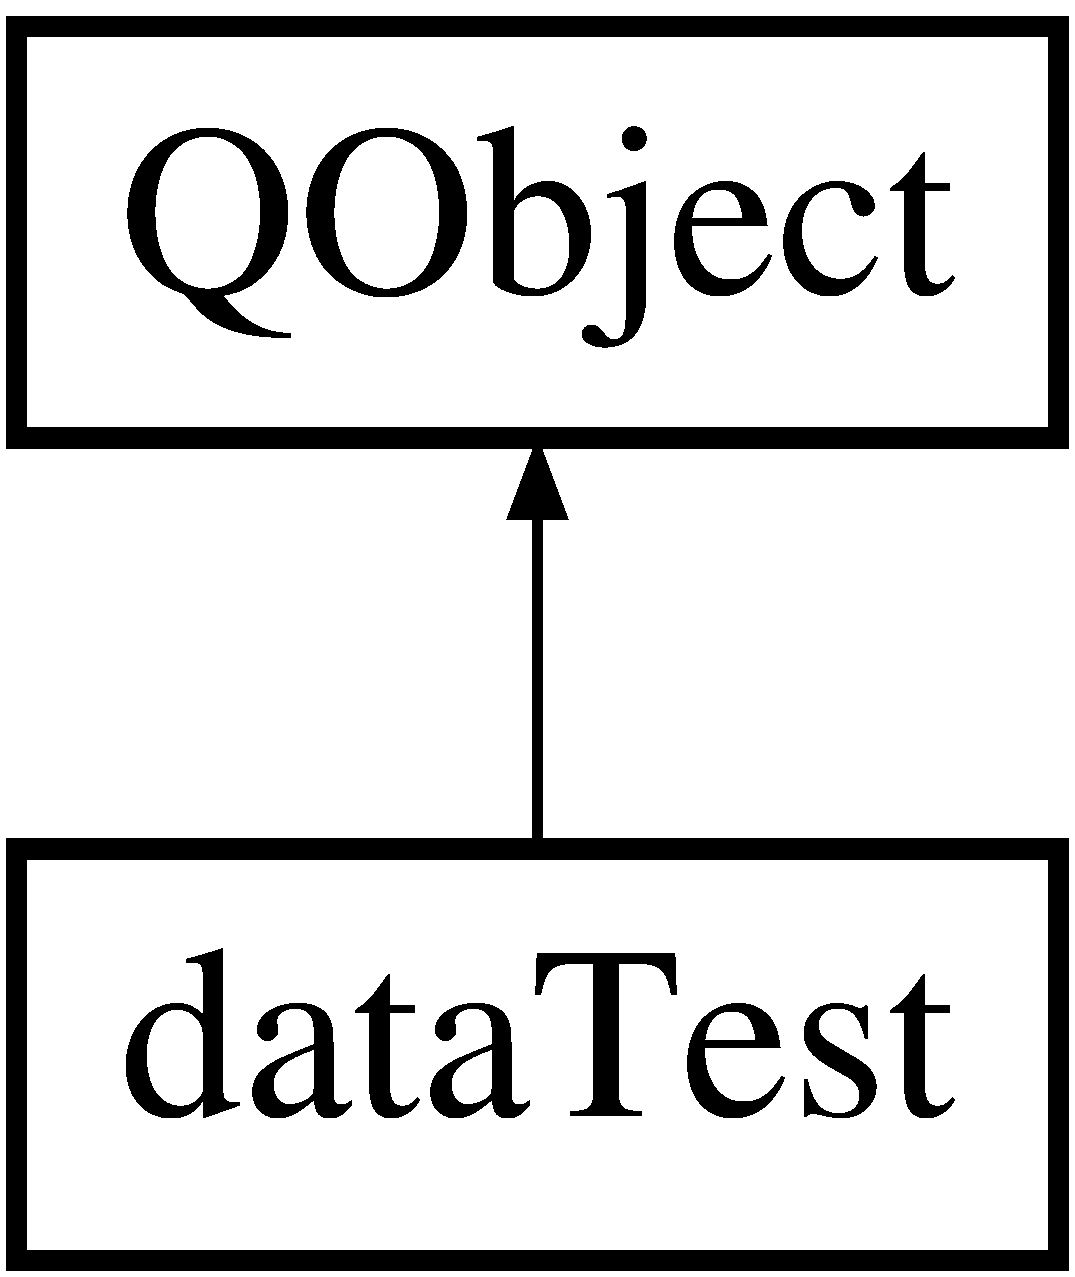
\includegraphics[height=2.000000cm]{classdata_test}
\end{center}
\end{figure}


\subsection{Подробное описание}


См. определение в файле tst\+\_\+data\+Test.\+cpp строка 4



Объявления и описания членов класса находятся в файле\+:\begin{DoxyCompactItemize}
\item 
kpk-\/data-\/test/\hyperlink{tst__data_test_8cpp}{tst\+\_\+data\+Test.\+cpp}\end{DoxyCompactItemize}

\hypertarget{classkpk_1_1core_1_1_db_service}{}\section{Класс kpk\+:\+:core\+:\+:Db\+Service}
\label{classkpk_1_1core_1_1_db_service}\index{kpk\+::core\+::\+Db\+Service@{kpk\+::core\+::\+Db\+Service}}


Служба управления базой данных  




{\ttfamily \#include $<$Db\+Service.\+h$>$}

\subsection*{Открытые члены}
\begin{DoxyCompactItemize}
\item 
\hyperlink{classkpk_1_1core_1_1_db_service_ad7213ea1a3e710889dcd06876c165d95}{Db\+Service} ()
\item 
\hyperlink{namespacekpk_1_1core_a466e66f45327171cc2976df1304573ab}{Db\+Ptr} \& \hyperlink{classkpk_1_1core_1_1_db_service_a185ef44041963592970695ecac61f3c3}{connect} ()
\begin{DoxyCompactList}\small\item\em Подключение к БД \end{DoxyCompactList}\item 
\hyperlink{namespacekpk_1_1core_a466e66f45327171cc2976df1304573ab}{Db\+Ptr} \& \hyperlink{classkpk_1_1core_1_1_db_service_a67de388a45320984577d9223918c13fb}{get} ()
\begin{DoxyCompactList}\small\item\em Получить объект БД \end{DoxyCompactList}\item 
\hyperlink{namespacekpk_1_1core_a466e66f45327171cc2976df1304573ab}{Db\+Ptr} \& \hyperlink{classkpk_1_1core_1_1_db_service_aacb6bafd43eda109a2888bb0d6f86892}{create\+Shcema} ()
\begin{DoxyCompactList}\small\item\em Создать схему \end{DoxyCompactList}\item 
void \hyperlink{classkpk_1_1core_1_1_db_service_a2fcdfaec8a98b2a6224bfbf7e6e0a3b9}{begin} ()
\begin{DoxyCompactList}\small\item\em Начало транзакции \end{DoxyCompactList}\item 
void \hyperlink{classkpk_1_1core_1_1_db_service_a819d4e51894ea9950d69d7d159003aa5}{commit} ()
\begin{DoxyCompactList}\small\item\em Фиксация транзакции \end{DoxyCompactList}\item 
void \hyperlink{classkpk_1_1core_1_1_db_service_a360724207bed795a2ca720961d2808a9}{rollback} ()
\begin{DoxyCompactList}\small\item\em Отмена транзакции \end{DoxyCompactList}\end{DoxyCompactItemize}


\subsection{Подробное описание}
Служба управления базой данных 

Подключение, создание, работа с транзакциями \begin{DoxyNote}{Заметки}
Строка\+:
\begin{DoxyCode}
odb::session \hyperlink{namespacekpk_1_1core_a4f9bed5f4644496878e2126c1c8e6412}{s}; 
\end{DoxyCode}
 в \hyperlink{_db_service_8cpp}{Db\+Service.\+cpp} нужна для возможности работать с двунаправленными отношениями (один-\/к-\/одному, один-\/ко-\/многим) (см. odb-\/manual п. 11 \char`\"{}\+Session\char`\"{}) 
\end{DoxyNote}


См. определение в файле Db\+Service.\+h строка 25



\subsection{Конструктор(ы)}
\index{kpk\+::core\+::\+Db\+Service@{kpk\+::core\+::\+Db\+Service}!Db\+Service@{Db\+Service}}
\index{Db\+Service@{Db\+Service}!kpk\+::core\+::\+Db\+Service@{kpk\+::core\+::\+Db\+Service}}
\subsubsection[{\texorpdfstring{Db\+Service()}{DbService()}}]{\setlength{\rightskip}{0pt plus 5cm}kpk\+::core\+::\+Db\+Service\+::\+Db\+Service (
\begin{DoxyParamCaption}
{}
\end{DoxyParamCaption}
)}\hypertarget{classkpk_1_1core_1_1_db_service_ad7213ea1a3e710889dcd06876c165d95}{}\label{classkpk_1_1core_1_1_db_service_ad7213ea1a3e710889dcd06876c165d95}


См. определение в файле Db\+Service.\+cpp строка 19



\subsection{Методы}
\index{kpk\+::core\+::\+Db\+Service@{kpk\+::core\+::\+Db\+Service}!begin@{begin}}
\index{begin@{begin}!kpk\+::core\+::\+Db\+Service@{kpk\+::core\+::\+Db\+Service}}
\subsubsection[{\texorpdfstring{begin()}{begin()}}]{\setlength{\rightskip}{0pt plus 5cm}void kpk\+::core\+::\+Db\+Service\+::begin (
\begin{DoxyParamCaption}
{}
\end{DoxyParamCaption}
)}\hypertarget{classkpk_1_1core_1_1_db_service_a2fcdfaec8a98b2a6224bfbf7e6e0a3b9}{}\label{classkpk_1_1core_1_1_db_service_a2fcdfaec8a98b2a6224bfbf7e6e0a3b9}


Начало транзакции 



См. определение в файле Db\+Service.\+cpp строка 86

\index{kpk\+::core\+::\+Db\+Service@{kpk\+::core\+::\+Db\+Service}!commit@{commit}}
\index{commit@{commit}!kpk\+::core\+::\+Db\+Service@{kpk\+::core\+::\+Db\+Service}}
\subsubsection[{\texorpdfstring{commit()}{commit()}}]{\setlength{\rightskip}{0pt plus 5cm}void kpk\+::core\+::\+Db\+Service\+::commit (
\begin{DoxyParamCaption}
{}
\end{DoxyParamCaption}
)}\hypertarget{classkpk_1_1core_1_1_db_service_a819d4e51894ea9950d69d7d159003aa5}{}\label{classkpk_1_1core_1_1_db_service_a819d4e51894ea9950d69d7d159003aa5}


Фиксация транзакции 



См. определение в файле Db\+Service.\+cpp строка 91

\index{kpk\+::core\+::\+Db\+Service@{kpk\+::core\+::\+Db\+Service}!connect@{connect}}
\index{connect@{connect}!kpk\+::core\+::\+Db\+Service@{kpk\+::core\+::\+Db\+Service}}
\subsubsection[{\texorpdfstring{connect()}{connect()}}]{\setlength{\rightskip}{0pt plus 5cm}{\bf Db\+Ptr} \& kpk\+::core\+::\+Db\+Service\+::connect (
\begin{DoxyParamCaption}
{}
\end{DoxyParamCaption}
)}\hypertarget{classkpk_1_1core_1_1_db_service_a185ef44041963592970695ecac61f3c3}{}\label{classkpk_1_1core_1_1_db_service_a185ef44041963592970695ecac61f3c3}


Подключение к БД 

\begin{DoxyReturn}{Возвращает}
Указатель на БД 
\end{DoxyReturn}


См. определение в файле Db\+Service.\+cpp строка 24

\index{kpk\+::core\+::\+Db\+Service@{kpk\+::core\+::\+Db\+Service}!create\+Shcema@{create\+Shcema}}
\index{create\+Shcema@{create\+Shcema}!kpk\+::core\+::\+Db\+Service@{kpk\+::core\+::\+Db\+Service}}
\subsubsection[{\texorpdfstring{create\+Shcema()}{createShcema()}}]{\setlength{\rightskip}{0pt plus 5cm}{\bf Db\+Ptr} \& kpk\+::core\+::\+Db\+Service\+::create\+Shcema (
\begin{DoxyParamCaption}
{}
\end{DoxyParamCaption}
)}\hypertarget{classkpk_1_1core_1_1_db_service_aacb6bafd43eda109a2888bb0d6f86892}{}\label{classkpk_1_1core_1_1_db_service_aacb6bafd43eda109a2888bb0d6f86892}


Создать схему 

\begin{DoxyReturn}{Возвращает}
Указатель на БД 
\end{DoxyReturn}


См. определение в файле Db\+Service.\+cpp строка 52

\index{kpk\+::core\+::\+Db\+Service@{kpk\+::core\+::\+Db\+Service}!get@{get}}
\index{get@{get}!kpk\+::core\+::\+Db\+Service@{kpk\+::core\+::\+Db\+Service}}
\subsubsection[{\texorpdfstring{get()}{get()}}]{\setlength{\rightskip}{0pt plus 5cm}{\bf Db\+Ptr} \& kpk\+::core\+::\+Db\+Service\+::get (
\begin{DoxyParamCaption}
{}
\end{DoxyParamCaption}
)}\hypertarget{classkpk_1_1core_1_1_db_service_a67de388a45320984577d9223918c13fb}{}\label{classkpk_1_1core_1_1_db_service_a67de388a45320984577d9223918c13fb}


Получить объект БД 

\begin{DoxyReturn}{Возвращает}
Указатель на БД 
\end{DoxyReturn}


См. определение в файле Db\+Service.\+cpp строка 47

\index{kpk\+::core\+::\+Db\+Service@{kpk\+::core\+::\+Db\+Service}!rollback@{rollback}}
\index{rollback@{rollback}!kpk\+::core\+::\+Db\+Service@{kpk\+::core\+::\+Db\+Service}}
\subsubsection[{\texorpdfstring{rollback()}{rollback()}}]{\setlength{\rightskip}{0pt plus 5cm}void kpk\+::core\+::\+Db\+Service\+::rollback (
\begin{DoxyParamCaption}
{}
\end{DoxyParamCaption}
)}\hypertarget{classkpk_1_1core_1_1_db_service_a360724207bed795a2ca720961d2808a9}{}\label{classkpk_1_1core_1_1_db_service_a360724207bed795a2ca720961d2808a9}


Отмена транзакции 



См. определение в файле Db\+Service.\+cpp строка 96



Объявления и описания членов классов находятся в файлах\+:\begin{DoxyCompactItemize}
\item 
kpk-\/core/\hyperlink{_db_service_8h}{Db\+Service.\+h}\item 
kpk-\/core/\hyperlink{_db_service_8cpp}{Db\+Service.\+cpp}\end{DoxyCompactItemize}

\hypertarget{classkpk_1_1test_1_1_kpk_core_test}{}\section{Класс kpk\+:\+:test\+:\+:Kpk\+Core\+Test}
\label{classkpk_1_1test_1_1_kpk_core_test}\index{kpk\+::test\+::\+Kpk\+Core\+Test@{kpk\+::test\+::\+Kpk\+Core\+Test}}
Граф наследования\+:kpk\+:\+:test\+:\+:Kpk\+Core\+Test\+:\begin{figure}[H]
\begin{center}
\leavevmode
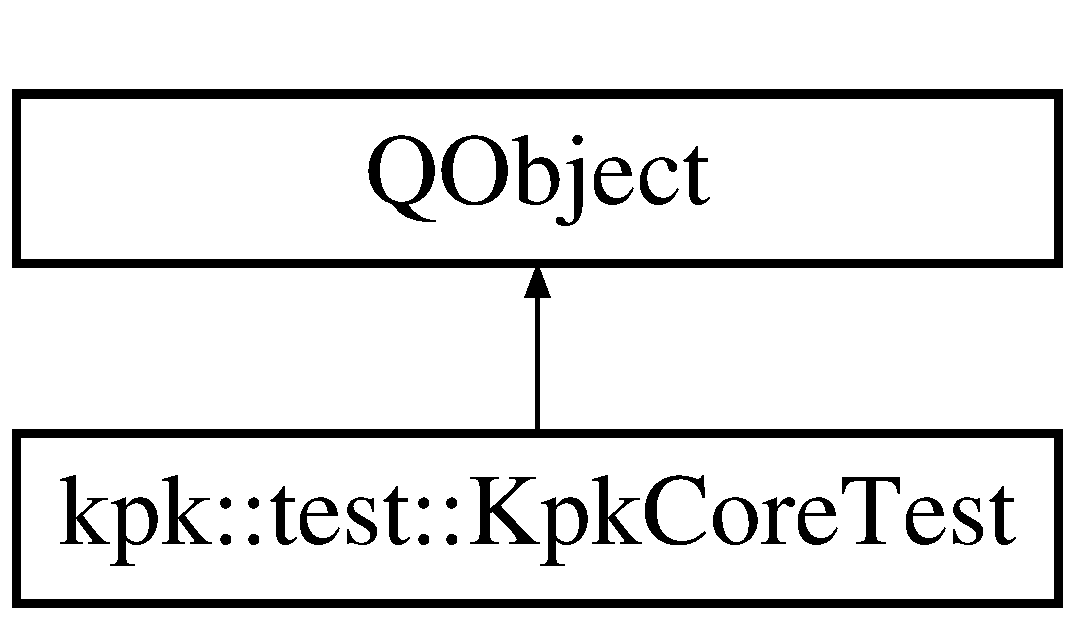
\includegraphics[height=2.000000cm]{classkpk_1_1test_1_1_kpk_core_test}
\end{center}
\end{figure}
\subsection*{Открытые члены}
\begin{DoxyCompactItemize}
\item 
\hyperlink{classkpk_1_1test_1_1_kpk_core_test_a39ca3c8af05c7b101cc23c4fd52ad2cd}{Kpk\+Core\+Test} ()
\end{DoxyCompactItemize}


\subsection{Подробное описание}


См. определение в файле tst\+\_\+\+Kpk\+Core\+Test.\+cpp строка 15



\subsection{Конструктор(ы)}
\index{kpk\+::test\+::\+Kpk\+Core\+Test@{kpk\+::test\+::\+Kpk\+Core\+Test}!Kpk\+Core\+Test@{Kpk\+Core\+Test}}
\index{Kpk\+Core\+Test@{Kpk\+Core\+Test}!kpk\+::test\+::\+Kpk\+Core\+Test@{kpk\+::test\+::\+Kpk\+Core\+Test}}
\subsubsection[{\texorpdfstring{Kpk\+Core\+Test()}{KpkCoreTest()}}]{\setlength{\rightskip}{0pt plus 5cm}kpk\+::test\+::\+Kpk\+Core\+Test\+::\+Kpk\+Core\+Test (
\begin{DoxyParamCaption}
{}
\end{DoxyParamCaption}
)}\hypertarget{classkpk_1_1test_1_1_kpk_core_test_a39ca3c8af05c7b101cc23c4fd52ad2cd}{}\label{classkpk_1_1test_1_1_kpk_core_test_a39ca3c8af05c7b101cc23c4fd52ad2cd}


См. определение в файле tst\+\_\+\+Kpk\+Core\+Test.\+cpp строка 33



Объявления и описания членов класса находятся в файле\+:\begin{DoxyCompactItemize}
\item 
kpk-\/core-\/test/\hyperlink{tst___kpk_core_test_8cpp}{tst\+\_\+\+Kpk\+Core\+Test.\+cpp}\end{DoxyCompactItemize}

\hypertarget{classkpk_1_1test_1_1kpk_data_test}{}\section{Класс kpk\+:\+:test\+:\+:kpk\+Data\+Test}
\label{classkpk_1_1test_1_1kpk_data_test}\index{kpk\+::test\+::kpk\+Data\+Test@{kpk\+::test\+::kpk\+Data\+Test}}
Граф наследования\+:kpk\+:\+:test\+:\+:kpk\+Data\+Test\+:\begin{figure}[H]
\begin{center}
\leavevmode
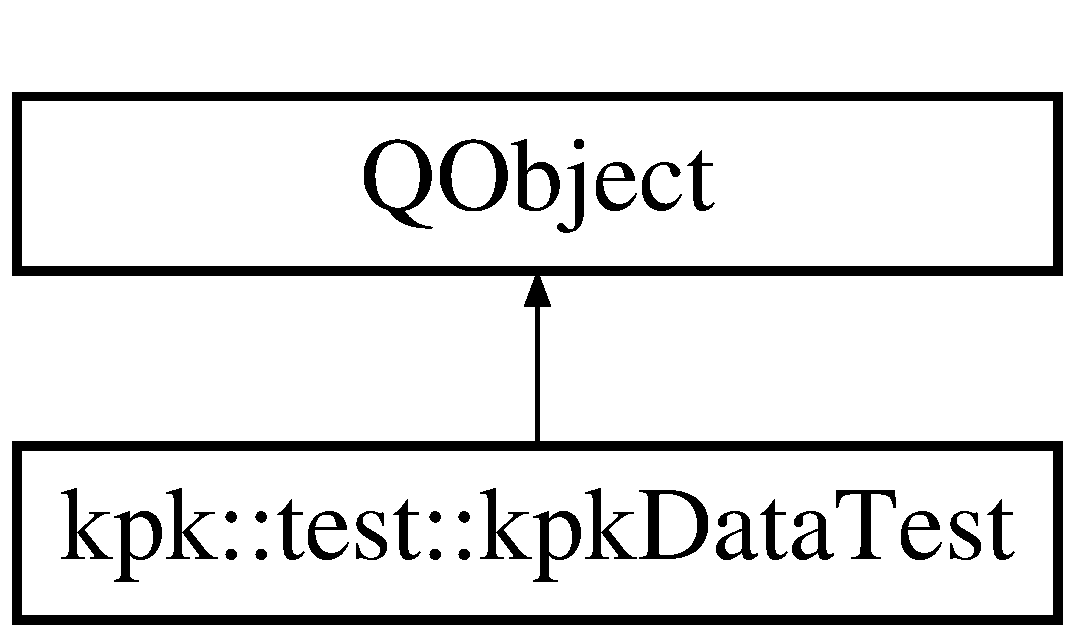
\includegraphics[height=2.000000cm]{classkpk_1_1test_1_1kpk_data_test}
\end{center}
\end{figure}
\subsection*{Открытые члены}
\begin{DoxyCompactItemize}
\item 
\hyperlink{classkpk_1_1test_1_1kpk_data_test_a15e675616bb8cffb23f3eace17bb4e76}{kpk\+Data\+Test} ()
\end{DoxyCompactItemize}


\subsection{Подробное описание}


См. определение в файле tst\+\_\+kpk\+Data\+Test.\+cpp строка 30



\subsection{Конструктор(ы)}
\index{kpk\+::test\+::kpk\+Data\+Test@{kpk\+::test\+::kpk\+Data\+Test}!kpk\+Data\+Test@{kpk\+Data\+Test}}
\index{kpk\+Data\+Test@{kpk\+Data\+Test}!kpk\+::test\+::kpk\+Data\+Test@{kpk\+::test\+::kpk\+Data\+Test}}
\subsubsection[{\texorpdfstring{kpk\+Data\+Test()}{kpkDataTest()}}]{\setlength{\rightskip}{0pt plus 5cm}kpk\+::test\+::kpk\+Data\+Test\+::kpk\+Data\+Test (
\begin{DoxyParamCaption}
{}
\end{DoxyParamCaption}
)}\hypertarget{classkpk_1_1test_1_1kpk_data_test_a15e675616bb8cffb23f3eace17bb4e76}{}\label{classkpk_1_1test_1_1kpk_data_test_a15e675616bb8cffb23f3eace17bb4e76}


См. определение в файле tst\+\_\+kpk\+Data\+Test.\+cpp строка 59



Объявления и описания членов класса находятся в файле\+:\begin{DoxyCompactItemize}
\item 
kpk-\/data-\/test/\hyperlink{tst__kpk_data_test_8cpp}{tst\+\_\+kpk\+Data\+Test.\+cpp}\end{DoxyCompactItemize}

\hypertarget{classkpk_1_1data_1_1_loan}{}\section{Класс kpk\+:\+:data\+:\+:Loan}
\label{classkpk_1_1data_1_1_loan}\index{kpk\+::data\+::\+Loan@{kpk\+::data\+::\+Loan}}


Займ  




{\ttfamily \#include $<$Loan.\+h$>$}

Граф наследования\+:kpk\+:\+:data\+:\+:Loan\+:\begin{figure}[H]
\begin{center}
\leavevmode
\includegraphics[height=2.000000cm]{classkpk_1_1data_1_1_loan}
\end{center}
\end{figure}
\subsection*{Открытые члены}
\begin{DoxyCompactItemize}
\item 
\hyperlink{classkpk_1_1data_1_1_loan_a466384959c1ccfaf4942c96c3409e6e6}{Loan} ()
\item 
\hyperlink{classkpk_1_1data_1_1_loan_afe8d8c50d04caef057413f2739599c82}{Loan} (std\+::shared\+\_\+ptr$<$ \hyperlink{classkpk_1_1data_1_1_member}{Member} $>$ \hyperlink{classkpk_1_1data_1_1_loan_a37fb3cc07280aa8310a32b4477b5528f}{member}, std\+::shared\+\_\+ptr$<$ \hyperlink{classkpk_1_1data_1_1_loan_type}{Loan\+Type} $>$ \hyperlink{classkpk_1_1data_1_1_loan_a791850364c82ef161f09669c64bcc2a3}{loan\+Type}, Q\+Date \hyperlink{classkpk_1_1data_1_1_loan_a0b039c0e6667da4f809f8e921f359f9b}{open\+Date}, Q\+Date \hyperlink{classkpk_1_1data_1_1_loan_af8ccbb954480eae0aa3b2a6b2f39fcb5}{close\+Date}, long \hyperlink{classkpk_1_1data_1_1_loan_ae82f80aa7a9b58fdfb2ac818dd33611d}{limit}, long \hyperlink{classkpk_1_1data_1_1_loan_affb2d1a39a5c7c185b07d5f6de87a43e}{rate}, long \hyperlink{classkpk_1_1data_1_1_loan_a89c1fd9e63d8923796f0cb3452bafa27}{length}, long \hyperlink{classkpk_1_1data_1_1_loan_a5b207380d82a2079ea83ec1ecf11f090}{sum}=0)
\begin{DoxyCompactList}\small\item\em Конструктор \end{DoxyCompactList}\item 
ulong \hyperlink{classkpk_1_1data_1_1_loan_a2827052c65d91b314bf1573ab56ffa3d}{id} ()
\begin{DoxyCompactList}\small\item\em Получить идентификатор \end{DoxyCompactList}\item 
Q\+Date \hyperlink{classkpk_1_1data_1_1_loan_a0b039c0e6667da4f809f8e921f359f9b}{open\+Date} ()
\begin{DoxyCompactList}\small\item\em Получить дату открытия \end{DoxyCompactList}\item 
void \hyperlink{classkpk_1_1data_1_1_loan_a46351e2f11a23a671e2a2d4be126eb2b}{open\+Date} (Q\+Date \&open\+Date)
\begin{DoxyCompactList}\small\item\em Установить дату открытия \end{DoxyCompactList}\item 
Q\+Date \hyperlink{classkpk_1_1data_1_1_loan_af8ccbb954480eae0aa3b2a6b2f39fcb5}{close\+Date} ()
\begin{DoxyCompactList}\small\item\em Получить дату завершения \end{DoxyCompactList}\item 
void \hyperlink{classkpk_1_1data_1_1_loan_ada266f079bcda1b9877ab161655c22e1}{close\+Date} (Q\+Date \&close\+Date)
\begin{DoxyCompactList}\small\item\em Установить дату завершения \end{DoxyCompactList}\item 
bool \hyperlink{classkpk_1_1data_1_1_loan_a70783859ac8c369fbacf45743b7dc527}{is\+Closed} () const 
\begin{DoxyCompactList}\small\item\em Закрыт ли займ \end{DoxyCompactList}\item 
void \hyperlink{classkpk_1_1data_1_1_loan_a582b7aa81d2087f14f69caf92254e865}{is\+Closed} (bool is\+Closed)
\begin{DoxyCompactList}\small\item\em Установить признак закрытия \end{DoxyCompactList}\item 
long \hyperlink{classkpk_1_1data_1_1_loan_affb2d1a39a5c7c185b07d5f6de87a43e}{rate} () const 
\begin{DoxyCompactList}\small\item\em Получить процентную ставку \end{DoxyCompactList}\item 
void \hyperlink{classkpk_1_1data_1_1_loan_aefef4f72d088471f5f32d1843c221108}{rate} (long rate)
\begin{DoxyCompactList}\small\item\em Установить процентную ставку \end{DoxyCompactList}\item 
long \hyperlink{classkpk_1_1data_1_1_loan_ae82f80aa7a9b58fdfb2ac818dd33611d}{limit} () const 
\begin{DoxyCompactList}\small\item\em Получить лимит кредитования \end{DoxyCompactList}\item 
void \hyperlink{classkpk_1_1data_1_1_loan_a83d5b22665f19627d26f3a57903511e6}{limit} (long limit)
\begin{DoxyCompactList}\small\item\em Установить лимит кредитования \end{DoxyCompactList}\item 
long \hyperlink{classkpk_1_1data_1_1_loan_a89c1fd9e63d8923796f0cb3452bafa27}{length} () const 
\begin{DoxyCompactList}\small\item\em Получить срок займа \end{DoxyCompactList}\item 
void \hyperlink{classkpk_1_1data_1_1_loan_af134c522e66faccb01b71c69c801ac6f}{length} (long length)
\begin{DoxyCompactList}\small\item\em Установить срок займа \end{DoxyCompactList}\item 
long \hyperlink{classkpk_1_1data_1_1_loan_a5b207380d82a2079ea83ec1ecf11f090}{sum} () const 
\begin{DoxyCompactList}\small\item\em Получить выданную сумма \end{DoxyCompactList}\item 
void \hyperlink{classkpk_1_1data_1_1_loan_a07ba28ed26a7a422b5c2435dbacd3825}{sum} (long sum)
\begin{DoxyCompactList}\small\item\em Установить выданную сумму \end{DoxyCompactList}\item 
long \hyperlink{classkpk_1_1data_1_1_loan_aabe63b94775011f6c971d8fb7a9cf5b0}{prc} () const 
\begin{DoxyCompactList}\small\item\em Получить начисленную компенсация \end{DoxyCompactList}\item 
void \hyperlink{classkpk_1_1data_1_1_loan_ae7141c53eac6c77d33c9e78eca17427d}{prc} (long prc)
\begin{DoxyCompactList}\small\item\em Установить начисленную компенсация \end{DoxyCompactList}\item 
long \hyperlink{classkpk_1_1data_1_1_loan_a3a85e20cceb9a563153d51fe07f15262}{remains} () const 
\begin{DoxyCompactList}\small\item\em Получить остаток займа \end{DoxyCompactList}\item 
void \hyperlink{classkpk_1_1data_1_1_loan_a242c59d916d1d2dd17d579bfac388e4a}{remains} (long remains)
\begin{DoxyCompactList}\small\item\em Установить остаток займа \end{DoxyCompactList}\item 
std\+::shared\+\_\+ptr$<$ \hyperlink{classkpk_1_1data_1_1_member}{Member} $>$ \hyperlink{classkpk_1_1data_1_1_loan_a37fb3cc07280aa8310a32b4477b5528f}{member} () const 
\begin{DoxyCompactList}\small\item\em Получить пайщика \end{DoxyCompactList}\item 
void \hyperlink{classkpk_1_1data_1_1_loan_afecd269c6ce5285602760df1bce52a41}{member} (const std\+::shared\+\_\+ptr$<$ \hyperlink{classkpk_1_1data_1_1_member}{Member} $>$ \&member)
\begin{DoxyCompactList}\small\item\em Установить пайщика \end{DoxyCompactList}\item 
std\+::shared\+\_\+ptr$<$ \hyperlink{classkpk_1_1data_1_1_person}{Person} $>$ \hyperlink{classkpk_1_1data_1_1_loan_abace5ace0d55d9e640a1d96fcd5c389b}{person} () const 
\begin{DoxyCompactList}\small\item\em Получить личные данные \end{DoxyCompactList}\item 
std\+::shared\+\_\+ptr$<$ \hyperlink{classkpk_1_1data_1_1_loan_type}{Loan\+Type} $>$ \hyperlink{classkpk_1_1data_1_1_loan_a791850364c82ef161f09669c64bcc2a3}{loan\+Type} () const 
\begin{DoxyCompactList}\small\item\em Получить вид займа \end{DoxyCompactList}\item 
void \hyperlink{classkpk_1_1data_1_1_loan_a4f6570e5a76b24dfa70009b0b60283a6}{loan\+Type} (const std\+::shared\+\_\+ptr$<$ \hyperlink{classkpk_1_1data_1_1_loan_type}{Loan\+Type} $>$ \&loan\+Type)
\begin{DoxyCompactList}\small\item\em Установить вид займа \end{DoxyCompactList}\end{DoxyCompactItemize}
\subsection*{Друзья}
\begin{DoxyCompactItemize}
\item 
class \hyperlink{classkpk_1_1data_1_1_loan_acb4d953abf85ae525f1d06a0c3a86a55}{odb\+::access}
\end{DoxyCompactItemize}
\subsection*{Дополнительные унаследованные члены}


\subsection{Подробное описание}
Займ 

См. определение в файле Loan.\+h строка 26



\subsection{Конструктор(ы)}
\index{kpk\+::data\+::\+Loan@{kpk\+::data\+::\+Loan}!Loan@{Loan}}
\index{Loan@{Loan}!kpk\+::data\+::\+Loan@{kpk\+::data\+::\+Loan}}
\subsubsection[{\texorpdfstring{Loan()}{Loan()}}]{\setlength{\rightskip}{0pt plus 5cm}kpk\+::data\+::\+Loan\+::\+Loan (
\begin{DoxyParamCaption}
{}
\end{DoxyParamCaption}
)}\hypertarget{classkpk_1_1data_1_1_loan_a466384959c1ccfaf4942c96c3409e6e6}{}\label{classkpk_1_1data_1_1_loan_a466384959c1ccfaf4942c96c3409e6e6}


См. определение в файле Loan.\+cpp строка 6

\index{kpk\+::data\+::\+Loan@{kpk\+::data\+::\+Loan}!Loan@{Loan}}
\index{Loan@{Loan}!kpk\+::data\+::\+Loan@{kpk\+::data\+::\+Loan}}
\subsubsection[{\texorpdfstring{Loan(std\+::shared\+\_\+ptr$<$ Member $>$ member, std\+::shared\+\_\+ptr$<$ Loan\+Type $>$ loan\+Type, Q\+Date open\+Date, Q\+Date close\+Date, long limit, long rate, long length, long sum=0)}{Loan(std::shared_ptr< Member > member, std::shared_ptr< LoanType > loanType, QDate openDate, QDate closeDate, long limit, long rate, long length, long sum=0)}}]{\setlength{\rightskip}{0pt plus 5cm}kpk\+::data\+::\+Loan\+::\+Loan (
\begin{DoxyParamCaption}
\item[{std\+::shared\+\_\+ptr$<$ {\bf Member} $>$}]{member, }
\item[{std\+::shared\+\_\+ptr$<$ {\bf Loan\+Type} $>$}]{loan\+Type, }
\item[{Q\+Date}]{open\+Date, }
\item[{Q\+Date}]{close\+Date, }
\item[{long}]{limit, }
\item[{long}]{rate, }
\item[{long}]{length, }
\item[{long}]{sum = {\ttfamily 0}}
\end{DoxyParamCaption}
)}\hypertarget{classkpk_1_1data_1_1_loan_afe8d8c50d04caef057413f2739599c82}{}\label{classkpk_1_1data_1_1_loan_afe8d8c50d04caef057413f2739599c82}


Конструктор 


\begin{DoxyParams}{Аргументы}
{\em member} & -\/ пайщик \\
\hline
{\em open\+Date} & -\/ дата открытия \\
\hline
{\em close\+Date} & -\/ дата завершения \\
\hline
{\em limit} & -\/ лимит кредитования \\
\hline
{\em rate} & -\/ ставка \\
\hline
{\em length} & -\/ срок \\
\hline
{\em sum} & -\/ выданная сумма \\
\hline
\end{DoxyParams}


См. определение в файле Loan.\+cpp строка 11



\subsection{Методы}
\index{kpk\+::data\+::\+Loan@{kpk\+::data\+::\+Loan}!close\+Date@{close\+Date}}
\index{close\+Date@{close\+Date}!kpk\+::data\+::\+Loan@{kpk\+::data\+::\+Loan}}
\subsubsection[{\texorpdfstring{close\+Date()}{closeDate()}}]{\setlength{\rightskip}{0pt plus 5cm}Q\+Date kpk\+::data\+::\+Loan\+::close\+Date (
\begin{DoxyParamCaption}
{}
\end{DoxyParamCaption}
)}\hypertarget{classkpk_1_1data_1_1_loan_af8ccbb954480eae0aa3b2a6b2f39fcb5}{}\label{classkpk_1_1data_1_1_loan_af8ccbb954480eae0aa3b2a6b2f39fcb5}


Получить дату завершения 

\begin{DoxyReturn}{Возвращает}
Дата завершения 
\end{DoxyReturn}


См. определение в файле Loan.\+cpp строка 43

\index{kpk\+::data\+::\+Loan@{kpk\+::data\+::\+Loan}!close\+Date@{close\+Date}}
\index{close\+Date@{close\+Date}!kpk\+::data\+::\+Loan@{kpk\+::data\+::\+Loan}}
\subsubsection[{\texorpdfstring{close\+Date(\+Q\+Date \&close\+Date)}{closeDate(QDate &closeDate)}}]{\setlength{\rightskip}{0pt plus 5cm}void kpk\+::data\+::\+Loan\+::close\+Date (
\begin{DoxyParamCaption}
\item[{Q\+Date \&}]{close\+Date}
\end{DoxyParamCaption}
)}\hypertarget{classkpk_1_1data_1_1_loan_ada266f079bcda1b9877ab161655c22e1}{}\label{classkpk_1_1data_1_1_loan_ada266f079bcda1b9877ab161655c22e1}


Установить дату завершения 


\begin{DoxyParams}{Аргументы}
{\em close\+Date} & -\/ дата завершения \\
\hline
\end{DoxyParams}


См. определение в файле Loan.\+cpp строка 48

\index{kpk\+::data\+::\+Loan@{kpk\+::data\+::\+Loan}!id@{id}}
\index{id@{id}!kpk\+::data\+::\+Loan@{kpk\+::data\+::\+Loan}}
\subsubsection[{\texorpdfstring{id()}{id()}}]{\setlength{\rightskip}{0pt plus 5cm}ulong kpk\+::data\+::\+Loan\+::id (
\begin{DoxyParamCaption}
{}
\end{DoxyParamCaption}
)}\hypertarget{classkpk_1_1data_1_1_loan_a2827052c65d91b314bf1573ab56ffa3d}{}\label{classkpk_1_1data_1_1_loan_a2827052c65d91b314bf1573ab56ffa3d}


Получить идентификатор 

\begin{DoxyReturn}{Возвращает}
Идентификатор 
\end{DoxyReturn}


См. определение в файле Loan.\+cpp строка 28

\index{kpk\+::data\+::\+Loan@{kpk\+::data\+::\+Loan}!is\+Closed@{is\+Closed}}
\index{is\+Closed@{is\+Closed}!kpk\+::data\+::\+Loan@{kpk\+::data\+::\+Loan}}
\subsubsection[{\texorpdfstring{is\+Closed() const }{isClosed() const }}]{\setlength{\rightskip}{0pt plus 5cm}bool kpk\+::data\+::\+Loan\+::is\+Closed (
\begin{DoxyParamCaption}
{}
\end{DoxyParamCaption}
) const}\hypertarget{classkpk_1_1data_1_1_loan_a70783859ac8c369fbacf45743b7dc527}{}\label{classkpk_1_1data_1_1_loan_a70783859ac8c369fbacf45743b7dc527}


Закрыт ли займ 

\begin{DoxyReturn}{Возвращает}
Признак закрытия 
\end{DoxyReturn}


См. определение в файле Loan.\+cpp строка 79

\index{kpk\+::data\+::\+Loan@{kpk\+::data\+::\+Loan}!is\+Closed@{is\+Closed}}
\index{is\+Closed@{is\+Closed}!kpk\+::data\+::\+Loan@{kpk\+::data\+::\+Loan}}
\subsubsection[{\texorpdfstring{is\+Closed(bool is\+Closed)}{isClosed(bool isClosed)}}]{\setlength{\rightskip}{0pt plus 5cm}void kpk\+::data\+::\+Loan\+::is\+Closed (
\begin{DoxyParamCaption}
\item[{bool}]{is\+Closed}
\end{DoxyParamCaption}
)}\hypertarget{classkpk_1_1data_1_1_loan_a582b7aa81d2087f14f69caf92254e865}{}\label{classkpk_1_1data_1_1_loan_a582b7aa81d2087f14f69caf92254e865}


Установить признак закрытия 


\begin{DoxyParams}{Аргументы}
{\em is\+Closed} & -\/ признак закрытия \\
\hline
\end{DoxyParams}


См. определение в файле Loan.\+cpp строка 84

\index{kpk\+::data\+::\+Loan@{kpk\+::data\+::\+Loan}!length@{length}}
\index{length@{length}!kpk\+::data\+::\+Loan@{kpk\+::data\+::\+Loan}}
\subsubsection[{\texorpdfstring{length() const }{length() const }}]{\setlength{\rightskip}{0pt plus 5cm}long kpk\+::data\+::\+Loan\+::length (
\begin{DoxyParamCaption}
{}
\end{DoxyParamCaption}
) const}\hypertarget{classkpk_1_1data_1_1_loan_a89c1fd9e63d8923796f0cb3452bafa27}{}\label{classkpk_1_1data_1_1_loan_a89c1fd9e63d8923796f0cb3452bafa27}


Получить срок займа 

\begin{DoxyReturn}{Возвращает}
Срок займа 
\end{DoxyReturn}


См. определение в файле Loan.\+cpp строка 109

\index{kpk\+::data\+::\+Loan@{kpk\+::data\+::\+Loan}!length@{length}}
\index{length@{length}!kpk\+::data\+::\+Loan@{kpk\+::data\+::\+Loan}}
\subsubsection[{\texorpdfstring{length(long length)}{length(long length)}}]{\setlength{\rightskip}{0pt plus 5cm}void kpk\+::data\+::\+Loan\+::length (
\begin{DoxyParamCaption}
\item[{long}]{length}
\end{DoxyParamCaption}
)}\hypertarget{classkpk_1_1data_1_1_loan_af134c522e66faccb01b71c69c801ac6f}{}\label{classkpk_1_1data_1_1_loan_af134c522e66faccb01b71c69c801ac6f}


Установить срок займа 


\begin{DoxyParams}{Аргументы}
{\em length} & -\/ срок займа \\
\hline
\end{DoxyParams}


См. определение в файле Loan.\+cpp строка 114

\index{kpk\+::data\+::\+Loan@{kpk\+::data\+::\+Loan}!limit@{limit}}
\index{limit@{limit}!kpk\+::data\+::\+Loan@{kpk\+::data\+::\+Loan}}
\subsubsection[{\texorpdfstring{limit() const }{limit() const }}]{\setlength{\rightskip}{0pt plus 5cm}long kpk\+::data\+::\+Loan\+::limit (
\begin{DoxyParamCaption}
{}
\end{DoxyParamCaption}
) const}\hypertarget{classkpk_1_1data_1_1_loan_ae82f80aa7a9b58fdfb2ac818dd33611d}{}\label{classkpk_1_1data_1_1_loan_ae82f80aa7a9b58fdfb2ac818dd33611d}


Получить лимит кредитования 

Максимальная сумма займа \begin{DoxyReturn}{Возвращает}
Лимит кредитования 
\end{DoxyReturn}


См. определение в файле Loan.\+cpp строка 99

\index{kpk\+::data\+::\+Loan@{kpk\+::data\+::\+Loan}!limit@{limit}}
\index{limit@{limit}!kpk\+::data\+::\+Loan@{kpk\+::data\+::\+Loan}}
\subsubsection[{\texorpdfstring{limit(long limit)}{limit(long limit)}}]{\setlength{\rightskip}{0pt plus 5cm}void kpk\+::data\+::\+Loan\+::limit (
\begin{DoxyParamCaption}
\item[{long}]{limit}
\end{DoxyParamCaption}
)}\hypertarget{classkpk_1_1data_1_1_loan_a83d5b22665f19627d26f3a57903511e6}{}\label{classkpk_1_1data_1_1_loan_a83d5b22665f19627d26f3a57903511e6}


Установить лимит кредитования 

Максимальная сумма займа 
\begin{DoxyParams}{Аргументы}
{\em limit} & -\/ Лимит кредитования \\
\hline
\end{DoxyParams}


См. определение в файле Loan.\+cpp строка 104

\index{kpk\+::data\+::\+Loan@{kpk\+::data\+::\+Loan}!loan\+Type@{loan\+Type}}
\index{loan\+Type@{loan\+Type}!kpk\+::data\+::\+Loan@{kpk\+::data\+::\+Loan}}
\subsubsection[{\texorpdfstring{loan\+Type() const }{loanType() const }}]{\setlength{\rightskip}{0pt plus 5cm}std\+::shared\+\_\+ptr$<$ {\bf Loan\+Type} $>$ kpk\+::data\+::\+Loan\+::loan\+Type (
\begin{DoxyParamCaption}
{}
\end{DoxyParamCaption}
) const}\hypertarget{classkpk_1_1data_1_1_loan_a791850364c82ef161f09669c64bcc2a3}{}\label{classkpk_1_1data_1_1_loan_a791850364c82ef161f09669c64bcc2a3}


Получить вид займа 

\begin{DoxyReturn}{Возвращает}
Вид займа 
\end{DoxyReturn}


См. определение в файле Loan.\+cpp строка 69

\index{kpk\+::data\+::\+Loan@{kpk\+::data\+::\+Loan}!loan\+Type@{loan\+Type}}
\index{loan\+Type@{loan\+Type}!kpk\+::data\+::\+Loan@{kpk\+::data\+::\+Loan}}
\subsubsection[{\texorpdfstring{loan\+Type(const std\+::shared\+\_\+ptr$<$ Loan\+Type $>$ \&loan\+Type)}{loanType(const std::shared_ptr< LoanType > &loanType)}}]{\setlength{\rightskip}{0pt plus 5cm}void kpk\+::data\+::\+Loan\+::loan\+Type (
\begin{DoxyParamCaption}
\item[{const std\+::shared\+\_\+ptr$<$ {\bf Loan\+Type} $>$ \&}]{loan\+Type}
\end{DoxyParamCaption}
)}\hypertarget{classkpk_1_1data_1_1_loan_a4f6570e5a76b24dfa70009b0b60283a6}{}\label{classkpk_1_1data_1_1_loan_a4f6570e5a76b24dfa70009b0b60283a6}


Установить вид займа 


\begin{DoxyParams}{Аргументы}
{\em loan\+Type} & -\/ вид займа \\
\hline
\end{DoxyParams}


См. определение в файле Loan.\+cpp строка 74

\index{kpk\+::data\+::\+Loan@{kpk\+::data\+::\+Loan}!member@{member}}
\index{member@{member}!kpk\+::data\+::\+Loan@{kpk\+::data\+::\+Loan}}
\subsubsection[{\texorpdfstring{member() const }{member() const }}]{\setlength{\rightskip}{0pt plus 5cm}std\+::shared\+\_\+ptr$<$ {\bf Member} $>$ kpk\+::data\+::\+Loan\+::member (
\begin{DoxyParamCaption}
{}
\end{DoxyParamCaption}
) const}\hypertarget{classkpk_1_1data_1_1_loan_a37fb3cc07280aa8310a32b4477b5528f}{}\label{classkpk_1_1data_1_1_loan_a37fb3cc07280aa8310a32b4477b5528f}


Получить пайщика 

\begin{DoxyReturn}{Возвращает}
Пайщик 
\end{DoxyReturn}


См. определение в файле Loan.\+cpp строка 53

\index{kpk\+::data\+::\+Loan@{kpk\+::data\+::\+Loan}!member@{member}}
\index{member@{member}!kpk\+::data\+::\+Loan@{kpk\+::data\+::\+Loan}}
\subsubsection[{\texorpdfstring{member(const std\+::shared\+\_\+ptr$<$ Member $>$ \&member)}{member(const std::shared_ptr< Member > &member)}}]{\setlength{\rightskip}{0pt plus 5cm}void kpk\+::data\+::\+Loan\+::member (
\begin{DoxyParamCaption}
\item[{const std\+::shared\+\_\+ptr$<$ {\bf Member} $>$ \&}]{member}
\end{DoxyParamCaption}
)}\hypertarget{classkpk_1_1data_1_1_loan_afecd269c6ce5285602760df1bce52a41}{}\label{classkpk_1_1data_1_1_loan_afecd269c6ce5285602760df1bce52a41}


Установить пайщика 


\begin{DoxyParams}{Аргументы}
{\em member} & -\/ пайщик \\
\hline
\end{DoxyParams}


См. определение в файле Loan.\+cpp строка 58

\index{kpk\+::data\+::\+Loan@{kpk\+::data\+::\+Loan}!open\+Date@{open\+Date}}
\index{open\+Date@{open\+Date}!kpk\+::data\+::\+Loan@{kpk\+::data\+::\+Loan}}
\subsubsection[{\texorpdfstring{open\+Date()}{openDate()}}]{\setlength{\rightskip}{0pt plus 5cm}Q\+Date kpk\+::data\+::\+Loan\+::open\+Date (
\begin{DoxyParamCaption}
{}
\end{DoxyParamCaption}
)}\hypertarget{classkpk_1_1data_1_1_loan_a0b039c0e6667da4f809f8e921f359f9b}{}\label{classkpk_1_1data_1_1_loan_a0b039c0e6667da4f809f8e921f359f9b}


Получить дату открытия 

\begin{DoxyReturn}{Возвращает}
Дата открытия 
\end{DoxyReturn}


См. определение в файле Loan.\+cpp строка 33

\index{kpk\+::data\+::\+Loan@{kpk\+::data\+::\+Loan}!open\+Date@{open\+Date}}
\index{open\+Date@{open\+Date}!kpk\+::data\+::\+Loan@{kpk\+::data\+::\+Loan}}
\subsubsection[{\texorpdfstring{open\+Date(\+Q\+Date \&open\+Date)}{openDate(QDate &openDate)}}]{\setlength{\rightskip}{0pt plus 5cm}void kpk\+::data\+::\+Loan\+::open\+Date (
\begin{DoxyParamCaption}
\item[{Q\+Date \&}]{open\+Date}
\end{DoxyParamCaption}
)}\hypertarget{classkpk_1_1data_1_1_loan_a46351e2f11a23a671e2a2d4be126eb2b}{}\label{classkpk_1_1data_1_1_loan_a46351e2f11a23a671e2a2d4be126eb2b}


Установить дату открытия 


\begin{DoxyParams}{Аргументы}
{\em open\+Date} & -\/ дата открытия \\
\hline
\end{DoxyParams}


См. определение в файле Loan.\+cpp строка 38

\index{kpk\+::data\+::\+Loan@{kpk\+::data\+::\+Loan}!person@{person}}
\index{person@{person}!kpk\+::data\+::\+Loan@{kpk\+::data\+::\+Loan}}
\subsubsection[{\texorpdfstring{person() const }{person() const }}]{\setlength{\rightskip}{0pt plus 5cm}std\+::shared\+\_\+ptr$<$ {\bf Person} $>$ kpk\+::data\+::\+Loan\+::person (
\begin{DoxyParamCaption}
{}
\end{DoxyParamCaption}
) const}\hypertarget{classkpk_1_1data_1_1_loan_abace5ace0d55d9e640a1d96fcd5c389b}{}\label{classkpk_1_1data_1_1_loan_abace5ace0d55d9e640a1d96fcd5c389b}


Получить личные данные 

\begin{DoxyReturn}{Возвращает}
личные данные 
\end{DoxyReturn}


См. определение в файле Loan.\+cpp строка 64

\index{kpk\+::data\+::\+Loan@{kpk\+::data\+::\+Loan}!prc@{prc}}
\index{prc@{prc}!kpk\+::data\+::\+Loan@{kpk\+::data\+::\+Loan}}
\subsubsection[{\texorpdfstring{prc() const }{prc() const }}]{\setlength{\rightskip}{0pt plus 5cm}long kpk\+::data\+::\+Loan\+::prc (
\begin{DoxyParamCaption}
{}
\end{DoxyParamCaption}
) const}\hypertarget{classkpk_1_1data_1_1_loan_aabe63b94775011f6c971d8fb7a9cf5b0}{}\label{classkpk_1_1data_1_1_loan_aabe63b94775011f6c971d8fb7a9cf5b0}


Получить начисленную компенсация 

\begin{DoxyReturn}{Возвращает}
Начисленная компенсация 
\end{DoxyReturn}


См. определение в файле Loan.\+cpp строка 129

\index{kpk\+::data\+::\+Loan@{kpk\+::data\+::\+Loan}!prc@{prc}}
\index{prc@{prc}!kpk\+::data\+::\+Loan@{kpk\+::data\+::\+Loan}}
\subsubsection[{\texorpdfstring{prc(long prc)}{prc(long prc)}}]{\setlength{\rightskip}{0pt plus 5cm}void kpk\+::data\+::\+Loan\+::prc (
\begin{DoxyParamCaption}
\item[{long}]{prc}
\end{DoxyParamCaption}
)}\hypertarget{classkpk_1_1data_1_1_loan_ae7141c53eac6c77d33c9e78eca17427d}{}\label{classkpk_1_1data_1_1_loan_ae7141c53eac6c77d33c9e78eca17427d}


Установить начисленную компенсация 


\begin{DoxyParams}{Аргументы}
{\em prc} & -\/ начисленная компенсация \\
\hline
\end{DoxyParams}


См. определение в файле Loan.\+cpp строка 134

\index{kpk\+::data\+::\+Loan@{kpk\+::data\+::\+Loan}!rate@{rate}}
\index{rate@{rate}!kpk\+::data\+::\+Loan@{kpk\+::data\+::\+Loan}}
\subsubsection[{\texorpdfstring{rate() const }{rate() const }}]{\setlength{\rightskip}{0pt plus 5cm}long kpk\+::data\+::\+Loan\+::rate (
\begin{DoxyParamCaption}
{}
\end{DoxyParamCaption}
) const}\hypertarget{classkpk_1_1data_1_1_loan_affb2d1a39a5c7c185b07d5f6de87a43e}{}\label{classkpk_1_1data_1_1_loan_affb2d1a39a5c7c185b07d5f6de87a43e}


Получить процентную ставку 

\begin{DoxyReturn}{Возвращает}
Процентная ставка 
\end{DoxyReturn}


См. определение в файле Loan.\+cpp строка 89

\index{kpk\+::data\+::\+Loan@{kpk\+::data\+::\+Loan}!rate@{rate}}
\index{rate@{rate}!kpk\+::data\+::\+Loan@{kpk\+::data\+::\+Loan}}
\subsubsection[{\texorpdfstring{rate(long rate)}{rate(long rate)}}]{\setlength{\rightskip}{0pt plus 5cm}void kpk\+::data\+::\+Loan\+::rate (
\begin{DoxyParamCaption}
\item[{long}]{rate}
\end{DoxyParamCaption}
)}\hypertarget{classkpk_1_1data_1_1_loan_aefef4f72d088471f5f32d1843c221108}{}\label{classkpk_1_1data_1_1_loan_aefef4f72d088471f5f32d1843c221108}


Установить процентную ставку 


\begin{DoxyParams}{Аргументы}
{\em rate} & -\/ процентная ставка \\
\hline
\end{DoxyParams}


См. определение в файле Loan.\+cpp строка 94

\index{kpk\+::data\+::\+Loan@{kpk\+::data\+::\+Loan}!remains@{remains}}
\index{remains@{remains}!kpk\+::data\+::\+Loan@{kpk\+::data\+::\+Loan}}
\subsubsection[{\texorpdfstring{remains() const }{remains() const }}]{\setlength{\rightskip}{0pt plus 5cm}long kpk\+::data\+::\+Loan\+::remains (
\begin{DoxyParamCaption}
{}
\end{DoxyParamCaption}
) const}\hypertarget{classkpk_1_1data_1_1_loan_a3a85e20cceb9a563153d51fe07f15262}{}\label{classkpk_1_1data_1_1_loan_a3a85e20cceb9a563153d51fe07f15262}


Получить остаток займа 

\begin{DoxyReturn}{Возвращает}
остаток займа 
\end{DoxyReturn}


См. определение в файле Loan.\+cpp строка 139

\index{kpk\+::data\+::\+Loan@{kpk\+::data\+::\+Loan}!remains@{remains}}
\index{remains@{remains}!kpk\+::data\+::\+Loan@{kpk\+::data\+::\+Loan}}
\subsubsection[{\texorpdfstring{remains(long remains)}{remains(long remains)}}]{\setlength{\rightskip}{0pt plus 5cm}void kpk\+::data\+::\+Loan\+::remains (
\begin{DoxyParamCaption}
\item[{long}]{remains}
\end{DoxyParamCaption}
)}\hypertarget{classkpk_1_1data_1_1_loan_a242c59d916d1d2dd17d579bfac388e4a}{}\label{classkpk_1_1data_1_1_loan_a242c59d916d1d2dd17d579bfac388e4a}


Установить остаток займа 


\begin{DoxyParams}{Аргументы}
{\em remains} & -\/ остаток займа \\
\hline
\end{DoxyParams}


См. определение в файле Loan.\+cpp строка 144

\index{kpk\+::data\+::\+Loan@{kpk\+::data\+::\+Loan}!sum@{sum}}
\index{sum@{sum}!kpk\+::data\+::\+Loan@{kpk\+::data\+::\+Loan}}
\subsubsection[{\texorpdfstring{sum() const }{sum() const }}]{\setlength{\rightskip}{0pt plus 5cm}long kpk\+::data\+::\+Loan\+::sum (
\begin{DoxyParamCaption}
{}
\end{DoxyParamCaption}
) const}\hypertarget{classkpk_1_1data_1_1_loan_a5b207380d82a2079ea83ec1ecf11f090}{}\label{classkpk_1_1data_1_1_loan_a5b207380d82a2079ea83ec1ecf11f090}


Получить выданную сумма 

\begin{DoxyReturn}{Возвращает}
Выданная сумма 
\end{DoxyReturn}


См. определение в файле Loan.\+cpp строка 119

\index{kpk\+::data\+::\+Loan@{kpk\+::data\+::\+Loan}!sum@{sum}}
\index{sum@{sum}!kpk\+::data\+::\+Loan@{kpk\+::data\+::\+Loan}}
\subsubsection[{\texorpdfstring{sum(long sum)}{sum(long sum)}}]{\setlength{\rightskip}{0pt plus 5cm}void kpk\+::data\+::\+Loan\+::sum (
\begin{DoxyParamCaption}
\item[{long}]{sum}
\end{DoxyParamCaption}
)}\hypertarget{classkpk_1_1data_1_1_loan_a07ba28ed26a7a422b5c2435dbacd3825}{}\label{classkpk_1_1data_1_1_loan_a07ba28ed26a7a422b5c2435dbacd3825}


Установить выданную сумму 


\begin{DoxyParams}{Аргументы}
{\em sum} & -\/ выданная сумма \\
\hline
\end{DoxyParams}


См. определение в файле Loan.\+cpp строка 124



\subsection{Документация по друзьям класса и функциям, относящимся к классу}
\index{kpk\+::data\+::\+Loan@{kpk\+::data\+::\+Loan}!odb\+::access@{odb\+::access}}
\index{odb\+::access@{odb\+::access}!kpk\+::data\+::\+Loan@{kpk\+::data\+::\+Loan}}
\subsubsection[{\texorpdfstring{odb\+::access}{odb::access}}]{\setlength{\rightskip}{0pt plus 5cm}friend class odb\+::access\hspace{0.3cm}{\ttfamily [friend]}}\hypertarget{classkpk_1_1data_1_1_loan_acb4d953abf85ae525f1d06a0c3a86a55}{}\label{classkpk_1_1data_1_1_loan_acb4d953abf85ae525f1d06a0c3a86a55}


См. определение в файле Loan.\+h строка 193



Объявления и описания членов классов находятся в файлах\+:\begin{DoxyCompactItemize}
\item 
kpk-\/data/\hyperlink{_loan_8h}{Loan.\+h}\item 
kpk-\/data/\hyperlink{_loan_8cpp}{Loan.\+cpp}\end{DoxyCompactItemize}

\hypertarget{classkpk_1_1data_1_1_loan_oper}{}\section{Класс kpk\+:\+:data\+:\+:Loan\+Oper}
\label{classkpk_1_1data_1_1_loan_oper}\index{kpk\+::data\+::\+Loan\+Oper@{kpk\+::data\+::\+Loan\+Oper}}


Операция по займу  




{\ttfamily \#include $<$Loan\+Oper.\+h$>$}

\subsection*{Открытые члены}
\begin{DoxyCompactItemize}
\item 
\hyperlink{classkpk_1_1data_1_1_loan_oper_ab4c52cd423192f6d8a14bac56917e8cb}{Loan\+Oper} ()
\item 
\hyperlink{classkpk_1_1data_1_1_loan_oper_value}{Loan\+Oper\+Value} \& \hyperlink{classkpk_1_1data_1_1_loan_oper_af20e426695913f8593131a65014b29b4}{plan} ()
\begin{DoxyCompactList}\small\item\em Получить оплату по плану \end{DoxyCompactList}\item 
\hyperlink{classkpk_1_1data_1_1_loan_oper_value}{Loan\+Oper\+Value} \& \hyperlink{classkpk_1_1data_1_1_loan_oper_afab5ad2be6f0207bce3c61e2b6ea8f40}{fact} ()
\begin{DoxyCompactList}\small\item\em Получить оплату по факту \end{DoxyCompactList}\item 
std\+::shared\+\_\+ptr$<$ \hyperlink{classkpk_1_1data_1_1_member}{Member} $>$ \hyperlink{classkpk_1_1data_1_1_loan_oper_a18b2bace5fa76d8fe05e275edd88b604}{member} () const 
\begin{DoxyCompactList}\small\item\em Получить пайщика \end{DoxyCompactList}\item 
void \hyperlink{classkpk_1_1data_1_1_loan_oper_af5ac012ec26a5380d0df9ed2f263c8cd}{member} (const std\+::shared\+\_\+ptr$<$ \hyperlink{classkpk_1_1data_1_1_member}{Member} $>$ \&member)
\begin{DoxyCompactList}\small\item\em Установить пайщика \end{DoxyCompactList}\item 
std\+::shared\+\_\+ptr$<$ \hyperlink{classkpk_1_1data_1_1_person}{Person} $>$ \hyperlink{classkpk_1_1data_1_1_loan_oper_a20f5a2088eb043664cc127bcf2f1fe37}{person} () const 
\begin{DoxyCompactList}\small\item\em Получить личные данные \end{DoxyCompactList}\item 
std\+::shared\+\_\+ptr$<$ \hyperlink{classkpk_1_1data_1_1_loan}{Loan} $>$ \hyperlink{classkpk_1_1data_1_1_loan_oper_a112db60dae0b1e3f2e40c8c3a2444848}{loan} () const 
\begin{DoxyCompactList}\small\item\em Получить займ \end{DoxyCompactList}\item 
void \hyperlink{classkpk_1_1data_1_1_loan_oper_af46beb664e0021f8939e70de3c89ab50}{loan} (const std\+::shared\+\_\+ptr$<$ \hyperlink{classkpk_1_1data_1_1_loan}{Loan} $>$ \&loan)
\begin{DoxyCompactList}\small\item\em Установить займ \end{DoxyCompactList}\end{DoxyCompactItemize}
\subsection*{Друзья}
\begin{DoxyCompactItemize}
\item 
class \hyperlink{classkpk_1_1data_1_1_loan_oper_acb4d953abf85ae525f1d06a0c3a86a55}{odb\+::access}
\end{DoxyCompactItemize}


\subsection{Подробное описание}
Операция по займу 

Операция по займу (оплата или выдача) 

См. определение в файле Loan\+Oper.\+h строка 25



\subsection{Конструктор(ы)}
\index{kpk\+::data\+::\+Loan\+Oper@{kpk\+::data\+::\+Loan\+Oper}!Loan\+Oper@{Loan\+Oper}}
\index{Loan\+Oper@{Loan\+Oper}!kpk\+::data\+::\+Loan\+Oper@{kpk\+::data\+::\+Loan\+Oper}}
\subsubsection[{\texorpdfstring{Loan\+Oper()}{LoanOper()}}]{\setlength{\rightskip}{0pt plus 5cm}kpk\+::data\+::\+Loan\+Oper\+::\+Loan\+Oper (
\begin{DoxyParamCaption}
{}
\end{DoxyParamCaption}
)}\hypertarget{classkpk_1_1data_1_1_loan_oper_ab4c52cd423192f6d8a14bac56917e8cb}{}\label{classkpk_1_1data_1_1_loan_oper_ab4c52cd423192f6d8a14bac56917e8cb}


См. определение в файле Loan\+Oper.\+cpp строка 7



\subsection{Методы}
\index{kpk\+::data\+::\+Loan\+Oper@{kpk\+::data\+::\+Loan\+Oper}!fact@{fact}}
\index{fact@{fact}!kpk\+::data\+::\+Loan\+Oper@{kpk\+::data\+::\+Loan\+Oper}}
\subsubsection[{\texorpdfstring{fact()}{fact()}}]{\setlength{\rightskip}{0pt plus 5cm}{\bf Loan\+Oper\+Value} \& kpk\+::data\+::\+Loan\+Oper\+::fact (
\begin{DoxyParamCaption}
{}
\end{DoxyParamCaption}
)}\hypertarget{classkpk_1_1data_1_1_loan_oper_afab5ad2be6f0207bce3c61e2b6ea8f40}{}\label{classkpk_1_1data_1_1_loan_oper_afab5ad2be6f0207bce3c61e2b6ea8f40}


Получить оплату по факту 

\begin{DoxyReturn}{Возвращает}
Оплата по факту 
\end{DoxyReturn}


См. определение в файле Loan\+Oper.\+cpp строка 17

\index{kpk\+::data\+::\+Loan\+Oper@{kpk\+::data\+::\+Loan\+Oper}!loan@{loan}}
\index{loan@{loan}!kpk\+::data\+::\+Loan\+Oper@{kpk\+::data\+::\+Loan\+Oper}}
\subsubsection[{\texorpdfstring{loan() const }{loan() const }}]{\setlength{\rightskip}{0pt plus 5cm}std\+::shared\+\_\+ptr$<$ {\bf Loan} $>$ kpk\+::data\+::\+Loan\+Oper\+::loan (
\begin{DoxyParamCaption}
{}
\end{DoxyParamCaption}
) const}\hypertarget{classkpk_1_1data_1_1_loan_oper_a112db60dae0b1e3f2e40c8c3a2444848}{}\label{classkpk_1_1data_1_1_loan_oper_a112db60dae0b1e3f2e40c8c3a2444848}


Получить займ 

\begin{DoxyReturn}{Возвращает}
Займ 
\end{DoxyReturn}


См. определение в файле Loan\+Oper.\+cpp строка 39

\index{kpk\+::data\+::\+Loan\+Oper@{kpk\+::data\+::\+Loan\+Oper}!loan@{loan}}
\index{loan@{loan}!kpk\+::data\+::\+Loan\+Oper@{kpk\+::data\+::\+Loan\+Oper}}
\subsubsection[{\texorpdfstring{loan(const std\+::shared\+\_\+ptr$<$ Loan $>$ \&loan)}{loan(const std::shared_ptr< Loan > &loan)}}]{\setlength{\rightskip}{0pt plus 5cm}void kpk\+::data\+::\+Loan\+Oper\+::loan (
\begin{DoxyParamCaption}
\item[{const std\+::shared\+\_\+ptr$<$ {\bf Loan} $>$ \&}]{loan}
\end{DoxyParamCaption}
)}\hypertarget{classkpk_1_1data_1_1_loan_oper_af46beb664e0021f8939e70de3c89ab50}{}\label{classkpk_1_1data_1_1_loan_oper_af46beb664e0021f8939e70de3c89ab50}


Установить займ 


\begin{DoxyParams}{Аргументы}
{\em loan} & -\/ займ \\
\hline
\end{DoxyParams}


См. определение в файле Loan\+Oper.\+cpp строка 44

\index{kpk\+::data\+::\+Loan\+Oper@{kpk\+::data\+::\+Loan\+Oper}!member@{member}}
\index{member@{member}!kpk\+::data\+::\+Loan\+Oper@{kpk\+::data\+::\+Loan\+Oper}}
\subsubsection[{\texorpdfstring{member() const }{member() const }}]{\setlength{\rightskip}{0pt plus 5cm}std\+::shared\+\_\+ptr$<$ {\bf Member} $>$ kpk\+::data\+::\+Loan\+Oper\+::member (
\begin{DoxyParamCaption}
{}
\end{DoxyParamCaption}
) const}\hypertarget{classkpk_1_1data_1_1_loan_oper_a18b2bace5fa76d8fe05e275edd88b604}{}\label{classkpk_1_1data_1_1_loan_oper_a18b2bace5fa76d8fe05e275edd88b604}


Получить пайщика 

\begin{DoxyReturn}{Возвращает}
Пайщик 
\end{DoxyReturn}


См. определение в файле Loan\+Oper.\+cpp строка 23

\index{kpk\+::data\+::\+Loan\+Oper@{kpk\+::data\+::\+Loan\+Oper}!member@{member}}
\index{member@{member}!kpk\+::data\+::\+Loan\+Oper@{kpk\+::data\+::\+Loan\+Oper}}
\subsubsection[{\texorpdfstring{member(const std\+::shared\+\_\+ptr$<$ Member $>$ \&member)}{member(const std::shared_ptr< Member > &member)}}]{\setlength{\rightskip}{0pt plus 5cm}void kpk\+::data\+::\+Loan\+Oper\+::member (
\begin{DoxyParamCaption}
\item[{const std\+::shared\+\_\+ptr$<$ {\bf Member} $>$ \&}]{member}
\end{DoxyParamCaption}
)}\hypertarget{classkpk_1_1data_1_1_loan_oper_af5ac012ec26a5380d0df9ed2f263c8cd}{}\label{classkpk_1_1data_1_1_loan_oper_af5ac012ec26a5380d0df9ed2f263c8cd}


Установить пайщика 


\begin{DoxyParams}{Аргументы}
{\em member} & -\/ пайщик \\
\hline
\end{DoxyParams}


См. определение в файле Loan\+Oper.\+cpp строка 28

\index{kpk\+::data\+::\+Loan\+Oper@{kpk\+::data\+::\+Loan\+Oper}!person@{person}}
\index{person@{person}!kpk\+::data\+::\+Loan\+Oper@{kpk\+::data\+::\+Loan\+Oper}}
\subsubsection[{\texorpdfstring{person() const }{person() const }}]{\setlength{\rightskip}{0pt plus 5cm}std\+::shared\+\_\+ptr$<$ {\bf Person} $>$ kpk\+::data\+::\+Loan\+Oper\+::person (
\begin{DoxyParamCaption}
{}
\end{DoxyParamCaption}
) const}\hypertarget{classkpk_1_1data_1_1_loan_oper_a20f5a2088eb043664cc127bcf2f1fe37}{}\label{classkpk_1_1data_1_1_loan_oper_a20f5a2088eb043664cc127bcf2f1fe37}


Получить личные данные 

\begin{DoxyReturn}{Возвращает}
Личные данные 
\end{DoxyReturn}


См. определение в файле Loan\+Oper.\+cpp строка 34

\index{kpk\+::data\+::\+Loan\+Oper@{kpk\+::data\+::\+Loan\+Oper}!plan@{plan}}
\index{plan@{plan}!kpk\+::data\+::\+Loan\+Oper@{kpk\+::data\+::\+Loan\+Oper}}
\subsubsection[{\texorpdfstring{plan()}{plan()}}]{\setlength{\rightskip}{0pt plus 5cm}{\bf Loan\+Oper\+Value} \& kpk\+::data\+::\+Loan\+Oper\+::plan (
\begin{DoxyParamCaption}
{}
\end{DoxyParamCaption}
)}\hypertarget{classkpk_1_1data_1_1_loan_oper_af20e426695913f8593131a65014b29b4}{}\label{classkpk_1_1data_1_1_loan_oper_af20e426695913f8593131a65014b29b4}


Получить оплату по плану 

\begin{DoxyReturn}{Возвращает}
Оплата по плану 
\end{DoxyReturn}


См. определение в файле Loan\+Oper.\+cpp строка 12



\subsection{Документация по друзьям класса и функциям, относящимся к классу}
\index{kpk\+::data\+::\+Loan\+Oper@{kpk\+::data\+::\+Loan\+Oper}!odb\+::access@{odb\+::access}}
\index{odb\+::access@{odb\+::access}!kpk\+::data\+::\+Loan\+Oper@{kpk\+::data\+::\+Loan\+Oper}}
\subsubsection[{\texorpdfstring{odb\+::access}{odb::access}}]{\setlength{\rightskip}{0pt plus 5cm}friend class odb\+::access\hspace{0.3cm}{\ttfamily [friend]}}\hypertarget{classkpk_1_1data_1_1_loan_oper_acb4d953abf85ae525f1d06a0c3a86a55}{}\label{classkpk_1_1data_1_1_loan_oper_acb4d953abf85ae525f1d06a0c3a86a55}


См. определение в файле Loan\+Oper.\+h строка 73



Объявления и описания членов классов находятся в файлах\+:\begin{DoxyCompactItemize}
\item 
kpk-\/data/\hyperlink{_loan_oper_8h}{Loan\+Oper.\+h}\item 
kpk-\/data/\hyperlink{_loan_oper_8cpp}{Loan\+Oper.\+cpp}\end{DoxyCompactItemize}

\hypertarget{classkpk_1_1data_1_1_loan_oper_value}{}\section{Класс kpk\+:\+:data\+:\+:Loan\+Oper\+Value}
\label{classkpk_1_1data_1_1_loan_oper_value}\index{kpk\+::data\+::\+Loan\+Oper\+Value@{kpk\+::data\+::\+Loan\+Oper\+Value}}


Данные операции по займу  




{\ttfamily \#include $<$Loan\+Oper\+Value.\+h$>$}

\subsection*{Открытые члены}
\begin{DoxyCompactItemize}
\item 
\hyperlink{classkpk_1_1data_1_1_loan_oper_value_a85a3528d4888aa7977098f2641b2cf12}{Loan\+Oper\+Value} ()
\item 
Q\+Date \hyperlink{classkpk_1_1data_1_1_loan_oper_value_a79a69dfe8b0585d044da833ae6fb499c}{date} () const 
\begin{DoxyCompactList}\small\item\em Получить дату \end{DoxyCompactList}\item 
void \hyperlink{classkpk_1_1data_1_1_loan_oper_value_a666ebe276be1ee68f7daa6b71b32102e}{date} (const Q\+Date \&date)
\begin{DoxyCompactList}\small\item\em Установить дату \end{DoxyCompactList}\item 
long \hyperlink{classkpk_1_1data_1_1_loan_oper_value_a7c02ccfb03583b86685063c794bfb127}{amount} () const 
\begin{DoxyCompactList}\small\item\em Получить плную сумму оплаты \end{DoxyCompactList}\item 
void \hyperlink{classkpk_1_1data_1_1_loan_oper_value_a674d9125b2b2529a05c83aa3247488ea}{amount} (long amount)
\begin{DoxyCompactList}\small\item\em Установить полную сумму оплаты \end{DoxyCompactList}\item 
long \hyperlink{classkpk_1_1data_1_1_loan_oper_value_a62abaf1afa796f4ab870b3eaf28c52a3}{loan} () const 
\begin{DoxyCompactList}\small\item\em Получить основной долг \end{DoxyCompactList}\item 
void \hyperlink{classkpk_1_1data_1_1_loan_oper_value_ab5e5d0809777c84ba37e4799e5049441}{loan} (long loan)
\begin{DoxyCompactList}\small\item\em Установить основной долг \end{DoxyCompactList}\item 
long \hyperlink{classkpk_1_1data_1_1_loan_oper_value_a7bf3672ba4a76178c9ac56c9bfb7d41c}{loan\+Dept} () const 
\begin{DoxyCompactList}\small\item\em Получить задолженность по осноному долгу \end{DoxyCompactList}\item 
void \hyperlink{classkpk_1_1data_1_1_loan_oper_value_a3018a5c77b71f5cbf7b770a63d619c8b}{loan\+Dept} (long loan\+Dept)
\begin{DoxyCompactList}\small\item\em Установить задолженность по осноному долгу \end{DoxyCompactList}\item 
long \hyperlink{classkpk_1_1data_1_1_loan_oper_value_a73063afb20f403339b47a1459b5cf0e8}{prc} () const 
\begin{DoxyCompactList}\small\item\em Получить компенсацию \end{DoxyCompactList}\item 
void \hyperlink{classkpk_1_1data_1_1_loan_oper_value_aeb8f5417e33bedd2ad4fa5af05265be6}{prc} (long prc)
\begin{DoxyCompactList}\small\item\em Установить компенсацию \end{DoxyCompactList}\item 
long \hyperlink{classkpk_1_1data_1_1_loan_oper_value_a4ec5046e4e88a88d1fe753c8f4767f79}{prc\+Dept} () const 
\begin{DoxyCompactList}\small\item\em Получить задолженностиь по компенсации \end{DoxyCompactList}\item 
void \hyperlink{classkpk_1_1data_1_1_loan_oper_value_a4c054186ad90a49951ae2a4ee9d29331}{prc\+Dept} (long prc\+Dept)
\begin{DoxyCompactList}\small\item\em Установить задолженность по компенсации \end{DoxyCompactList}\item 
long \hyperlink{classkpk_1_1data_1_1_loan_oper_value_a10b14d39ece49ca7ce6cc3b71ae3413d}{peni} () const 
\begin{DoxyCompactList}\small\item\em Получить неустойку \end{DoxyCompactList}\item 
void \hyperlink{classkpk_1_1data_1_1_loan_oper_value_af3834e6064f5dfd1fa5544e0f54adb4a}{peni} (long peni)
\begin{DoxyCompactList}\small\item\em Установить неустойку \end{DoxyCompactList}\end{DoxyCompactItemize}
\subsection*{Друзья}
\begin{DoxyCompactItemize}
\item 
class \hyperlink{classkpk_1_1data_1_1_loan_oper_value_acb4d953abf85ae525f1d06a0c3a86a55}{odb\+::access}
\end{DoxyCompactItemize}


\subsection{Подробное описание}
Данные операции по займу 

См. определение в файле Loan\+Oper\+Value.\+h строка 16



\subsection{Конструктор(ы)}
\index{kpk\+::data\+::\+Loan\+Oper\+Value@{kpk\+::data\+::\+Loan\+Oper\+Value}!Loan\+Oper\+Value@{Loan\+Oper\+Value}}
\index{Loan\+Oper\+Value@{Loan\+Oper\+Value}!kpk\+::data\+::\+Loan\+Oper\+Value@{kpk\+::data\+::\+Loan\+Oper\+Value}}
\subsubsection[{\texorpdfstring{Loan\+Oper\+Value()}{LoanOperValue()}}]{\setlength{\rightskip}{0pt plus 5cm}kpk\+::data\+::\+Loan\+Oper\+Value\+::\+Loan\+Oper\+Value (
\begin{DoxyParamCaption}
{}
\end{DoxyParamCaption}
)}\hypertarget{classkpk_1_1data_1_1_loan_oper_value_a85a3528d4888aa7977098f2641b2cf12}{}\label{classkpk_1_1data_1_1_loan_oper_value_a85a3528d4888aa7977098f2641b2cf12}


См. определение в файле Loan\+Oper\+Value.\+cpp строка 7



\subsection{Методы}
\index{kpk\+::data\+::\+Loan\+Oper\+Value@{kpk\+::data\+::\+Loan\+Oper\+Value}!amount@{amount}}
\index{amount@{amount}!kpk\+::data\+::\+Loan\+Oper\+Value@{kpk\+::data\+::\+Loan\+Oper\+Value}}
\subsubsection[{\texorpdfstring{amount() const }{amount() const }}]{\setlength{\rightskip}{0pt plus 5cm}long kpk\+::data\+::\+Loan\+Oper\+Value\+::amount (
\begin{DoxyParamCaption}
{}
\end{DoxyParamCaption}
) const}\hypertarget{classkpk_1_1data_1_1_loan_oper_value_a7c02ccfb03583b86685063c794bfb127}{}\label{classkpk_1_1data_1_1_loan_oper_value_a7c02ccfb03583b86685063c794bfb127}


Получить плную сумму оплаты 

\begin{DoxyReturn}{Возвращает}
Полная сумма оплаты 
\end{DoxyReturn}


См. определение в файле Loan\+Oper\+Value.\+cpp строка 22

\index{kpk\+::data\+::\+Loan\+Oper\+Value@{kpk\+::data\+::\+Loan\+Oper\+Value}!amount@{amount}}
\index{amount@{amount}!kpk\+::data\+::\+Loan\+Oper\+Value@{kpk\+::data\+::\+Loan\+Oper\+Value}}
\subsubsection[{\texorpdfstring{amount(long amount)}{amount(long amount)}}]{\setlength{\rightskip}{0pt plus 5cm}void kpk\+::data\+::\+Loan\+Oper\+Value\+::amount (
\begin{DoxyParamCaption}
\item[{long}]{amount}
\end{DoxyParamCaption}
)}\hypertarget{classkpk_1_1data_1_1_loan_oper_value_a674d9125b2b2529a05c83aa3247488ea}{}\label{classkpk_1_1data_1_1_loan_oper_value_a674d9125b2b2529a05c83aa3247488ea}


Установить полную сумму оплаты 


\begin{DoxyParams}{Аргументы}
{\em amount} & -\/ полная сумма оплаты \\
\hline
\end{DoxyParams}


См. определение в файле Loan\+Oper\+Value.\+cpp строка 27

\index{kpk\+::data\+::\+Loan\+Oper\+Value@{kpk\+::data\+::\+Loan\+Oper\+Value}!date@{date}}
\index{date@{date}!kpk\+::data\+::\+Loan\+Oper\+Value@{kpk\+::data\+::\+Loan\+Oper\+Value}}
\subsubsection[{\texorpdfstring{date() const }{date() const }}]{\setlength{\rightskip}{0pt plus 5cm}Q\+Date kpk\+::data\+::\+Loan\+Oper\+Value\+::date (
\begin{DoxyParamCaption}
{}
\end{DoxyParamCaption}
) const}\hypertarget{classkpk_1_1data_1_1_loan_oper_value_a79a69dfe8b0585d044da833ae6fb499c}{}\label{classkpk_1_1data_1_1_loan_oper_value_a79a69dfe8b0585d044da833ae6fb499c}


Получить дату 

\begin{DoxyReturn}{Возвращает}
дата 
\end{DoxyReturn}


См. определение в файле Loan\+Oper\+Value.\+cpp строка 12

\index{kpk\+::data\+::\+Loan\+Oper\+Value@{kpk\+::data\+::\+Loan\+Oper\+Value}!date@{date}}
\index{date@{date}!kpk\+::data\+::\+Loan\+Oper\+Value@{kpk\+::data\+::\+Loan\+Oper\+Value}}
\subsubsection[{\texorpdfstring{date(const Q\+Date \&date)}{date(const QDate &date)}}]{\setlength{\rightskip}{0pt plus 5cm}void kpk\+::data\+::\+Loan\+Oper\+Value\+::date (
\begin{DoxyParamCaption}
\item[{const Q\+Date \&}]{date}
\end{DoxyParamCaption}
)}\hypertarget{classkpk_1_1data_1_1_loan_oper_value_a666ebe276be1ee68f7daa6b71b32102e}{}\label{classkpk_1_1data_1_1_loan_oper_value_a666ebe276be1ee68f7daa6b71b32102e}


Установить дату 


\begin{DoxyParams}{Аргументы}
{\em дата} & \\
\hline
\end{DoxyParams}


См. определение в файле Loan\+Oper\+Value.\+cpp строка 17

\index{kpk\+::data\+::\+Loan\+Oper\+Value@{kpk\+::data\+::\+Loan\+Oper\+Value}!loan@{loan}}
\index{loan@{loan}!kpk\+::data\+::\+Loan\+Oper\+Value@{kpk\+::data\+::\+Loan\+Oper\+Value}}
\subsubsection[{\texorpdfstring{loan() const }{loan() const }}]{\setlength{\rightskip}{0pt plus 5cm}long kpk\+::data\+::\+Loan\+Oper\+Value\+::loan (
\begin{DoxyParamCaption}
{}
\end{DoxyParamCaption}
) const}\hypertarget{classkpk_1_1data_1_1_loan_oper_value_a62abaf1afa796f4ab870b3eaf28c52a3}{}\label{classkpk_1_1data_1_1_loan_oper_value_a62abaf1afa796f4ab870b3eaf28c52a3}


Получить основной долг 

Получить сумму оплаты основного долга \begin{DoxyReturn}{Возвращает}
Сумма оплаты основного долга 
\end{DoxyReturn}


См. определение в файле Loan\+Oper\+Value.\+cpp строка 32

\index{kpk\+::data\+::\+Loan\+Oper\+Value@{kpk\+::data\+::\+Loan\+Oper\+Value}!loan@{loan}}
\index{loan@{loan}!kpk\+::data\+::\+Loan\+Oper\+Value@{kpk\+::data\+::\+Loan\+Oper\+Value}}
\subsubsection[{\texorpdfstring{loan(long loan)}{loan(long loan)}}]{\setlength{\rightskip}{0pt plus 5cm}void kpk\+::data\+::\+Loan\+Oper\+Value\+::loan (
\begin{DoxyParamCaption}
\item[{long}]{loan}
\end{DoxyParamCaption}
)}\hypertarget{classkpk_1_1data_1_1_loan_oper_value_ab5e5d0809777c84ba37e4799e5049441}{}\label{classkpk_1_1data_1_1_loan_oper_value_ab5e5d0809777c84ba37e4799e5049441}


Установить основной долг 

Установить сумму оплаты основного долга 
\begin{DoxyParams}{Аргументы}
{\em loan} & -\/ cумма оплаты основного долга \\
\hline
\end{DoxyParams}


См. определение в файле Loan\+Oper\+Value.\+cpp строка 37

\index{kpk\+::data\+::\+Loan\+Oper\+Value@{kpk\+::data\+::\+Loan\+Oper\+Value}!loan\+Dept@{loan\+Dept}}
\index{loan\+Dept@{loan\+Dept}!kpk\+::data\+::\+Loan\+Oper\+Value@{kpk\+::data\+::\+Loan\+Oper\+Value}}
\subsubsection[{\texorpdfstring{loan\+Dept() const }{loanDept() const }}]{\setlength{\rightskip}{0pt plus 5cm}long kpk\+::data\+::\+Loan\+Oper\+Value\+::loan\+Dept (
\begin{DoxyParamCaption}
{}
\end{DoxyParamCaption}
) const}\hypertarget{classkpk_1_1data_1_1_loan_oper_value_a7bf3672ba4a76178c9ac56c9bfb7d41c}{}\label{classkpk_1_1data_1_1_loan_oper_value_a7bf3672ba4a76178c9ac56c9bfb7d41c}


Получить задолженность по осноному долгу 

Получить сумму оплаты задолженности по осноному долгу \begin{DoxyReturn}{Возвращает}
Задолженность по осноному долгу 
\end{DoxyReturn}


См. определение в файле Loan\+Oper\+Value.\+cpp строка 42

\index{kpk\+::data\+::\+Loan\+Oper\+Value@{kpk\+::data\+::\+Loan\+Oper\+Value}!loan\+Dept@{loan\+Dept}}
\index{loan\+Dept@{loan\+Dept}!kpk\+::data\+::\+Loan\+Oper\+Value@{kpk\+::data\+::\+Loan\+Oper\+Value}}
\subsubsection[{\texorpdfstring{loan\+Dept(long loan\+Dept)}{loanDept(long loanDept)}}]{\setlength{\rightskip}{0pt plus 5cm}void kpk\+::data\+::\+Loan\+Oper\+Value\+::loan\+Dept (
\begin{DoxyParamCaption}
\item[{long}]{loan\+Dept}
\end{DoxyParamCaption}
)}\hypertarget{classkpk_1_1data_1_1_loan_oper_value_a3018a5c77b71f5cbf7b770a63d619c8b}{}\label{classkpk_1_1data_1_1_loan_oper_value_a3018a5c77b71f5cbf7b770a63d619c8b}


Установить задолженность по осноному долгу 

Установить сумму оплаты задолженности по осноному долгу 
\begin{DoxyParams}{Аргументы}
{\em loan\+Dept} & -\/ задолженность по осноному долгу \\
\hline
\end{DoxyParams}


См. определение в файле Loan\+Oper\+Value.\+cpp строка 47

\index{kpk\+::data\+::\+Loan\+Oper\+Value@{kpk\+::data\+::\+Loan\+Oper\+Value}!peni@{peni}}
\index{peni@{peni}!kpk\+::data\+::\+Loan\+Oper\+Value@{kpk\+::data\+::\+Loan\+Oper\+Value}}
\subsubsection[{\texorpdfstring{peni() const }{peni() const }}]{\setlength{\rightskip}{0pt plus 5cm}long kpk\+::data\+::\+Loan\+Oper\+Value\+::peni (
\begin{DoxyParamCaption}
{}
\end{DoxyParamCaption}
) const}\hypertarget{classkpk_1_1data_1_1_loan_oper_value_a10b14d39ece49ca7ce6cc3b71ae3413d}{}\label{classkpk_1_1data_1_1_loan_oper_value_a10b14d39ece49ca7ce6cc3b71ae3413d}


Получить неустойку 

\begin{DoxyReturn}{Возвращает}
неустойка 
\end{DoxyReturn}


См. определение в файле Loan\+Oper\+Value.\+cpp строка 72

\index{kpk\+::data\+::\+Loan\+Oper\+Value@{kpk\+::data\+::\+Loan\+Oper\+Value}!peni@{peni}}
\index{peni@{peni}!kpk\+::data\+::\+Loan\+Oper\+Value@{kpk\+::data\+::\+Loan\+Oper\+Value}}
\subsubsection[{\texorpdfstring{peni(long peni)}{peni(long peni)}}]{\setlength{\rightskip}{0pt plus 5cm}void kpk\+::data\+::\+Loan\+Oper\+Value\+::peni (
\begin{DoxyParamCaption}
\item[{long}]{peni}
\end{DoxyParamCaption}
)}\hypertarget{classkpk_1_1data_1_1_loan_oper_value_af3834e6064f5dfd1fa5544e0f54adb4a}{}\label{classkpk_1_1data_1_1_loan_oper_value_af3834e6064f5dfd1fa5544e0f54adb4a}


Установить неустойку 


\begin{DoxyParams}{Аргументы}
{\em peni} & -\/ неустойка \\
\hline
\end{DoxyParams}


См. определение в файле Loan\+Oper\+Value.\+cpp строка 77

\index{kpk\+::data\+::\+Loan\+Oper\+Value@{kpk\+::data\+::\+Loan\+Oper\+Value}!prc@{prc}}
\index{prc@{prc}!kpk\+::data\+::\+Loan\+Oper\+Value@{kpk\+::data\+::\+Loan\+Oper\+Value}}
\subsubsection[{\texorpdfstring{prc() const }{prc() const }}]{\setlength{\rightskip}{0pt plus 5cm}long kpk\+::data\+::\+Loan\+Oper\+Value\+::prc (
\begin{DoxyParamCaption}
{}
\end{DoxyParamCaption}
) const}\hypertarget{classkpk_1_1data_1_1_loan_oper_value_a73063afb20f403339b47a1459b5cf0e8}{}\label{classkpk_1_1data_1_1_loan_oper_value_a73063afb20f403339b47a1459b5cf0e8}


Получить компенсацию 

Получить сумму оплаты компенсации \begin{DoxyReturn}{Возвращает}
Сумма оплаты компенсации 
\end{DoxyReturn}


См. определение в файле Loan\+Oper\+Value.\+cpp строка 52

\index{kpk\+::data\+::\+Loan\+Oper\+Value@{kpk\+::data\+::\+Loan\+Oper\+Value}!prc@{prc}}
\index{prc@{prc}!kpk\+::data\+::\+Loan\+Oper\+Value@{kpk\+::data\+::\+Loan\+Oper\+Value}}
\subsubsection[{\texorpdfstring{prc(long prc)}{prc(long prc)}}]{\setlength{\rightskip}{0pt plus 5cm}void kpk\+::data\+::\+Loan\+Oper\+Value\+::prc (
\begin{DoxyParamCaption}
\item[{long}]{prc}
\end{DoxyParamCaption}
)}\hypertarget{classkpk_1_1data_1_1_loan_oper_value_aeb8f5417e33bedd2ad4fa5af05265be6}{}\label{classkpk_1_1data_1_1_loan_oper_value_aeb8f5417e33bedd2ad4fa5af05265be6}


Установить компенсацию 

Установить сумму оплаты компенсации 
\begin{DoxyParams}{Аргументы}
{\em prc} & -\/ сумма оплаты компенсации \\
\hline
\end{DoxyParams}


См. определение в файле Loan\+Oper\+Value.\+cpp строка 57

\index{kpk\+::data\+::\+Loan\+Oper\+Value@{kpk\+::data\+::\+Loan\+Oper\+Value}!prc\+Dept@{prc\+Dept}}
\index{prc\+Dept@{prc\+Dept}!kpk\+::data\+::\+Loan\+Oper\+Value@{kpk\+::data\+::\+Loan\+Oper\+Value}}
\subsubsection[{\texorpdfstring{prc\+Dept() const }{prcDept() const }}]{\setlength{\rightskip}{0pt plus 5cm}long kpk\+::data\+::\+Loan\+Oper\+Value\+::prc\+Dept (
\begin{DoxyParamCaption}
{}
\end{DoxyParamCaption}
) const}\hypertarget{classkpk_1_1data_1_1_loan_oper_value_a4ec5046e4e88a88d1fe753c8f4767f79}{}\label{classkpk_1_1data_1_1_loan_oper_value_a4ec5046e4e88a88d1fe753c8f4767f79}


Получить задолженностиь по компенсации 

Получить сумму оплаты задолженности по компенсации \begin{DoxyReturn}{Возвращает}
Задолженность по компенсации 
\end{DoxyReturn}


См. определение в файле Loan\+Oper\+Value.\+cpp строка 62

\index{kpk\+::data\+::\+Loan\+Oper\+Value@{kpk\+::data\+::\+Loan\+Oper\+Value}!prc\+Dept@{prc\+Dept}}
\index{prc\+Dept@{prc\+Dept}!kpk\+::data\+::\+Loan\+Oper\+Value@{kpk\+::data\+::\+Loan\+Oper\+Value}}
\subsubsection[{\texorpdfstring{prc\+Dept(long prc\+Dept)}{prcDept(long prcDept)}}]{\setlength{\rightskip}{0pt plus 5cm}void kpk\+::data\+::\+Loan\+Oper\+Value\+::prc\+Dept (
\begin{DoxyParamCaption}
\item[{long}]{prc\+Dept}
\end{DoxyParamCaption}
)}\hypertarget{classkpk_1_1data_1_1_loan_oper_value_a4c054186ad90a49951ae2a4ee9d29331}{}\label{classkpk_1_1data_1_1_loan_oper_value_a4c054186ad90a49951ae2a4ee9d29331}


Установить задолженность по компенсации 

Установить сумму оплаты задолженности по компенсации 
\begin{DoxyParams}{Аргументы}
{\em prc\+Dept} & -\/ задолженность по компенсации \\
\hline
\end{DoxyParams}


См. определение в файле Loan\+Oper\+Value.\+cpp строка 67



\subsection{Документация по друзьям класса и функциям, относящимся к классу}
\index{kpk\+::data\+::\+Loan\+Oper\+Value@{kpk\+::data\+::\+Loan\+Oper\+Value}!odb\+::access@{odb\+::access}}
\index{odb\+::access@{odb\+::access}!kpk\+::data\+::\+Loan\+Oper\+Value@{kpk\+::data\+::\+Loan\+Oper\+Value}}
\subsubsection[{\texorpdfstring{odb\+::access}{odb::access}}]{\setlength{\rightskip}{0pt plus 5cm}friend class odb\+::access\hspace{0.3cm}{\ttfamily [friend]}}\hypertarget{classkpk_1_1data_1_1_loan_oper_value_acb4d953abf85ae525f1d06a0c3a86a55}{}\label{classkpk_1_1data_1_1_loan_oper_value_acb4d953abf85ae525f1d06a0c3a86a55}


См. определение в файле Loan\+Oper\+Value.\+h строка 114



Объявления и описания членов классов находятся в файлах\+:\begin{DoxyCompactItemize}
\item 
kpk-\/data/\hyperlink{_loan_oper_value_8h}{Loan\+Oper\+Value.\+h}\item 
kpk-\/data/\hyperlink{_loan_oper_value_8cpp}{Loan\+Oper\+Value.\+cpp}\end{DoxyCompactItemize}

\hypertarget{classkpk_1_1core_1_1_loan_service}{}\section{Класс kpk\+:\+:core\+:\+:Loan\+Service}
\label{classkpk_1_1core_1_1_loan_service}\index{kpk\+::core\+::\+Loan\+Service@{kpk\+::core\+::\+Loan\+Service}}


{\ttfamily \#include $<$Loan\+Service.\+h$>$}

\subsection*{Открытые члены}
\begin{DoxyCompactItemize}
\item 
\hyperlink{classkpk_1_1core_1_1_loan_service_ad47f8a95e60b2b82ef6e80789bf97220}{Loan\+Service} ()
\end{DoxyCompactItemize}


\subsection{Подробное описание}


См. определение в файле Loan\+Service.\+h строка 9



\subsection{Конструктор(ы)}
\index{kpk\+::core\+::\+Loan\+Service@{kpk\+::core\+::\+Loan\+Service}!Loan\+Service@{Loan\+Service}}
\index{Loan\+Service@{Loan\+Service}!kpk\+::core\+::\+Loan\+Service@{kpk\+::core\+::\+Loan\+Service}}
\subsubsection[{\texorpdfstring{Loan\+Service()}{LoanService()}}]{\setlength{\rightskip}{0pt plus 5cm}kpk\+::core\+::\+Loan\+Service\+::\+Loan\+Service (
\begin{DoxyParamCaption}
{}
\end{DoxyParamCaption}
)}\hypertarget{classkpk_1_1core_1_1_loan_service_ad47f8a95e60b2b82ef6e80789bf97220}{}\label{classkpk_1_1core_1_1_loan_service_ad47f8a95e60b2b82ef6e80789bf97220}


Объявления и описания членов класса находятся в файле\+:\begin{DoxyCompactItemize}
\item 
kpk-\/core/\hyperlink{_loan_service_8h}{Loan\+Service.\+h}\end{DoxyCompactItemize}

\input{classkpk_1_1data_1_1_loan_type}
\hypertarget{classkpk_1_1data_1_1_member}{}\section{Класс kpk\+:\+:data\+:\+:Member}
\label{classkpk_1_1data_1_1_member}\index{kpk\+::data\+::\+Member@{kpk\+::data\+::\+Member}}


Пайщик  




{\ttfamily \#include $<$Member.\+h$>$}

\subsection*{Открытые члены}
\begin{DoxyCompactItemize}
\item 
\hyperlink{classkpk_1_1data_1_1_member_a956b11ac722db41cc8faba6132cf0575}{Member} ()
\item 
\hyperlink{classkpk_1_1data_1_1_member_ade76bf5afe047083dfc3add3fd50a864}{Member} (std\+::shared\+\_\+ptr$<$ \hyperlink{classkpk_1_1data_1_1_person}{Person} $>$ \hyperlink{classkpk_1_1data_1_1_member_a0a7779da240a4e4ffd04466a1d503dff}{person}, Q\+Date \hyperlink{classkpk_1_1data_1_1_member_a94ae4a3def291913ce30f0e56f5211b3}{in\+Date}, std\+::shared\+\_\+ptr$<$ Q\+Date $>$ \hyperlink{classkpk_1_1data_1_1_member_aed8afbda021f8db04a63b685fe365470}{out\+Date}=nullptr)
\begin{DoxyCompactList}\small\item\em Конструктор \end{DoxyCompactList}\item 
ulong \hyperlink{classkpk_1_1data_1_1_member_a374daa48edaf5fedb31c96edfd87f931}{id} () const 
\begin{DoxyCompactList}\small\item\em Получить идентификатор \end{DoxyCompactList}\item 
std\+::shared\+\_\+ptr$<$ \hyperlink{classkpk_1_1data_1_1_person}{Person} $>$ \hyperlink{classkpk_1_1data_1_1_member_a0a7779da240a4e4ffd04466a1d503dff}{person} () const 
\begin{DoxyCompactList}\small\item\em Получить личные данные \end{DoxyCompactList}\item 
void \hyperlink{classkpk_1_1data_1_1_member_a7b18cdcef35e7c8f3235295ed7a82dc0}{person} (const std\+::shared\+\_\+ptr$<$ \hyperlink{classkpk_1_1data_1_1_person}{Person} $>$ \&person)
\begin{DoxyCompactList}\small\item\em Установить личные данные \end{DoxyCompactList}\item 
Q\+Date \hyperlink{classkpk_1_1data_1_1_member_a94ae4a3def291913ce30f0e56f5211b3}{in\+Date} () const 
\begin{DoxyCompactList}\small\item\em Получить дату вступления \end{DoxyCompactList}\item 
void \hyperlink{classkpk_1_1data_1_1_member_a2bb634fd8da7526a8a4ca525c1b563c3}{in\+Date} (const Q\+Date \&in\+Date)
\begin{DoxyCompactList}\small\item\em Установить дату вступления \end{DoxyCompactList}\item 
std\+::shared\+\_\+ptr$<$ Q\+Date $>$ \hyperlink{classkpk_1_1data_1_1_member_aed8afbda021f8db04a63b685fe365470}{out\+Date} () const 
\begin{DoxyCompactList}\small\item\em Получить дату выхода \end{DoxyCompactList}\item 
void \hyperlink{classkpk_1_1data_1_1_member_a43acac53b339840051bac955dd8b52ec}{out\+Date} (const std\+::shared\+\_\+ptr$<$ Q\+Date $>$ \&out\+Date)
\begin{DoxyCompactList}\small\item\em Установить дату выхода \end{DoxyCompactList}\item 
\hyperlink{namespacekpk_1_1data_a16790bc647a6788cab282e185ee28998}{Exit\+Reason} \hyperlink{classkpk_1_1data_1_1_member_afc92f22903dc9dfe70a4a83b6f203a06}{exit\+Reason} () const 
\begin{DoxyCompactList}\small\item\em Получить причину выхода \end{DoxyCompactList}\item 
void \hyperlink{classkpk_1_1data_1_1_member_afab382ccecb06ff6de6de4e5ffdded42}{exit\+Reason} (const \hyperlink{namespacekpk_1_1data_a16790bc647a6788cab282e185ee28998}{Exit\+Reason} \&exit\+Reason)
\begin{DoxyCompactList}\small\item\em Установить причину выхода \end{DoxyCompactList}\end{DoxyCompactItemize}
\subsection*{Друзья}
\begin{DoxyCompactItemize}
\item 
class \hyperlink{classkpk_1_1data_1_1_member_acb4d953abf85ae525f1d06a0c3a86a55}{odb\+::access}
\end{DoxyCompactItemize}


\subsection{Подробное описание}
Пайщик 

См. определение в файле Member.\+h строка 30



\subsection{Конструктор(ы)}
\index{kpk\+::data\+::\+Member@{kpk\+::data\+::\+Member}!Member@{Member}}
\index{Member@{Member}!kpk\+::data\+::\+Member@{kpk\+::data\+::\+Member}}
\subsubsection[{\texorpdfstring{Member()}{Member()}}]{\setlength{\rightskip}{0pt plus 5cm}kpk\+::data\+::\+Member\+::\+Member (
\begin{DoxyParamCaption}
{}
\end{DoxyParamCaption}
)}\hypertarget{classkpk_1_1data_1_1_member_a956b11ac722db41cc8faba6132cf0575}{}\label{classkpk_1_1data_1_1_member_a956b11ac722db41cc8faba6132cf0575}


См. определение в файле Member.\+cpp строка 6

\index{kpk\+::data\+::\+Member@{kpk\+::data\+::\+Member}!Member@{Member}}
\index{Member@{Member}!kpk\+::data\+::\+Member@{kpk\+::data\+::\+Member}}
\subsubsection[{\texorpdfstring{Member(std\+::shared\+\_\+ptr$<$ Person $>$ person, Q\+Date in\+Date, std\+::shared\+\_\+ptr$<$ Q\+Date $>$ out\+Date=nullptr)}{Member(std::shared_ptr< Person > person, QDate inDate, std::shared_ptr< QDate > outDate=nullptr)}}]{\setlength{\rightskip}{0pt plus 5cm}kpk\+::data\+::\+Member\+::\+Member (
\begin{DoxyParamCaption}
\item[{std\+::shared\+\_\+ptr$<$ {\bf Person} $>$}]{person, }
\item[{Q\+Date}]{in\+Date, }
\item[{std\+::shared\+\_\+ptr$<$ Q\+Date $>$}]{out\+Date = {\ttfamily nullptr}}
\end{DoxyParamCaption}
)}\hypertarget{classkpk_1_1data_1_1_member_ade76bf5afe047083dfc3add3fd50a864}{}\label{classkpk_1_1data_1_1_member_ade76bf5afe047083dfc3add3fd50a864}


Конструктор 


\begin{DoxyParams}{Аргументы}
{\em person} & -\/ личные данные \\
\hline
{\em in\+Date} & -\/ дата вступления \\
\hline
{\em out\+Date} & -\/ дата выхода \\
\hline
\end{DoxyParams}


См. определение в файле Member.\+cpp строка 9



\subsection{Методы}
\index{kpk\+::data\+::\+Member@{kpk\+::data\+::\+Member}!exit\+Reason@{exit\+Reason}}
\index{exit\+Reason@{exit\+Reason}!kpk\+::data\+::\+Member@{kpk\+::data\+::\+Member}}
\subsubsection[{\texorpdfstring{exit\+Reason() const }{exitReason() const }}]{\setlength{\rightskip}{0pt plus 5cm}{\bf Exit\+Reason} kpk\+::data\+::\+Member\+::exit\+Reason (
\begin{DoxyParamCaption}
{}
\end{DoxyParamCaption}
) const}\hypertarget{classkpk_1_1data_1_1_member_afc92f22903dc9dfe70a4a83b6f203a06}{}\label{classkpk_1_1data_1_1_member_afc92f22903dc9dfe70a4a83b6f203a06}


Получить причину выхода 

\begin{DoxyReturn}{Возвращает}
Причина выхода 
\end{DoxyReturn}


См. определение в файле Member.\+cpp строка 28

\index{kpk\+::data\+::\+Member@{kpk\+::data\+::\+Member}!exit\+Reason@{exit\+Reason}}
\index{exit\+Reason@{exit\+Reason}!kpk\+::data\+::\+Member@{kpk\+::data\+::\+Member}}
\subsubsection[{\texorpdfstring{exit\+Reason(const Exit\+Reason \&exit\+Reason)}{exitReason(const ExitReason &exitReason)}}]{\setlength{\rightskip}{0pt plus 5cm}void kpk\+::data\+::\+Member\+::exit\+Reason (
\begin{DoxyParamCaption}
\item[{const {\bf Exit\+Reason} \&}]{exit\+Reason}
\end{DoxyParamCaption}
)}\hypertarget{classkpk_1_1data_1_1_member_afab382ccecb06ff6de6de4e5ffdded42}{}\label{classkpk_1_1data_1_1_member_afab382ccecb06ff6de6de4e5ffdded42}


Установить причину выхода 


\begin{DoxyParams}{Аргументы}
{\em exit\+Reason} & -\/ причина выхода \\
\hline
\end{DoxyParams}


См. определение в файле Member.\+cpp строка 30

\index{kpk\+::data\+::\+Member@{kpk\+::data\+::\+Member}!id@{id}}
\index{id@{id}!kpk\+::data\+::\+Member@{kpk\+::data\+::\+Member}}
\subsubsection[{\texorpdfstring{id() const }{id() const }}]{\setlength{\rightskip}{0pt plus 5cm}ulong kpk\+::data\+::\+Member\+::id (
\begin{DoxyParamCaption}
{}
\end{DoxyParamCaption}
) const}\hypertarget{classkpk_1_1data_1_1_member_a374daa48edaf5fedb31c96edfd87f931}{}\label{classkpk_1_1data_1_1_member_a374daa48edaf5fedb31c96edfd87f931}


Получить идентификатор 

\begin{DoxyReturn}{Возвращает}
Идкнтификатор 
\end{DoxyReturn}


См. определение в файле Member.\+cpp строка 15

\index{kpk\+::data\+::\+Member@{kpk\+::data\+::\+Member}!in\+Date@{in\+Date}}
\index{in\+Date@{in\+Date}!kpk\+::data\+::\+Member@{kpk\+::data\+::\+Member}}
\subsubsection[{\texorpdfstring{in\+Date() const }{inDate() const }}]{\setlength{\rightskip}{0pt plus 5cm}Q\+Date kpk\+::data\+::\+Member\+::in\+Date (
\begin{DoxyParamCaption}
{}
\end{DoxyParamCaption}
) const}\hypertarget{classkpk_1_1data_1_1_member_a94ae4a3def291913ce30f0e56f5211b3}{}\label{classkpk_1_1data_1_1_member_a94ae4a3def291913ce30f0e56f5211b3}


Получить дату вступления 

\begin{DoxyReturn}{Возвращает}
Дата вступления 
\end{DoxyReturn}


См. определение в файле Member.\+cpp строка 17

\index{kpk\+::data\+::\+Member@{kpk\+::data\+::\+Member}!in\+Date@{in\+Date}}
\index{in\+Date@{in\+Date}!kpk\+::data\+::\+Member@{kpk\+::data\+::\+Member}}
\subsubsection[{\texorpdfstring{in\+Date(const Q\+Date \&in\+Date)}{inDate(const QDate &inDate)}}]{\setlength{\rightskip}{0pt plus 5cm}void kpk\+::data\+::\+Member\+::in\+Date (
\begin{DoxyParamCaption}
\item[{const Q\+Date \&}]{in\+Date}
\end{DoxyParamCaption}
)}\hypertarget{classkpk_1_1data_1_1_member_a2bb634fd8da7526a8a4ca525c1b563c3}{}\label{classkpk_1_1data_1_1_member_a2bb634fd8da7526a8a4ca525c1b563c3}


Установить дату вступления 


\begin{DoxyParams}{Аргументы}
{\em in\+Date} & -\/ дата вступления \\
\hline
\end{DoxyParams}


См. определение в файле Member.\+cpp строка 18

\index{kpk\+::data\+::\+Member@{kpk\+::data\+::\+Member}!out\+Date@{out\+Date}}
\index{out\+Date@{out\+Date}!kpk\+::data\+::\+Member@{kpk\+::data\+::\+Member}}
\subsubsection[{\texorpdfstring{out\+Date() const }{outDate() const }}]{\setlength{\rightskip}{0pt plus 5cm}std\+::shared\+\_\+ptr$<$ Q\+Date $>$ kpk\+::data\+::\+Member\+::out\+Date (
\begin{DoxyParamCaption}
{}
\end{DoxyParamCaption}
) const}\hypertarget{classkpk_1_1data_1_1_member_aed8afbda021f8db04a63b685fe365470}{}\label{classkpk_1_1data_1_1_member_aed8afbda021f8db04a63b685fe365470}


Получить дату выхода 

\begin{DoxyReturn}{Возвращает}
Указатель на дату выхода 
\end{DoxyReturn}
\begin{DoxyWarning}{Предупреждения}
Может быть N\+U\+LL 
\end{DoxyWarning}


См. определение в файле Member.\+cpp строка 20

\index{kpk\+::data\+::\+Member@{kpk\+::data\+::\+Member}!out\+Date@{out\+Date}}
\index{out\+Date@{out\+Date}!kpk\+::data\+::\+Member@{kpk\+::data\+::\+Member}}
\subsubsection[{\texorpdfstring{out\+Date(const std\+::shared\+\_\+ptr$<$ Q\+Date $>$ \&out\+Date)}{outDate(const std::shared_ptr< QDate > &outDate)}}]{\setlength{\rightskip}{0pt plus 5cm}void kpk\+::data\+::\+Member\+::out\+Date (
\begin{DoxyParamCaption}
\item[{const std\+::shared\+\_\+ptr$<$ Q\+Date $>$ \&}]{out\+Date}
\end{DoxyParamCaption}
)}\hypertarget{classkpk_1_1data_1_1_member_a43acac53b339840051bac955dd8b52ec}{}\label{classkpk_1_1data_1_1_member_a43acac53b339840051bac955dd8b52ec}


Установить дату выхода 


\begin{DoxyParams}{Аргументы}
{\em out\+Date} & -\/ Указатель на дату выхода \\
\hline
\end{DoxyParams}
\begin{DoxyWarning}{Предупреждения}
Может быть N\+U\+LL 
\end{DoxyWarning}


См. определение в файле Member.\+cpp строка 21

\index{kpk\+::data\+::\+Member@{kpk\+::data\+::\+Member}!person@{person}}
\index{person@{person}!kpk\+::data\+::\+Member@{kpk\+::data\+::\+Member}}
\subsubsection[{\texorpdfstring{person() const }{person() const }}]{\setlength{\rightskip}{0pt plus 5cm}std\+::shared\+\_\+ptr$<$ {\bf Person} $>$ kpk\+::data\+::\+Member\+::person (
\begin{DoxyParamCaption}
{}
\end{DoxyParamCaption}
) const}\hypertarget{classkpk_1_1data_1_1_member_a0a7779da240a4e4ffd04466a1d503dff}{}\label{classkpk_1_1data_1_1_member_a0a7779da240a4e4ffd04466a1d503dff}


Получить личные данные 

\begin{DoxyReturn}{Возвращает}
Личные данные 
\end{DoxyReturn}


См. определение в файле Member.\+cpp строка 23

\index{kpk\+::data\+::\+Member@{kpk\+::data\+::\+Member}!person@{person}}
\index{person@{person}!kpk\+::data\+::\+Member@{kpk\+::data\+::\+Member}}
\subsubsection[{\texorpdfstring{person(const std\+::shared\+\_\+ptr$<$ Person $>$ \&person)}{person(const std::shared_ptr< Person > &person)}}]{\setlength{\rightskip}{0pt plus 5cm}void kpk\+::data\+::\+Member\+::person (
\begin{DoxyParamCaption}
\item[{const std\+::shared\+\_\+ptr$<$ {\bf Person} $>$ \&}]{person}
\end{DoxyParamCaption}
)}\hypertarget{classkpk_1_1data_1_1_member_a7b18cdcef35e7c8f3235295ed7a82dc0}{}\label{classkpk_1_1data_1_1_member_a7b18cdcef35e7c8f3235295ed7a82dc0}


Установить личные данные 


\begin{DoxyParams}{Аргументы}
{\em person} & -\/ личные данные \\
\hline
\end{DoxyParams}


См. определение в файле Member.\+cpp строка 26



\subsection{Документация по друзьям класса и функциям, относящимся к классу}
\index{kpk\+::data\+::\+Member@{kpk\+::data\+::\+Member}!odb\+::access@{odb\+::access}}
\index{odb\+::access@{odb\+::access}!kpk\+::data\+::\+Member@{kpk\+::data\+::\+Member}}
\subsubsection[{\texorpdfstring{odb\+::access}{odb::access}}]{\setlength{\rightskip}{0pt plus 5cm}friend class odb\+::access\hspace{0.3cm}{\ttfamily [friend]}}\hypertarget{classkpk_1_1data_1_1_member_acb4d953abf85ae525f1d06a0c3a86a55}{}\label{classkpk_1_1data_1_1_member_acb4d953abf85ae525f1d06a0c3a86a55}


См. определение в файле Member.\+h строка 100



Объявления и описания членов классов находятся в файлах\+:\begin{DoxyCompactItemize}
\item 
kpk-\/data/\hyperlink{_member_8h}{Member.\+h}\item 
kpk-\/data/\hyperlink{_member_8cpp}{Member.\+cpp}\end{DoxyCompactItemize}

\hypertarget{classkpk_1_1data_1_1_name}{}\section{Класс kpk\+:\+:data\+:\+:Name}
\label{classkpk_1_1data_1_1_name}\index{kpk\+::data\+::\+Name@{kpk\+::data\+::\+Name}}


Полное имя  




{\ttfamily \#include $<$Name.\+h$>$}

\subsection*{Открытые члены}
\begin{DoxyCompactItemize}
\item 
\hyperlink{classkpk_1_1data_1_1_name_a573dbf83b54bac09df5bc1deaeb65ea9}{Name} ()
\item 
\hyperlink{classkpk_1_1data_1_1_name_a4752b05c803f3431206341c55e580c4c}{Name} (Q\+String \hyperlink{classkpk_1_1data_1_1_name_aad406c47e17e1c528c8fb20b81ca0c0b}{first}, Q\+String \hyperlink{classkpk_1_1data_1_1_name_a6193fa09a5adf9ee2eb3a5a448578ec7}{middle}, Q\+String \hyperlink{classkpk_1_1data_1_1_name_a99905897dea9f8bb74ce3b7bddd9207d}{last})
\begin{DoxyCompactList}\small\item\em Конструктор \end{DoxyCompactList}\item 
Q\+String \hyperlink{classkpk_1_1data_1_1_name_aad406c47e17e1c528c8fb20b81ca0c0b}{first} () const 
\begin{DoxyCompactList}\small\item\em Получить имя \end{DoxyCompactList}\item 
void \hyperlink{classkpk_1_1data_1_1_name_aeb7429226a0130c4fe668fafd12e8020}{first} (const Q\+String \&first)
\begin{DoxyCompactList}\small\item\em Установить имя \end{DoxyCompactList}\item 
Q\+String \hyperlink{classkpk_1_1data_1_1_name_a99905897dea9f8bb74ce3b7bddd9207d}{last} () const 
\begin{DoxyCompactList}\small\item\em Получить фамилию \end{DoxyCompactList}\item 
void \hyperlink{classkpk_1_1data_1_1_name_a68d82b2f032a0dc4a61f66a542e365f8}{last} (const Q\+String \&last)
\begin{DoxyCompactList}\small\item\em Установить фамилию \end{DoxyCompactList}\item 
Q\+String \hyperlink{classkpk_1_1data_1_1_name_a6193fa09a5adf9ee2eb3a5a448578ec7}{middle} () const 
\begin{DoxyCompactList}\small\item\em Получить отчество \end{DoxyCompactList}\item 
void \hyperlink{classkpk_1_1data_1_1_name_ad65653506f46a201cf903e383d558421}{middle} (const Q\+String \&middle)
\begin{DoxyCompactList}\small\item\em Установить отчество \end{DoxyCompactList}\item 
Q\+String \hyperlink{classkpk_1_1data_1_1_name_acf3d804bb9ffbe68658c09fdb2e55594}{set} (const Q\+String \&\hyperlink{classkpk_1_1data_1_1_name_aad406c47e17e1c528c8fb20b81ca0c0b}{first}, const Q\+String \&\hyperlink{classkpk_1_1data_1_1_name_a6193fa09a5adf9ee2eb3a5a448578ec7}{middle}, const Q\+String \&\hyperlink{classkpk_1_1data_1_1_name_a99905897dea9f8bb74ce3b7bddd9207d}{last})
\begin{DoxyCompactList}\small\item\em Установить имя \end{DoxyCompactList}\item 
Q\+String \hyperlink{classkpk_1_1data_1_1_name_acbf4a111e14d5ce921cfa6bc2739af20}{full} () const 
\begin{DoxyCompactList}\small\item\em Получить полное имя \end{DoxyCompactList}\item 
Q\+String \hyperlink{classkpk_1_1data_1_1_name_a13c582ae0f4b54b30ff22480fe75c609}{to\+String} ()
\begin{DoxyCompactList}\small\item\em Преобразовать в строку \end{DoxyCompactList}\end{DoxyCompactItemize}
\subsection*{Друзья}
\begin{DoxyCompactItemize}
\item 
class \hyperlink{classkpk_1_1data_1_1_name_acb4d953abf85ae525f1d06a0c3a86a55}{odb\+::access}
\end{DoxyCompactItemize}


\subsection{Подробное описание}
Полное имя 

См. определение в файле Name.\+h строка 19



\subsection{Конструктор(ы)}
\index{kpk\+::data\+::\+Name@{kpk\+::data\+::\+Name}!Name@{Name}}
\index{Name@{Name}!kpk\+::data\+::\+Name@{kpk\+::data\+::\+Name}}
\subsubsection[{\texorpdfstring{Name()}{Name()}}]{\setlength{\rightskip}{0pt plus 5cm}kpk\+::data\+::\+Name\+::\+Name (
\begin{DoxyParamCaption}
{}
\end{DoxyParamCaption}
)\hspace{0.3cm}{\ttfamily [inline]}, {\ttfamily [explicit]}}\hypertarget{classkpk_1_1data_1_1_name_a573dbf83b54bac09df5bc1deaeb65ea9}{}\label{classkpk_1_1data_1_1_name_a573dbf83b54bac09df5bc1deaeb65ea9}


См. определение в файле Name.\+h строка 22

\index{kpk\+::data\+::\+Name@{kpk\+::data\+::\+Name}!Name@{Name}}
\index{Name@{Name}!kpk\+::data\+::\+Name@{kpk\+::data\+::\+Name}}
\subsubsection[{\texorpdfstring{Name(\+Q\+String first, Q\+String middle, Q\+String last)}{Name(QString first, QString middle, QString last)}}]{\setlength{\rightskip}{0pt plus 5cm}kpk\+::data\+::\+Name\+::\+Name (
\begin{DoxyParamCaption}
\item[{Q\+String}]{first, }
\item[{Q\+String}]{middle, }
\item[{Q\+String}]{last}
\end{DoxyParamCaption}
)\hspace{0.3cm}{\ttfamily [inline]}, {\ttfamily [explicit]}}\hypertarget{classkpk_1_1data_1_1_name_a4752b05c803f3431206341c55e580c4c}{}\label{classkpk_1_1data_1_1_name_a4752b05c803f3431206341c55e580c4c}


Конструктор 


\begin{DoxyParams}{Аргументы}
{\em first} & -\/ имя \\
\hline
{\em middle} & -\/ отчество \\
\hline
{\em last} & -\/ фамилия \\
\hline
\end{DoxyParams}


См. определение в файле Name.\+h строка 30



\subsection{Методы}
\index{kpk\+::data\+::\+Name@{kpk\+::data\+::\+Name}!first@{first}}
\index{first@{first}!kpk\+::data\+::\+Name@{kpk\+::data\+::\+Name}}
\subsubsection[{\texorpdfstring{first() const }{first() const }}]{\setlength{\rightskip}{0pt plus 5cm}Q\+String kpk\+::data\+::\+Name\+::first (
\begin{DoxyParamCaption}
{}
\end{DoxyParamCaption}
) const}\hypertarget{classkpk_1_1data_1_1_name_aad406c47e17e1c528c8fb20b81ca0c0b}{}\label{classkpk_1_1data_1_1_name_aad406c47e17e1c528c8fb20b81ca0c0b}


Получить имя 

\begin{DoxyReturn}{Возвращает}
Имя 
\end{DoxyReturn}


См. определение в файле Name.\+cpp строка 6

\index{kpk\+::data\+::\+Name@{kpk\+::data\+::\+Name}!first@{first}}
\index{first@{first}!kpk\+::data\+::\+Name@{kpk\+::data\+::\+Name}}
\subsubsection[{\texorpdfstring{first(const Q\+String \&first)}{first(const QString &first)}}]{\setlength{\rightskip}{0pt plus 5cm}void kpk\+::data\+::\+Name\+::first (
\begin{DoxyParamCaption}
\item[{const Q\+String \&}]{first}
\end{DoxyParamCaption}
)}\hypertarget{classkpk_1_1data_1_1_name_aeb7429226a0130c4fe668fafd12e8020}{}\label{classkpk_1_1data_1_1_name_aeb7429226a0130c4fe668fafd12e8020}


Установить имя 


\begin{DoxyParams}{Аргументы}
{\em first} & -\/ имя \\
\hline
\end{DoxyParams}


См. определение в файле Name.\+cpp строка 8

\index{kpk\+::data\+::\+Name@{kpk\+::data\+::\+Name}!full@{full}}
\index{full@{full}!kpk\+::data\+::\+Name@{kpk\+::data\+::\+Name}}
\subsubsection[{\texorpdfstring{full() const }{full() const }}]{\setlength{\rightskip}{0pt plus 5cm}Q\+String kpk\+::data\+::\+Name\+::full (
\begin{DoxyParamCaption}
{}
\end{DoxyParamCaption}
) const}\hypertarget{classkpk_1_1data_1_1_name_acbf4a111e14d5ce921cfa6bc2739af20}{}\label{classkpk_1_1data_1_1_name_acbf4a111e14d5ce921cfa6bc2739af20}


Получить полное имя 

\begin{DoxyReturn}{Возвращает}
Полное имя 
\end{DoxyReturn}


См. определение в файле Name.\+cpp строка 37

\index{kpk\+::data\+::\+Name@{kpk\+::data\+::\+Name}!last@{last}}
\index{last@{last}!kpk\+::data\+::\+Name@{kpk\+::data\+::\+Name}}
\subsubsection[{\texorpdfstring{last() const }{last() const }}]{\setlength{\rightskip}{0pt plus 5cm}Q\+String kpk\+::data\+::\+Name\+::last (
\begin{DoxyParamCaption}
{}
\end{DoxyParamCaption}
) const}\hypertarget{classkpk_1_1data_1_1_name_a99905897dea9f8bb74ce3b7bddd9207d}{}\label{classkpk_1_1data_1_1_name_a99905897dea9f8bb74ce3b7bddd9207d}


Получить фамилию 

\begin{DoxyReturn}{Возвращает}
Фамилия 
\end{DoxyReturn}


См. определение в файле Name.\+cpp строка 14

\index{kpk\+::data\+::\+Name@{kpk\+::data\+::\+Name}!last@{last}}
\index{last@{last}!kpk\+::data\+::\+Name@{kpk\+::data\+::\+Name}}
\subsubsection[{\texorpdfstring{last(const Q\+String \&last)}{last(const QString &last)}}]{\setlength{\rightskip}{0pt plus 5cm}void kpk\+::data\+::\+Name\+::last (
\begin{DoxyParamCaption}
\item[{const Q\+String \&}]{last}
\end{DoxyParamCaption}
)}\hypertarget{classkpk_1_1data_1_1_name_a68d82b2f032a0dc4a61f66a542e365f8}{}\label{classkpk_1_1data_1_1_name_a68d82b2f032a0dc4a61f66a542e365f8}


Установить фамилию 


\begin{DoxyParams}{Аргументы}
{\em last} & -\/ фамилия \\
\hline
\end{DoxyParams}


См. определение в файле Name.\+cpp строка 16

\index{kpk\+::data\+::\+Name@{kpk\+::data\+::\+Name}!middle@{middle}}
\index{middle@{middle}!kpk\+::data\+::\+Name@{kpk\+::data\+::\+Name}}
\subsubsection[{\texorpdfstring{middle() const }{middle() const }}]{\setlength{\rightskip}{0pt plus 5cm}Q\+String kpk\+::data\+::\+Name\+::middle (
\begin{DoxyParamCaption}
{}
\end{DoxyParamCaption}
) const}\hypertarget{classkpk_1_1data_1_1_name_a6193fa09a5adf9ee2eb3a5a448578ec7}{}\label{classkpk_1_1data_1_1_name_a6193fa09a5adf9ee2eb3a5a448578ec7}


Получить отчество 

\begin{DoxyReturn}{Возвращает}
Отчество 
\end{DoxyReturn}


См. определение в файле Name.\+cpp строка 22

\index{kpk\+::data\+::\+Name@{kpk\+::data\+::\+Name}!middle@{middle}}
\index{middle@{middle}!kpk\+::data\+::\+Name@{kpk\+::data\+::\+Name}}
\subsubsection[{\texorpdfstring{middle(const Q\+String \&middle)}{middle(const QString &middle)}}]{\setlength{\rightskip}{0pt plus 5cm}void kpk\+::data\+::\+Name\+::middle (
\begin{DoxyParamCaption}
\item[{const Q\+String \&}]{middle}
\end{DoxyParamCaption}
)}\hypertarget{classkpk_1_1data_1_1_name_ad65653506f46a201cf903e383d558421}{}\label{classkpk_1_1data_1_1_name_ad65653506f46a201cf903e383d558421}


Установить отчество 


\begin{DoxyParams}{Аргументы}
{\em middle} & -\/ отчество \\
\hline
\end{DoxyParams}


См. определение в файле Name.\+cpp строка 24

\index{kpk\+::data\+::\+Name@{kpk\+::data\+::\+Name}!set@{set}}
\index{set@{set}!kpk\+::data\+::\+Name@{kpk\+::data\+::\+Name}}
\subsubsection[{\texorpdfstring{set(const Q\+String \&first, const Q\+String \&middle, const Q\+String \&last)}{set(const QString &first, const QString &middle, const QString &last)}}]{\setlength{\rightskip}{0pt plus 5cm}Q\+String kpk\+::data\+::\+Name\+::set (
\begin{DoxyParamCaption}
\item[{const Q\+String \&}]{first, }
\item[{const Q\+String \&}]{middle, }
\item[{const Q\+String \&}]{last}
\end{DoxyParamCaption}
)}\hypertarget{classkpk_1_1data_1_1_name_acf3d804bb9ffbe68658c09fdb2e55594}{}\label{classkpk_1_1data_1_1_name_acf3d804bb9ffbe68658c09fdb2e55594}


Установить имя 


\begin{DoxyParams}{Аргументы}
{\em first} & -\/ имя \\
\hline
{\em middle} & -\/ отчество \\
\hline
{\em last} & -\/ фамилия \\
\hline
\end{DoxyParams}
\begin{DoxyReturn}{Возвращает}
Полное имя 
\end{DoxyReturn}


См. определение в файле Name.\+cpp строка 30

\index{kpk\+::data\+::\+Name@{kpk\+::data\+::\+Name}!to\+String@{to\+String}}
\index{to\+String@{to\+String}!kpk\+::data\+::\+Name@{kpk\+::data\+::\+Name}}
\subsubsection[{\texorpdfstring{to\+String()}{toString()}}]{\setlength{\rightskip}{0pt plus 5cm}Q\+String kpk\+::data\+::\+Name\+::to\+String (
\begin{DoxyParamCaption}
{}
\end{DoxyParamCaption}
)}\hypertarget{classkpk_1_1data_1_1_name_a13c582ae0f4b54b30ff22480fe75c609}{}\label{classkpk_1_1data_1_1_name_a13c582ae0f4b54b30ff22480fe75c609}


Преобразовать в строку 

\begin{DoxyReturn}{Возвращает}
Полное имя 
\end{DoxyReturn}


См. определение в файле Name.\+cpp строка 52



\subsection{Документация по друзьям класса и функциям, относящимся к классу}
\index{kpk\+::data\+::\+Name@{kpk\+::data\+::\+Name}!odb\+::access@{odb\+::access}}
\index{odb\+::access@{odb\+::access}!kpk\+::data\+::\+Name@{kpk\+::data\+::\+Name}}
\subsubsection[{\texorpdfstring{odb\+::access}{odb::access}}]{\setlength{\rightskip}{0pt plus 5cm}friend class odb\+::access\hspace{0.3cm}{\ttfamily [friend]}}\hypertarget{classkpk_1_1data_1_1_name_acb4d953abf85ae525f1d06a0c3a86a55}{}\label{classkpk_1_1data_1_1_name_acb4d953abf85ae525f1d06a0c3a86a55}


См. определение в файле Name.\+h строка 92



Объявления и описания членов классов находятся в файлах\+:\begin{DoxyCompactItemize}
\item 
kpk-\/data/\hyperlink{_name_8h}{Name.\+h}\item 
kpk-\/data/\hyperlink{_name_8cpp}{Name.\+cpp}\end{DoxyCompactItemize}

\input{classkpk_1_1exception_1_1_not_a_member_exception}
\hypertarget{classkpk_1_1data_1_1_passport}{}\section{Класс kpk\+:\+:data\+:\+:Passport}
\label{classkpk_1_1data_1_1_passport}\index{kpk\+::data\+::\+Passport@{kpk\+::data\+::\+Passport}}


Паспортные данные  




{\ttfamily \#include $<$Passport.\+h$>$}

\subsection*{Открытые члены}
\begin{DoxyCompactItemize}
\item 
\hyperlink{classkpk_1_1data_1_1_passport_accb776f86d1c4c8dded0604d4a671ee8}{Passport} ()
\item 
Q\+String \hyperlink{classkpk_1_1data_1_1_passport_aa39a5d6fe1bdd5f736b1fca37dda1850}{series} () const 
\begin{DoxyCompactList}\small\item\em Получить серию \end{DoxyCompactList}\item 
void \hyperlink{classkpk_1_1data_1_1_passport_aa535cb5a1d9c87fd5d6a0937df06280a}{series} (const Q\+String \&series)
\begin{DoxyCompactList}\small\item\em Установить серию \end{DoxyCompactList}\item 
Q\+String \hyperlink{classkpk_1_1data_1_1_passport_a2e2fa488ffaa7934db189d78c3a73319}{number} () const 
\begin{DoxyCompactList}\small\item\em Получить номер \end{DoxyCompactList}\item 
void \hyperlink{classkpk_1_1data_1_1_passport_a9f2ea239d9cfeaff6f986d6de87e4f16}{number} (const Q\+String \&number)
\begin{DoxyCompactList}\small\item\em Установить номер \end{DoxyCompactList}\item 
Q\+Date \hyperlink{classkpk_1_1data_1_1_passport_afe8d9f68888e8e820347d31f60485a24}{date} () const 
\begin{DoxyCompactList}\small\item\em Получить дату выдачи \end{DoxyCompactList}\item 
void \hyperlink{classkpk_1_1data_1_1_passport_a03dc05509b3b5b9d0e62cc26702c45eb}{date} (const Q\+Date \&date)
\begin{DoxyCompactList}\small\item\em Установить дату выдачи \end{DoxyCompactList}\item 
Q\+String \hyperlink{classkpk_1_1data_1_1_passport_ad15c144b9acbdcafbee4111f8f763c07}{org} () const 
\begin{DoxyCompactList}\small\item\em Получить организацию \end{DoxyCompactList}\item 
void \hyperlink{classkpk_1_1data_1_1_passport_a2a48baa96953345dda7329efc8218ec5}{org} (const Q\+String \&org)
\begin{DoxyCompactList}\small\item\em Установить организацию \end{DoxyCompactList}\item 
Q\+String \hyperlink{classkpk_1_1data_1_1_passport_a9cf26ca78882684924c50cefc2b0ff6a}{org\+Code} () const 
\begin{DoxyCompactList}\small\item\em Получить код отделения \end{DoxyCompactList}\item 
void \hyperlink{classkpk_1_1data_1_1_passport_ac5762a45b6d3a1c2450402ada2b46138}{org\+Code} (const Q\+String \&org\+Code)
\begin{DoxyCompactList}\small\item\em Установить код отделения \end{DoxyCompactList}\item 
Q\+String \hyperlink{classkpk_1_1data_1_1_passport_a1c52607e828b39be3db6269ab97482bb}{set} (Q\+String \hyperlink{classkpk_1_1data_1_1_passport_aa39a5d6fe1bdd5f736b1fca37dda1850}{series}, Q\+String \hyperlink{classkpk_1_1data_1_1_passport_a2e2fa488ffaa7934db189d78c3a73319}{number}, Q\+Date \hyperlink{classkpk_1_1data_1_1_passport_afe8d9f68888e8e820347d31f60485a24}{date}, Q\+String \hyperlink{classkpk_1_1data_1_1_passport_ad15c144b9acbdcafbee4111f8f763c07}{org}, Q\+String \hyperlink{classkpk_1_1data_1_1_passport_a9cf26ca78882684924c50cefc2b0ff6a}{org\+Code})
\begin{DoxyCompactList}\small\item\em Установить все данные \end{DoxyCompactList}\item 
Q\+String \hyperlink{classkpk_1_1data_1_1_passport_a0567698401005bda3405ee898d00e9de}{full} ()
\begin{DoxyCompactList}\small\item\em Получить строку со всеми данными \end{DoxyCompactList}\item 
Q\+String \hyperlink{classkpk_1_1data_1_1_passport_a753a337f21927ccfbfd26edce757de7b}{to\+String} ()
\begin{DoxyCompactList}\small\item\em Преобразовать в строку \end{DoxyCompactList}\end{DoxyCompactItemize}
\subsection*{Друзья}
\begin{DoxyCompactItemize}
\item 
class \hyperlink{classkpk_1_1data_1_1_passport_acb4d953abf85ae525f1d06a0c3a86a55}{odb\+::access}
\end{DoxyCompactItemize}


\subsection{Подробное описание}
Паспортные данные 

См. определение в файле Passport.\+h строка 20



\subsection{Конструктор(ы)}
\index{kpk\+::data\+::\+Passport@{kpk\+::data\+::\+Passport}!Passport@{Passport}}
\index{Passport@{Passport}!kpk\+::data\+::\+Passport@{kpk\+::data\+::\+Passport}}
\subsubsection[{\texorpdfstring{Passport()}{Passport()}}]{\setlength{\rightskip}{0pt plus 5cm}kpk\+::data\+::\+Passport\+::\+Passport (
\begin{DoxyParamCaption}
{}
\end{DoxyParamCaption}
)}\hypertarget{classkpk_1_1data_1_1_passport_accb776f86d1c4c8dded0604d4a671ee8}{}\label{classkpk_1_1data_1_1_passport_accb776f86d1c4c8dded0604d4a671ee8}


См. определение в файле Passport.\+cpp строка 8



\subsection{Методы}
\index{kpk\+::data\+::\+Passport@{kpk\+::data\+::\+Passport}!date@{date}}
\index{date@{date}!kpk\+::data\+::\+Passport@{kpk\+::data\+::\+Passport}}
\subsubsection[{\texorpdfstring{date() const }{date() const }}]{\setlength{\rightskip}{0pt plus 5cm}Q\+Date kpk\+::data\+::\+Passport\+::date (
\begin{DoxyParamCaption}
{}
\end{DoxyParamCaption}
) const}\hypertarget{classkpk_1_1data_1_1_passport_afe8d9f68888e8e820347d31f60485a24}{}\label{classkpk_1_1data_1_1_passport_afe8d9f68888e8e820347d31f60485a24}


Получить дату выдачи 

\begin{DoxyReturn}{Возвращает}
Дата выдачи 
\end{DoxyReturn}


См. определение в файле Passport.\+cpp строка 17

\index{kpk\+::data\+::\+Passport@{kpk\+::data\+::\+Passport}!date@{date}}
\index{date@{date}!kpk\+::data\+::\+Passport@{kpk\+::data\+::\+Passport}}
\subsubsection[{\texorpdfstring{date(const Q\+Date \&date)}{date(const QDate &date)}}]{\setlength{\rightskip}{0pt plus 5cm}void kpk\+::data\+::\+Passport\+::date (
\begin{DoxyParamCaption}
\item[{const Q\+Date \&}]{date}
\end{DoxyParamCaption}
)}\hypertarget{classkpk_1_1data_1_1_passport_a03dc05509b3b5b9d0e62cc26702c45eb}{}\label{classkpk_1_1data_1_1_passport_a03dc05509b3b5b9d0e62cc26702c45eb}


Установить дату выдачи 


\begin{DoxyParams}{Аргументы}
{\em date} & -\/ дата выдачи \\
\hline
\end{DoxyParams}


См. определение в файле Passport.\+cpp строка 18

\index{kpk\+::data\+::\+Passport@{kpk\+::data\+::\+Passport}!full@{full}}
\index{full@{full}!kpk\+::data\+::\+Passport@{kpk\+::data\+::\+Passport}}
\subsubsection[{\texorpdfstring{full()}{full()}}]{\setlength{\rightskip}{0pt plus 5cm}Q\+String kpk\+::data\+::\+Passport\+::full (
\begin{DoxyParamCaption}
{}
\end{DoxyParamCaption}
)}\hypertarget{classkpk_1_1data_1_1_passport_a0567698401005bda3405ee898d00e9de}{}\label{classkpk_1_1data_1_1_passport_a0567698401005bda3405ee898d00e9de}


Получить строку со всеми данными 

\begin{DoxyReturn}{Возвращает}
Строка со всеми данными 
\end{DoxyReturn}


См. определение в файле Passport.\+cpp строка 36

\index{kpk\+::data\+::\+Passport@{kpk\+::data\+::\+Passport}!number@{number}}
\index{number@{number}!kpk\+::data\+::\+Passport@{kpk\+::data\+::\+Passport}}
\subsubsection[{\texorpdfstring{number() const }{number() const }}]{\setlength{\rightskip}{0pt plus 5cm}Q\+String kpk\+::data\+::\+Passport\+::number (
\begin{DoxyParamCaption}
{}
\end{DoxyParamCaption}
) const}\hypertarget{classkpk_1_1data_1_1_passport_a2e2fa488ffaa7934db189d78c3a73319}{}\label{classkpk_1_1data_1_1_passport_a2e2fa488ffaa7934db189d78c3a73319}


Получить номер 

\begin{DoxyReturn}{Возвращает}
Номер 
\end{DoxyReturn}


См. определение в файле Passport.\+cpp строка 14

\index{kpk\+::data\+::\+Passport@{kpk\+::data\+::\+Passport}!number@{number}}
\index{number@{number}!kpk\+::data\+::\+Passport@{kpk\+::data\+::\+Passport}}
\subsubsection[{\texorpdfstring{number(const Q\+String \&number)}{number(const QString &number)}}]{\setlength{\rightskip}{0pt plus 5cm}void kpk\+::data\+::\+Passport\+::number (
\begin{DoxyParamCaption}
\item[{const Q\+String \&}]{number}
\end{DoxyParamCaption}
)}\hypertarget{classkpk_1_1data_1_1_passport_a9f2ea239d9cfeaff6f986d6de87e4f16}{}\label{classkpk_1_1data_1_1_passport_a9f2ea239d9cfeaff6f986d6de87e4f16}


Установить номер 


\begin{DoxyParams}{Аргументы}
{\em number} & -\/ номер \\
\hline
\end{DoxyParams}


См. определение в файле Passport.\+cpp строка 15

\index{kpk\+::data\+::\+Passport@{kpk\+::data\+::\+Passport}!org@{org}}
\index{org@{org}!kpk\+::data\+::\+Passport@{kpk\+::data\+::\+Passport}}
\subsubsection[{\texorpdfstring{org() const }{org() const }}]{\setlength{\rightskip}{0pt plus 5cm}Q\+String kpk\+::data\+::\+Passport\+::org (
\begin{DoxyParamCaption}
{}
\end{DoxyParamCaption}
) const}\hypertarget{classkpk_1_1data_1_1_passport_ad15c144b9acbdcafbee4111f8f763c07}{}\label{classkpk_1_1data_1_1_passport_ad15c144b9acbdcafbee4111f8f763c07}


Получить организацию 

\begin{DoxyReturn}{Возвращает}
Организация 
\end{DoxyReturn}


См. определение в файле Passport.\+cpp строка 20

\index{kpk\+::data\+::\+Passport@{kpk\+::data\+::\+Passport}!org@{org}}
\index{org@{org}!kpk\+::data\+::\+Passport@{kpk\+::data\+::\+Passport}}
\subsubsection[{\texorpdfstring{org(const Q\+String \&org)}{org(const QString &org)}}]{\setlength{\rightskip}{0pt plus 5cm}void kpk\+::data\+::\+Passport\+::org (
\begin{DoxyParamCaption}
\item[{const Q\+String \&}]{org}
\end{DoxyParamCaption}
)}\hypertarget{classkpk_1_1data_1_1_passport_a2a48baa96953345dda7329efc8218ec5}{}\label{classkpk_1_1data_1_1_passport_a2a48baa96953345dda7329efc8218ec5}


Установить организацию 


\begin{DoxyParams}{Аргументы}
{\em org} & -\/ организация \\
\hline
\end{DoxyParams}


См. определение в файле Passport.\+cpp строка 21

\index{kpk\+::data\+::\+Passport@{kpk\+::data\+::\+Passport}!org\+Code@{org\+Code}}
\index{org\+Code@{org\+Code}!kpk\+::data\+::\+Passport@{kpk\+::data\+::\+Passport}}
\subsubsection[{\texorpdfstring{org\+Code() const }{orgCode() const }}]{\setlength{\rightskip}{0pt plus 5cm}Q\+String kpk\+::data\+::\+Passport\+::org\+Code (
\begin{DoxyParamCaption}
{}
\end{DoxyParamCaption}
) const}\hypertarget{classkpk_1_1data_1_1_passport_a9cf26ca78882684924c50cefc2b0ff6a}{}\label{classkpk_1_1data_1_1_passport_a9cf26ca78882684924c50cefc2b0ff6a}


Получить код отделения 

\begin{DoxyReturn}{Возвращает}
Код отделения 
\end{DoxyReturn}


См. определение в файле Passport.\+cpp строка 23

\index{kpk\+::data\+::\+Passport@{kpk\+::data\+::\+Passport}!org\+Code@{org\+Code}}
\index{org\+Code@{org\+Code}!kpk\+::data\+::\+Passport@{kpk\+::data\+::\+Passport}}
\subsubsection[{\texorpdfstring{org\+Code(const Q\+String \&org\+Code)}{orgCode(const QString &orgCode)}}]{\setlength{\rightskip}{0pt plus 5cm}void kpk\+::data\+::\+Passport\+::org\+Code (
\begin{DoxyParamCaption}
\item[{const Q\+String \&}]{org\+Code}
\end{DoxyParamCaption}
)}\hypertarget{classkpk_1_1data_1_1_passport_ac5762a45b6d3a1c2450402ada2b46138}{}\label{classkpk_1_1data_1_1_passport_ac5762a45b6d3a1c2450402ada2b46138}


Установить код отделения 


\begin{DoxyParams}{Аргументы}
{\em Код} & отделения \\
\hline
\end{DoxyParams}


См. определение в файле Passport.\+cpp строка 24

\index{kpk\+::data\+::\+Passport@{kpk\+::data\+::\+Passport}!series@{series}}
\index{series@{series}!kpk\+::data\+::\+Passport@{kpk\+::data\+::\+Passport}}
\subsubsection[{\texorpdfstring{series() const }{series() const }}]{\setlength{\rightskip}{0pt plus 5cm}Q\+String kpk\+::data\+::\+Passport\+::series (
\begin{DoxyParamCaption}
{}
\end{DoxyParamCaption}
) const}\hypertarget{classkpk_1_1data_1_1_passport_aa39a5d6fe1bdd5f736b1fca37dda1850}{}\label{classkpk_1_1data_1_1_passport_aa39a5d6fe1bdd5f736b1fca37dda1850}


Получить серию 

\begin{DoxyReturn}{Возвращает}
Серия 
\end{DoxyReturn}


См. определение в файле Passport.\+cpp строка 11

\index{kpk\+::data\+::\+Passport@{kpk\+::data\+::\+Passport}!series@{series}}
\index{series@{series}!kpk\+::data\+::\+Passport@{kpk\+::data\+::\+Passport}}
\subsubsection[{\texorpdfstring{series(const Q\+String \&series)}{series(const QString &series)}}]{\setlength{\rightskip}{0pt plus 5cm}void kpk\+::data\+::\+Passport\+::series (
\begin{DoxyParamCaption}
\item[{const Q\+String \&}]{series}
\end{DoxyParamCaption}
)}\hypertarget{classkpk_1_1data_1_1_passport_aa535cb5a1d9c87fd5d6a0937df06280a}{}\label{classkpk_1_1data_1_1_passport_aa535cb5a1d9c87fd5d6a0937df06280a}


Установить серию 


\begin{DoxyParams}{Аргументы}
{\em series} & -\/ серия \\
\hline
\end{DoxyParams}


См. определение в файле Passport.\+cpp строка 12

\index{kpk\+::data\+::\+Passport@{kpk\+::data\+::\+Passport}!set@{set}}
\index{set@{set}!kpk\+::data\+::\+Passport@{kpk\+::data\+::\+Passport}}
\subsubsection[{\texorpdfstring{set(\+Q\+String series, Q\+String number, Q\+Date date, Q\+String org, Q\+String org\+Code)}{set(QString series, QString number, QDate date, QString org, QString orgCode)}}]{\setlength{\rightskip}{0pt plus 5cm}Q\+String kpk\+::data\+::\+Passport\+::set (
\begin{DoxyParamCaption}
\item[{Q\+String}]{series, }
\item[{Q\+String}]{number, }
\item[{Q\+Date}]{date, }
\item[{Q\+String}]{org, }
\item[{Q\+String}]{org\+Code}
\end{DoxyParamCaption}
)}\hypertarget{classkpk_1_1data_1_1_passport_a1c52607e828b39be3db6269ab97482bb}{}\label{classkpk_1_1data_1_1_passport_a1c52607e828b39be3db6269ab97482bb}


Установить все данные 


\begin{DoxyParams}{Аргументы}
{\em series} & -\/ серия \\
\hline
{\em number} & -\/ номер \\
\hline
{\em date} & -\/ дата выдачи \\
\hline
{\em org} & -\/ организация \\
\hline
{\em org\+Code} & -\/ код отделения \\
\hline
\end{DoxyParams}
\begin{DoxyReturn}{Возвращает}
Строка со всеми данными 
\end{DoxyReturn}


См. определение в файле Passport.\+cpp строка 26

\index{kpk\+::data\+::\+Passport@{kpk\+::data\+::\+Passport}!to\+String@{to\+String}}
\index{to\+String@{to\+String}!kpk\+::data\+::\+Passport@{kpk\+::data\+::\+Passport}}
\subsubsection[{\texorpdfstring{to\+String()}{toString()}}]{\setlength{\rightskip}{0pt plus 5cm}Q\+String kpk\+::data\+::\+Passport\+::to\+String (
\begin{DoxyParamCaption}
{}
\end{DoxyParamCaption}
)}\hypertarget{classkpk_1_1data_1_1_passport_a753a337f21927ccfbfd26edce757de7b}{}\label{classkpk_1_1data_1_1_passport_a753a337f21927ccfbfd26edce757de7b}


Преобразовать в строку 

\begin{DoxyReturn}{Возвращает}
Строка со всеми данными 
\end{DoxyReturn}


См. определение в файле Passport.\+cpp строка 46



\subsection{Документация по друзьям класса и функциям, относящимся к классу}
\index{kpk\+::data\+::\+Passport@{kpk\+::data\+::\+Passport}!odb\+::access@{odb\+::access}}
\index{odb\+::access@{odb\+::access}!kpk\+::data\+::\+Passport@{kpk\+::data\+::\+Passport}}
\subsubsection[{\texorpdfstring{odb\+::access}{odb::access}}]{\setlength{\rightskip}{0pt plus 5cm}friend class odb\+::access\hspace{0.3cm}{\ttfamily [friend]}}\hypertarget{classkpk_1_1data_1_1_passport_acb4d953abf85ae525f1d06a0c3a86a55}{}\label{classkpk_1_1data_1_1_passport_acb4d953abf85ae525f1d06a0c3a86a55}


См. определение в файле Passport.\+h строка 106



Объявления и описания членов классов находятся в файлах\+:\begin{DoxyCompactItemize}
\item 
kpk-\/data/\hyperlink{_passport_8h}{Passport.\+h}\item 
kpk-\/data/\hyperlink{_passport_8cpp}{Passport.\+cpp}\end{DoxyCompactItemize}

\hypertarget{classkpk_1_1data_1_1_person}{}\section{Класс kpk\+:\+:data\+:\+:Person}
\label{classkpk_1_1data_1_1_person}\index{kpk\+::data\+::\+Person@{kpk\+::data\+::\+Person}}


Личные данные  




{\ttfamily \#include $<$Person.\+h$>$}

\subsection*{Открытые члены}
\begin{DoxyCompactItemize}
\item 
\hyperlink{classkpk_1_1data_1_1_person_a3d3734c98d4d71765b46ba63faf40d42}{Person} ()
\item 
ulong \hyperlink{classkpk_1_1data_1_1_person_ae8b70e7cdc9ebd68052a177a08110002}{id} () const 
\begin{DoxyCompactList}\small\item\em Получить идентификатор \end{DoxyCompactList}\item 
\hyperlink{classkpk_1_1data_1_1_name}{Name} \& \hyperlink{classkpk_1_1data_1_1_person_ad67f8ee4a541984f988e909eb0f18370}{name} ()
\begin{DoxyCompactList}\small\item\em Получить имя \end{DoxyCompactList}\item 
\hyperlink{classkpk_1_1data_1_1_passport}{Passport} \& \hyperlink{classkpk_1_1data_1_1_person_a38b692a8236cba1673554b3c6ed972b3}{passport} ()
\begin{DoxyCompactList}\small\item\em Получить паспортные данные \end{DoxyCompactList}\item 
Q\+String \hyperlink{classkpk_1_1data_1_1_person_a718b0634bef8c0281a8553afafd3ffd8}{inn} () const 
\begin{DoxyCompactList}\small\item\em Получить ИНН \end{DoxyCompactList}\item 
void \hyperlink{classkpk_1_1data_1_1_person_a8a3633d768cdb21913f499d0e89b72de}{inn} (const Q\+String \&inn)
\begin{DoxyCompactList}\small\item\em Установить ИНН \end{DoxyCompactList}\item 
Q\+String \hyperlink{classkpk_1_1data_1_1_person_ab97dd46a638436924b55be08e40fbd58}{snils} () const 
\begin{DoxyCompactList}\small\item\em Получить СНИЛС \end{DoxyCompactList}\item 
void \hyperlink{classkpk_1_1data_1_1_person_a110fad1e7ae404890ba536f6673f0d72}{snils} (const Q\+String \&snils)
\begin{DoxyCompactList}\small\item\em Установить СНИЛС \end{DoxyCompactList}\item 
bool \hyperlink{classkpk_1_1data_1_1_person_a102c06e6a83c60a46738fbbb46802b3b}{is\+New} ()
\begin{DoxyCompactList}\small\item\em Сохранен ли в системе \end{DoxyCompactList}\item 
Q\+Shared\+Pointer$<$ \hyperlink{classkpk_1_1data_1_1_member}{Member} $>$ \hyperlink{classkpk_1_1data_1_1_person_ae690eb327e9dc0c3ab781904889912ad}{member} () const 
\begin{DoxyCompactList}\small\item\em Получить последнюю запись о членстве \end{DoxyCompactList}\item 
void \hyperlink{classkpk_1_1data_1_1_person_a4357fd5288be372736f5e81bfe0b5f2f}{member} (const Q\+Shared\+Pointer$<$ \hyperlink{classkpk_1_1data_1_1_member}{Member} $>$ \&member)
\begin{DoxyCompactList}\small\item\em Установить последнюю запись о членстве \end{DoxyCompactList}\item 
bool \hyperlink{classkpk_1_1data_1_1_person_ab437e28e5004a3961c14c650fc99ee69}{is\+Member} ()
\begin{DoxyCompactList}\small\item\em Является ли членом \end{DoxyCompactList}\end{DoxyCompactItemize}
\subsection*{Друзья}
\begin{DoxyCompactItemize}
\item 
class \hyperlink{classkpk_1_1data_1_1_person_acb4d953abf85ae525f1d06a0c3a86a55}{odb\+::access}
\end{DoxyCompactItemize}


\subsection{Подробное описание}
Личные данные 

См. определение в файле Person.\+h строка 23



\subsection{Конструктор(ы)}
\index{kpk\+::data\+::\+Person@{kpk\+::data\+::\+Person}!Person@{Person}}
\index{Person@{Person}!kpk\+::data\+::\+Person@{kpk\+::data\+::\+Person}}
\subsubsection[{\texorpdfstring{Person()}{Person()}}]{\setlength{\rightskip}{0pt plus 5cm}kpk\+::data\+::\+Person\+::\+Person (
\begin{DoxyParamCaption}
{}
\end{DoxyParamCaption}
)}\hypertarget{classkpk_1_1data_1_1_person_a3d3734c98d4d71765b46ba63faf40d42}{}\label{classkpk_1_1data_1_1_person_a3d3734c98d4d71765b46ba63faf40d42}


См. определение в файле Person.\+cpp строка 6



\subsection{Методы}
\index{kpk\+::data\+::\+Person@{kpk\+::data\+::\+Person}!id@{id}}
\index{id@{id}!kpk\+::data\+::\+Person@{kpk\+::data\+::\+Person}}
\subsubsection[{\texorpdfstring{id() const }{id() const }}]{\setlength{\rightskip}{0pt plus 5cm}ulong kpk\+::data\+::\+Person\+::id (
\begin{DoxyParamCaption}
{}
\end{DoxyParamCaption}
) const}\hypertarget{classkpk_1_1data_1_1_person_ae8b70e7cdc9ebd68052a177a08110002}{}\label{classkpk_1_1data_1_1_person_ae8b70e7cdc9ebd68052a177a08110002}


Получить идентификатор 

\begin{DoxyReturn}{Возвращает}
Идентификатор 
\end{DoxyReturn}


См. определение в файле Person.\+cpp строка 9

\index{kpk\+::data\+::\+Person@{kpk\+::data\+::\+Person}!inn@{inn}}
\index{inn@{inn}!kpk\+::data\+::\+Person@{kpk\+::data\+::\+Person}}
\subsubsection[{\texorpdfstring{inn() const }{inn() const }}]{\setlength{\rightskip}{0pt plus 5cm}Q\+String kpk\+::data\+::\+Person\+::inn (
\begin{DoxyParamCaption}
{}
\end{DoxyParamCaption}
) const}\hypertarget{classkpk_1_1data_1_1_person_a718b0634bef8c0281a8553afafd3ffd8}{}\label{classkpk_1_1data_1_1_person_a718b0634bef8c0281a8553afafd3ffd8}


Получить ИНН 

\begin{DoxyReturn}{Возвращает}
ИНН 
\end{DoxyReturn}


См. определение в файле Person.\+cpp строка 24

\index{kpk\+::data\+::\+Person@{kpk\+::data\+::\+Person}!inn@{inn}}
\index{inn@{inn}!kpk\+::data\+::\+Person@{kpk\+::data\+::\+Person}}
\subsubsection[{\texorpdfstring{inn(const Q\+String \&inn)}{inn(const QString &inn)}}]{\setlength{\rightskip}{0pt plus 5cm}void kpk\+::data\+::\+Person\+::inn (
\begin{DoxyParamCaption}
\item[{const Q\+String \&}]{inn}
\end{DoxyParamCaption}
)}\hypertarget{classkpk_1_1data_1_1_person_a8a3633d768cdb21913f499d0e89b72de}{}\label{classkpk_1_1data_1_1_person_a8a3633d768cdb21913f499d0e89b72de}


Установить ИНН 


\begin{DoxyParams}{Аргументы}
{\em inn} & -\/ ИНН \\
\hline
\end{DoxyParams}


См. определение в файле Person.\+cpp строка 29

\index{kpk\+::data\+::\+Person@{kpk\+::data\+::\+Person}!is\+Member@{is\+Member}}
\index{is\+Member@{is\+Member}!kpk\+::data\+::\+Person@{kpk\+::data\+::\+Person}}
\subsubsection[{\texorpdfstring{is\+Member()}{isMember()}}]{\setlength{\rightskip}{0pt plus 5cm}bool kpk\+::data\+::\+Person\+::is\+Member (
\begin{DoxyParamCaption}
{}
\end{DoxyParamCaption}
)}\hypertarget{classkpk_1_1data_1_1_person_ab437e28e5004a3961c14c650fc99ee69}{}\label{classkpk_1_1data_1_1_person_ab437e28e5004a3961c14c650fc99ee69}


Является ли членом 

\begin{DoxyReturn}{Возвращает}
true -\/ является, false -\/ не является 
\end{DoxyReturn}


См. определение в файле Person.\+cpp строка 59

\index{kpk\+::data\+::\+Person@{kpk\+::data\+::\+Person}!is\+New@{is\+New}}
\index{is\+New@{is\+New}!kpk\+::data\+::\+Person@{kpk\+::data\+::\+Person}}
\subsubsection[{\texorpdfstring{is\+New()}{isNew()}}]{\setlength{\rightskip}{0pt plus 5cm}bool kpk\+::data\+::\+Person\+::is\+New (
\begin{DoxyParamCaption}
{}
\end{DoxyParamCaption}
)}\hypertarget{classkpk_1_1data_1_1_person_a102c06e6a83c60a46738fbbb46802b3b}{}\label{classkpk_1_1data_1_1_person_a102c06e6a83c60a46738fbbb46802b3b}


Сохранен ли в системе 

\begin{DoxyReturn}{Возвращает}
false -\/ сохранен, true -\/ не сохранен 
\end{DoxyReturn}


См. определение в файле Person.\+cpp строка 44

\index{kpk\+::data\+::\+Person@{kpk\+::data\+::\+Person}!member@{member}}
\index{member@{member}!kpk\+::data\+::\+Person@{kpk\+::data\+::\+Person}}
\subsubsection[{\texorpdfstring{member() const }{member() const }}]{\setlength{\rightskip}{0pt plus 5cm}Q\+Shared\+Pointer$<$ {\bf Member} $>$ kpk\+::data\+::\+Person\+::member (
\begin{DoxyParamCaption}
{}
\end{DoxyParamCaption}
) const}\hypertarget{classkpk_1_1data_1_1_person_ae690eb327e9dc0c3ab781904889912ad}{}\label{classkpk_1_1data_1_1_person_ae690eb327e9dc0c3ab781904889912ad}


Получить последнюю запись о членстве 

\begin{DoxyReturn}{Возвращает}
Последнеяя запись о членстве 
\end{DoxyReturn}


См. определение в файле Person.\+cpp строка 49

\index{kpk\+::data\+::\+Person@{kpk\+::data\+::\+Person}!member@{member}}
\index{member@{member}!kpk\+::data\+::\+Person@{kpk\+::data\+::\+Person}}
\subsubsection[{\texorpdfstring{member(const Q\+Shared\+Pointer$<$ Member $>$ \&member)}{member(const QSharedPointer< Member > &member)}}]{\setlength{\rightskip}{0pt plus 5cm}void kpk\+::data\+::\+Person\+::member (
\begin{DoxyParamCaption}
\item[{const Q\+Shared\+Pointer$<$ {\bf Member} $>$ \&}]{member}
\end{DoxyParamCaption}
)}\hypertarget{classkpk_1_1data_1_1_person_a4357fd5288be372736f5e81bfe0b5f2f}{}\label{classkpk_1_1data_1_1_person_a4357fd5288be372736f5e81bfe0b5f2f}


Установить последнюю запись о членстве 


\begin{DoxyParams}{Аргументы}
{\em member} & -\/ последнеяя запись о членстве \\
\hline
\end{DoxyParams}


См. определение в файле Person.\+cpp строка 54

\index{kpk\+::data\+::\+Person@{kpk\+::data\+::\+Person}!name@{name}}
\index{name@{name}!kpk\+::data\+::\+Person@{kpk\+::data\+::\+Person}}
\subsubsection[{\texorpdfstring{name()}{name()}}]{\setlength{\rightskip}{0pt plus 5cm}{\bf Name} \& kpk\+::data\+::\+Person\+::name (
\begin{DoxyParamCaption}
{}
\end{DoxyParamCaption}
)}\hypertarget{classkpk_1_1data_1_1_person_ad67f8ee4a541984f988e909eb0f18370}{}\label{classkpk_1_1data_1_1_person_ad67f8ee4a541984f988e909eb0f18370}


Получить имя 

\begin{DoxyReturn}{Возвращает}
Имя 
\end{DoxyReturn}


См. определение в файле Person.\+cpp строка 14

\index{kpk\+::data\+::\+Person@{kpk\+::data\+::\+Person}!passport@{passport}}
\index{passport@{passport}!kpk\+::data\+::\+Person@{kpk\+::data\+::\+Person}}
\subsubsection[{\texorpdfstring{passport()}{passport()}}]{\setlength{\rightskip}{0pt plus 5cm}{\bf Passport} \& kpk\+::data\+::\+Person\+::passport (
\begin{DoxyParamCaption}
{}
\end{DoxyParamCaption}
)}\hypertarget{classkpk_1_1data_1_1_person_a38b692a8236cba1673554b3c6ed972b3}{}\label{classkpk_1_1data_1_1_person_a38b692a8236cba1673554b3c6ed972b3}


Получить паспортные данные 

\begin{DoxyReturn}{Возвращает}
Паспортные данные 
\end{DoxyReturn}


См. определение в файле Person.\+cpp строка 19

\index{kpk\+::data\+::\+Person@{kpk\+::data\+::\+Person}!snils@{snils}}
\index{snils@{snils}!kpk\+::data\+::\+Person@{kpk\+::data\+::\+Person}}
\subsubsection[{\texorpdfstring{snils() const }{snils() const }}]{\setlength{\rightskip}{0pt plus 5cm}Q\+String kpk\+::data\+::\+Person\+::snils (
\begin{DoxyParamCaption}
{}
\end{DoxyParamCaption}
) const}\hypertarget{classkpk_1_1data_1_1_person_ab97dd46a638436924b55be08e40fbd58}{}\label{classkpk_1_1data_1_1_person_ab97dd46a638436924b55be08e40fbd58}


Получить СНИЛС 

\begin{DoxyReturn}{Возвращает}
СНИЛС 
\end{DoxyReturn}


См. определение в файле Person.\+cpp строка 34

\index{kpk\+::data\+::\+Person@{kpk\+::data\+::\+Person}!snils@{snils}}
\index{snils@{snils}!kpk\+::data\+::\+Person@{kpk\+::data\+::\+Person}}
\subsubsection[{\texorpdfstring{snils(const Q\+String \&snils)}{snils(const QString &snils)}}]{\setlength{\rightskip}{0pt plus 5cm}void kpk\+::data\+::\+Person\+::snils (
\begin{DoxyParamCaption}
\item[{const Q\+String \&}]{snils}
\end{DoxyParamCaption}
)}\hypertarget{classkpk_1_1data_1_1_person_a110fad1e7ae404890ba536f6673f0d72}{}\label{classkpk_1_1data_1_1_person_a110fad1e7ae404890ba536f6673f0d72}


Установить СНИЛС 


\begin{DoxyParams}{Аргументы}
{\em snils} & -\/ СНИЛС \\
\hline
\end{DoxyParams}


См. определение в файле Person.\+cpp строка 39



\subsection{Документация по друзьям класса и функциям, относящимся к классу}
\index{kpk\+::data\+::\+Person@{kpk\+::data\+::\+Person}!odb\+::access@{odb\+::access}}
\index{odb\+::access@{odb\+::access}!kpk\+::data\+::\+Person@{kpk\+::data\+::\+Person}}
\subsubsection[{\texorpdfstring{odb\+::access}{odb::access}}]{\setlength{\rightskip}{0pt plus 5cm}friend class odb\+::access\hspace{0.3cm}{\ttfamily [friend]}}\hypertarget{classkpk_1_1data_1_1_person_acb4d953abf85ae525f1d06a0c3a86a55}{}\label{classkpk_1_1data_1_1_person_acb4d953abf85ae525f1d06a0c3a86a55}


См. определение в файле Person.\+h строка 94



Объявления и описания членов классов находятся в файлах\+:\begin{DoxyCompactItemize}
\item 
kpk-\/data/\hyperlink{_person_8h}{Person.\+h}\item 
kpk-\/data/\hyperlink{_person_8cpp}{Person.\+cpp}\end{DoxyCompactItemize}

\hypertarget{classkpk_1_1core_1_1_person_service}{}\section{Класс kpk\+:\+:core\+:\+:Person\+Service}
\label{classkpk_1_1core_1_1_person_service}\index{kpk\+::core\+::\+Person\+Service@{kpk\+::core\+::\+Person\+Service}}


Служба по управлению личными данными  




{\ttfamily \#include $<$Person\+Service.\+h$>$}

\subsection*{Открытые члены}
\begin{DoxyCompactItemize}
\item 
\hyperlink{classkpk_1_1core_1_1_person_service_a4c4a362520b4017ad471ea8ac66b94c4}{Person\+Service} ()
\item 
void \hyperlink{classkpk_1_1core_1_1_person_service_ad9944affacfbf9e54bb0292c075f9cd4}{add} (\hyperlink{namespacekpk_1_1core_ab7506e35456bfb9d583bc7815bbb5ca4}{Person\+Ptr} person)
\begin{DoxyCompactList}\small\item\em Добавить личные данные \end{DoxyCompactList}\item 
void \hyperlink{classkpk_1_1core_1_1_person_service_a98a60349c8aeb570be80116e67814c65}{update} (\hyperlink{namespacekpk_1_1core_ab7506e35456bfb9d583bc7815bbb5ca4}{Person\+Ptr} person)
\begin{DoxyCompactList}\small\item\em Изменить личные данные \end{DoxyCompactList}\item 
void \hyperlink{classkpk_1_1core_1_1_person_service_a42c2e03d47b6002dc35190a7b904717d}{remove} (ulong id)
\begin{DoxyCompactList}\small\item\em Удалить личные данные \end{DoxyCompactList}\item 
std\+::shared\+\_\+ptr$<$ \hyperlink{classkpk_1_1data_1_1_person}{data\+::\+Person} $>$ \hyperlink{classkpk_1_1core_1_1_person_service_a3dbe80fc1ca2e472c23f5615f93e56ca}{get} (ulong id)
\begin{DoxyCompactList}\small\item\em Получить личные данные \end{DoxyCompactList}\item 
void \hyperlink{classkpk_1_1core_1_1_person_service_afe32af602f3393f827e4999fb47ca499}{enter} (\hyperlink{namespacekpk_1_1core_ab7506e35456bfb9d583bc7815bbb5ca4}{Person\+Ptr} person, Q\+Date date)
\begin{DoxyCompactList}\small\item\em Вступить в кооператив \end{DoxyCompactList}\item 
void \hyperlink{classkpk_1_1core_1_1_person_service_a5ba7fb6ea238585a336ee845a668d65a}{exit} (\hyperlink{namespacekpk_1_1core_ab7506e35456bfb9d583bc7815bbb5ca4}{Person\+Ptr} person, Q\+Date date, \hyperlink{namespacekpk_1_1data_a16790bc647a6788cab282e185ee28998}{data\+::\+Exit\+Reason} reason)
\begin{DoxyCompactList}\small\item\em Выйти из кооператива \end{DoxyCompactList}\end{DoxyCompactItemize}


\subsection{Подробное описание}
Служба по управлению личными данными 

Хранение личных данных, вступление/выход, поручительство и т.\+д. \begin{DoxyRefDesc}{Необходимо сделать}
\item[\hyperlink{todo__todo000002}{Необходимо сделать}]Добавить работу с адресами \end{DoxyRefDesc}


См. определение в файле Person\+Service.\+h строка 27



\subsection{Конструктор(ы)}
\index{kpk\+::core\+::\+Person\+Service@{kpk\+::core\+::\+Person\+Service}!Person\+Service@{Person\+Service}}
\index{Person\+Service@{Person\+Service}!kpk\+::core\+::\+Person\+Service@{kpk\+::core\+::\+Person\+Service}}
\subsubsection[{\texorpdfstring{Person\+Service()}{PersonService()}}]{\setlength{\rightskip}{0pt plus 5cm}kpk\+::core\+::\+Person\+Service\+::\+Person\+Service (
\begin{DoxyParamCaption}
{}
\end{DoxyParamCaption}
)}\hypertarget{classkpk_1_1core_1_1_person_service_a4c4a362520b4017ad471ea8ac66b94c4}{}\label{classkpk_1_1core_1_1_person_service_a4c4a362520b4017ad471ea8ac66b94c4}


См. определение в файле Person\+Service.\+cpp строка 16



\subsection{Методы}
\index{kpk\+::core\+::\+Person\+Service@{kpk\+::core\+::\+Person\+Service}!add@{add}}
\index{add@{add}!kpk\+::core\+::\+Person\+Service@{kpk\+::core\+::\+Person\+Service}}
\subsubsection[{\texorpdfstring{add(\+Person\+Ptr person)}{add(PersonPtr person)}}]{\setlength{\rightskip}{0pt plus 5cm}void kpk\+::core\+::\+Person\+Service\+::add (
\begin{DoxyParamCaption}
\item[{{\bf Person\+Ptr}}]{person}
\end{DoxyParamCaption}
)}\hypertarget{classkpk_1_1core_1_1_person_service_ad9944affacfbf9e54bb0292c075f9cd4}{}\label{classkpk_1_1core_1_1_person_service_ad9944affacfbf9e54bb0292c075f9cd4}


Добавить личные данные 


\begin{DoxyParams}[1]{Аргументы}
\mbox{\tt in}  & {\em person} & -\/ личные данные \\
\hline
\end{DoxyParams}


См. определение в файле Person\+Service.\+cpp строка 19

\index{kpk\+::core\+::\+Person\+Service@{kpk\+::core\+::\+Person\+Service}!enter@{enter}}
\index{enter@{enter}!kpk\+::core\+::\+Person\+Service@{kpk\+::core\+::\+Person\+Service}}
\subsubsection[{\texorpdfstring{enter(\+Person\+Ptr person, Q\+Date date)}{enter(PersonPtr person, QDate date)}}]{\setlength{\rightskip}{0pt plus 5cm}void kpk\+::core\+::\+Person\+Service\+::enter (
\begin{DoxyParamCaption}
\item[{{\bf Person\+Ptr}}]{person, }
\item[{Q\+Date}]{date}
\end{DoxyParamCaption}
)}\hypertarget{classkpk_1_1core_1_1_person_service_afe32af602f3393f827e4999fb47ca499}{}\label{classkpk_1_1core_1_1_person_service_afe32af602f3393f827e4999fb47ca499}


Вступить в кооператив 


\begin{DoxyParams}[1]{Аргументы}
\mbox{\tt in}  & {\em person} & -\/ Личные данные \\
\hline
\mbox{\tt in}  & {\em date} & -\/ Дата вступления \\
\hline
\end{DoxyParams}

\begin{DoxyExceptions}{Исключения}
{\em \hyperlink{classkpk_1_1exception_1_1_already_member_exception}{kpk\+::exception\+::\+Already\+Member\+Exception}} & если person уже пайщик \\
\hline
\end{DoxyExceptions}


См. определение в файле Person\+Service.\+cpp строка 40

\index{kpk\+::core\+::\+Person\+Service@{kpk\+::core\+::\+Person\+Service}!exit@{exit}}
\index{exit@{exit}!kpk\+::core\+::\+Person\+Service@{kpk\+::core\+::\+Person\+Service}}
\subsubsection[{\texorpdfstring{exit(\+Person\+Ptr person, Q\+Date date, data\+::\+Exit\+Reason reason)}{exit(PersonPtr person, QDate date, data::ExitReason reason)}}]{\setlength{\rightskip}{0pt plus 5cm}void kpk\+::core\+::\+Person\+Service\+::exit (
\begin{DoxyParamCaption}
\item[{{\bf Person\+Ptr}}]{person, }
\item[{Q\+Date}]{date, }
\item[{{\bf data\+::\+Exit\+Reason}}]{reason}
\end{DoxyParamCaption}
)}\hypertarget{classkpk_1_1core_1_1_person_service_a5ba7fb6ea238585a336ee845a668d65a}{}\label{classkpk_1_1core_1_1_person_service_a5ba7fb6ea238585a336ee845a668d65a}


Выйти из кооператива 


\begin{DoxyParams}[1]{Аргументы}
\mbox{\tt in}  & {\em person} & -\/ Личные данные \\
\hline
\mbox{\tt in}  & {\em date} & -\/ Дата выхода \\
\hline
\end{DoxyParams}

\begin{DoxyExceptions}{Исключения}
{\em \hyperlink{classkpk_1_1exception_1_1_not_a_member_exception}{kpk\+::exception\+::\+Not\+A\+Member\+Exception}} & если person не пайщик \\
\hline
\end{DoxyExceptions}


См. определение в файле Person\+Service.\+cpp строка 55

\index{kpk\+::core\+::\+Person\+Service@{kpk\+::core\+::\+Person\+Service}!get@{get}}
\index{get@{get}!kpk\+::core\+::\+Person\+Service@{kpk\+::core\+::\+Person\+Service}}
\subsubsection[{\texorpdfstring{get(ulong id)}{get(ulong id)}}]{\setlength{\rightskip}{0pt plus 5cm}{\bf Person\+Ptr} kpk\+::core\+::\+Person\+Service\+::get (
\begin{DoxyParamCaption}
\item[{ulong}]{id}
\end{DoxyParamCaption}
)}\hypertarget{classkpk_1_1core_1_1_person_service_a3dbe80fc1ca2e472c23f5615f93e56ca}{}\label{classkpk_1_1core_1_1_person_service_a3dbe80fc1ca2e472c23f5615f93e56ca}


Получить личные данные 


\begin{DoxyParams}[1]{Аргументы}
\mbox{\tt in}  & {\em id} & -\/ идентификатор \\
\hline
\end{DoxyParams}
\begin{DoxyReturn}{Возвращает}
Личные данные 
\end{DoxyReturn}


См. определение в файле Person\+Service.\+cpp строка 34

\index{kpk\+::core\+::\+Person\+Service@{kpk\+::core\+::\+Person\+Service}!remove@{remove}}
\index{remove@{remove}!kpk\+::core\+::\+Person\+Service@{kpk\+::core\+::\+Person\+Service}}
\subsubsection[{\texorpdfstring{remove(ulong id)}{remove(ulong id)}}]{\setlength{\rightskip}{0pt plus 5cm}void kpk\+::core\+::\+Person\+Service\+::remove (
\begin{DoxyParamCaption}
\item[{ulong}]{id}
\end{DoxyParamCaption}
)}\hypertarget{classkpk_1_1core_1_1_person_service_a42c2e03d47b6002dc35190a7b904717d}{}\label{classkpk_1_1core_1_1_person_service_a42c2e03d47b6002dc35190a7b904717d}


Удалить личные данные 


\begin{DoxyParams}[1]{Аргументы}
\mbox{\tt in}  & {\em id} & -\/ идентификатор \\
\hline
\end{DoxyParams}


См. определение в файле Person\+Service.\+cpp строка 29

\index{kpk\+::core\+::\+Person\+Service@{kpk\+::core\+::\+Person\+Service}!update@{update}}
\index{update@{update}!kpk\+::core\+::\+Person\+Service@{kpk\+::core\+::\+Person\+Service}}
\subsubsection[{\texorpdfstring{update(\+Person\+Ptr person)}{update(PersonPtr person)}}]{\setlength{\rightskip}{0pt plus 5cm}void kpk\+::core\+::\+Person\+Service\+::update (
\begin{DoxyParamCaption}
\item[{{\bf Person\+Ptr}}]{person}
\end{DoxyParamCaption}
)}\hypertarget{classkpk_1_1core_1_1_person_service_a98a60349c8aeb570be80116e67814c65}{}\label{classkpk_1_1core_1_1_person_service_a98a60349c8aeb570be80116e67814c65}


Изменить личные данные 


\begin{DoxyParams}[1]{Аргументы}
\mbox{\tt in}  & {\em person} & -\/ личные данные \\
\hline
\end{DoxyParams}


См. определение в файле Person\+Service.\+cpp строка 24



Объявления и описания членов классов находятся в файлах\+:\begin{DoxyCompactItemize}
\item 
kpk-\/core/\hyperlink{_person_service_8h}{Person\+Service.\+h}\item 
kpk-\/core/\hyperlink{_person_service_8cpp}{Person\+Service.\+cpp}\end{DoxyCompactItemize}

\chapter{Файлы}
\hypertarget{tst___kpk_core_test_8cpp}{}\section{Файл kpk-\/core-\/test/tst\+\_\+\+Kpk\+Core\+Test.cpp}
\label{tst___kpk_core_test_8cpp}\index{kpk-\/core-\/test/tst\+\_\+\+Kpk\+Core\+Test.\+cpp@{kpk-\/core-\/test/tst\+\_\+\+Kpk\+Core\+Test.\+cpp}}
{\ttfamily \#include $<$Q\+String$>$}\\*
{\ttfamily \#include $<$Qt\+Test$>$}\\*
{\ttfamily \#include \char`\"{}kpk-\/core/\+Core.\+h\char`\"{}}\\*
{\ttfamily \#include \char`\"{}kpk-\/data/\+Person.\+h\char`\"{}}\\*
{\ttfamily \#include \char`\"{}kpk-\/core/\+Exceptions.\+h\char`\"{}}\\*
{\ttfamily \#include \char`\"{}tst\+\_\+\+Kpk\+Core\+Test.\+moc\char`\"{}}\\*
\subsection*{Классы}
\begin{DoxyCompactItemize}
\item 
class \hyperlink{classkpk_1_1test_1_1_kpk_core_test}{kpk\+::test\+::\+Kpk\+Core\+Test}
\end{DoxyCompactItemize}
\subsection*{Пространства имен}
\begin{DoxyCompactItemize}
\item 
 \hyperlink{namespacekpk}{kpk}
\item 
 \hyperlink{namespacekpk_1_1test}{kpk\+::test}
\end{DoxyCompactItemize}

\hypertarget{_core_8cpp}{}\section{Файл kpk-\/core/\+Core.cpp}
\label{_core_8cpp}\index{kpk-\/core/\+Core.\+cpp@{kpk-\/core/\+Core.\+cpp}}
{\ttfamily \#include \char`\"{}Core.\+h\char`\"{}}\\*
\subsection*{Пространства имен}
\begin{DoxyCompactItemize}
\item 
 \hyperlink{namespacekpk}{kpk}
\item 
 \hyperlink{namespacekpk_1_1core}{kpk\+::core}
\end{DoxyCompactItemize}

\hypertarget{_core_8h}{}\section{Файл kpk-\/core/\+Core.h}
\label{_core_8h}\index{kpk-\/core/\+Core.\+h@{kpk-\/core/\+Core.\+h}}
{\ttfamily \#include $<$Q\+Shared\+Pointer$>$}\\*
{\ttfamily \#include \char`\"{}core\+\_\+global.\+h\char`\"{}}\\*
{\ttfamily \#include \char`\"{}Db\+Service.\+h\char`\"{}}\\*
{\ttfamily \#include \char`\"{}Person\+Service.\+h\char`\"{}}\\*
\subsection*{Классы}
\begin{DoxyCompactItemize}
\item 
class \hyperlink{classkpk_1_1core_1_1_core_class}{kpk\+::core\+::\+Core\+Class}
\begin{DoxyCompactList}\small\item\em Класс Ядра \end{DoxyCompactList}\end{DoxyCompactItemize}
\subsection*{Пространства имен}
\begin{DoxyCompactItemize}
\item 
 \hyperlink{namespacekpk}{kpk}
\item 
 \hyperlink{namespacekpk_1_1core}{kpk\+::core}
\end{DoxyCompactItemize}

\hypertarget{core__global_8h}{}\section{Файл kpk-\/core/core\+\_\+global.h}
\label{core__global_8h}\index{kpk-\/core/core\+\_\+global.\+h@{kpk-\/core/core\+\_\+global.\+h}}
{\ttfamily \#include $<$Qt\+Core/qglobal.\+h$>$}\\*
\subsection*{Макросы}
\begin{DoxyCompactItemize}
\item 
\#define \hyperlink{core__global_8h_a35b4f560a49976697e57858385e52c17}{C\+O\+R\+E\+S\+H\+A\+R\+E\+D\+\_\+\+E\+X\+P\+O\+RT}~Q\+\_\+\+D\+E\+C\+L\+\_\+\+I\+M\+P\+O\+RT
\end{DoxyCompactItemize}


\subsection{Макросы}
\index{core\+\_\+global.\+h@{core\+\_\+global.\+h}!C\+O\+R\+E\+S\+H\+A\+R\+E\+D\+\_\+\+E\+X\+P\+O\+RT@{C\+O\+R\+E\+S\+H\+A\+R\+E\+D\+\_\+\+E\+X\+P\+O\+RT}}
\index{C\+O\+R\+E\+S\+H\+A\+R\+E\+D\+\_\+\+E\+X\+P\+O\+RT@{C\+O\+R\+E\+S\+H\+A\+R\+E\+D\+\_\+\+E\+X\+P\+O\+RT}!core\+\_\+global.\+h@{core\+\_\+global.\+h}}
\subsubsection[{\texorpdfstring{C\+O\+R\+E\+S\+H\+A\+R\+E\+D\+\_\+\+E\+X\+P\+O\+RT}{CORESHARED_EXPORT}}]{\setlength{\rightskip}{0pt plus 5cm}\#define C\+O\+R\+E\+S\+H\+A\+R\+E\+D\+\_\+\+E\+X\+P\+O\+RT~Q\+\_\+\+D\+E\+C\+L\+\_\+\+I\+M\+P\+O\+RT}\hypertarget{core__global_8h_a35b4f560a49976697e57858385e52c17}{}\label{core__global_8h_a35b4f560a49976697e57858385e52c17}


См. определение в файле core\+\_\+global.\+h строка 9


\hypertarget{_db_service_8cpp}{}\section{Файл kpk-\/core/\+Db\+Service.cpp}
\label{_db_service_8cpp}\index{kpk-\/core/\+Db\+Service.\+cpp@{kpk-\/core/\+Db\+Service.\+cpp}}
{\ttfamily \#include \char`\"{}Db\+Service.\+h\char`\"{}}\\*
{\ttfamily \#include $<$odb/core.\+hxx$>$}\\*
{\ttfamily \#include $<$odb/pgsql/database.\+hxx$>$}\\*
{\ttfamily \#include $<$odb/pgsql/exceptions.\+hxx$>$}\\*
{\ttfamily \#include $<$odb/schema-\/catalog.\+hxx$>$}\\*
{\ttfamily \#include $<$kpk-\/data/\+Person.\+h$>$}\\*
\subsection*{Пространства имен}
\begin{DoxyCompactItemize}
\item 
 \hyperlink{namespacekpk}{kpk}
\item 
 \hyperlink{namespacekpk_1_1core}{kpk\+::core}
\end{DoxyCompactItemize}

\hypertarget{_db_service_8h}{}\section{Файл kpk-\/core/\+Db\+Service.h}
\label{_db_service_8h}\index{kpk-\/core/\+Db\+Service.\+h@{kpk-\/core/\+Db\+Service.\+h}}
{\ttfamily \#include $<$Q\+Shared\+Pointer$>$}\\*
{\ttfamily \#include $<$odb/database.\+hxx$>$}\\*
{\ttfamily \#include \char`\"{}core\+\_\+global.\+h\char`\"{}}\\*
\subsection*{Классы}
\begin{DoxyCompactItemize}
\item 
class \hyperlink{classkpk_1_1core_1_1_db_service}{kpk\+::core\+::\+Db\+Service}
\begin{DoxyCompactList}\small\item\em Служба управления базой данных \end{DoxyCompactList}\end{DoxyCompactItemize}
\subsection*{Пространства имен}
\begin{DoxyCompactItemize}
\item 
 \hyperlink{namespacekpk}{kpk}
\item 
 \hyperlink{namespacekpk_1_1core}{kpk\+::core}
\end{DoxyCompactItemize}
\subsection*{Определения типов}
\begin{DoxyCompactItemize}
\item 
typedef Q\+Shared\+Pointer$<$ odb\+::database $>$ \hyperlink{namespacekpk_1_1core_a57462cfcc109ed2afcc118d0668710cf}{kpk\+::core\+::\+Db\+Ptr}
\item 
typedef Q\+Shared\+Pointer$<$ odb\+::transaction $>$ \hyperlink{namespacekpk_1_1core_a3bd2bbeaff3894d4ee696d6fae548f3f}{kpk\+::core\+::\+Tr\+Ptr}
\end{DoxyCompactItemize}

\hypertarget{_exceptions_8h}{}\section{Файл kpk-\/core/\+Exceptions.h}
\label{_exceptions_8h}\index{kpk-\/core/\+Exceptions.\+h@{kpk-\/core/\+Exceptions.\+h}}
\subsection*{Классы}
\begin{DoxyCompactItemize}
\item 
struct \hyperlink{structkpk_1_1exception_1_1_already_member_exception}{kpk\+::exception\+::\+Already\+Member\+Exception}
\item 
struct \hyperlink{structkpk_1_1exception_1_1_not_a_member_exception}{kpk\+::exception\+::\+Not\+A\+Member\+Exception}
\end{DoxyCompactItemize}
\subsection*{Пространства имен}
\begin{DoxyCompactItemize}
\item 
 \hyperlink{namespacekpk}{kpk}
\item 
 \hyperlink{namespacekpk_1_1exception}{kpk\+::exception}
\end{DoxyCompactItemize}

\hypertarget{_loan_service_8h}{}\section{Файл kpk-\/core/\+Loan\+Service.h}
\label{_loan_service_8h}\index{kpk-\/core/\+Loan\+Service.\+h@{kpk-\/core/\+Loan\+Service.\+h}}
{\ttfamily \#include \char`\"{}core\+\_\+global.\+h\char`\"{}}\\*
\subsection*{Классы}
\begin{DoxyCompactItemize}
\item 
class \hyperlink{classkpk_1_1core_1_1_loan_service}{kpk\+::core\+::\+Loan\+Service}
\end{DoxyCompactItemize}
\subsection*{Пространства имен}
\begin{DoxyCompactItemize}
\item 
 \hyperlink{namespacekpk}{kpk}
\item 
 \hyperlink{namespacekpk_1_1core}{kpk\+::core}
\end{DoxyCompactItemize}

\hypertarget{_person_service_8cpp}{}\section{Файл kpk-\/core/\+Person\+Service.cpp}
\label{_person_service_8cpp}\index{kpk-\/core/\+Person\+Service.\+cpp@{kpk-\/core/\+Person\+Service.\+cpp}}
{\ttfamily \#include \char`\"{}Person\+Service.\+h\char`\"{}}\\*
{\ttfamily \#include \char`\"{}Core.\+h\char`\"{}}\\*
{\ttfamily \#include $<$odb/pgsql/exceptions.\+hxx$>$}\\*
{\ttfamily \#include \char`\"{}kpk-\/data/\+Person-\/odb.\+hxx\char`\"{}}\\*
{\ttfamily \#include \char`\"{}kpk-\/data/\+Member-\/odb.\+hxx\char`\"{}}\\*
{\ttfamily \#include \char`\"{}Exceptions.\+h\char`\"{}}\\*
\subsection*{Пространства имен}
\begin{DoxyCompactItemize}
\item 
 \hyperlink{namespacekpk}{kpk}
\item 
 \hyperlink{namespacekpk_1_1core}{kpk\+::core}
\end{DoxyCompactItemize}

\hypertarget{_person_service_8h}{}\section{Файл kpk-\/core/\+Person\+Service.h}
\label{_person_service_8h}\index{kpk-\/core/\+Person\+Service.\+h@{kpk-\/core/\+Person\+Service.\+h}}
{\ttfamily \#include $<$Q\+Shared\+Pointer$>$}\\*
{\ttfamily \#include $<$Q\+Date$>$}\\*
{\ttfamily \#include \char`\"{}core\+\_\+global.\+h\char`\"{}}\\*
{\ttfamily \#include \char`\"{}kpk-\/data/\+Person.\+h\char`\"{}}\\*
{\ttfamily \#include \char`\"{}kpk-\/data/\+Member.\+h\char`\"{}}\\*
\subsection*{Классы}
\begin{DoxyCompactItemize}
\item 
class \hyperlink{classkpk_1_1core_1_1_person_service}{kpk\+::core\+::\+Person\+Service}
\begin{DoxyCompactList}\small\item\em Служба по управлению личными данными \end{DoxyCompactList}\end{DoxyCompactItemize}
\subsection*{Пространства имен}
\begin{DoxyCompactItemize}
\item 
 \hyperlink{namespacekpk}{kpk}
\item 
 \hyperlink{namespacekpk_1_1core}{kpk\+::core}
\end{DoxyCompactItemize}
\subsection*{Определения типов}
\begin{DoxyCompactItemize}
\item 
typedef Q\+Shared\+Pointer$<$ data\+::\+Person $>$ \hyperlink{namespacekpk_1_1core_a4a1c110098ffdfb42bdcba45c4d9a7fe}{kpk\+::core\+::\+Person\+Ptr}
\begin{DoxyCompactList}\small\item\em Person\+Ptr Указатель на личные данные \end{DoxyCompactList}\item 
typedef Q\+Shared\+Pointer$<$ data\+::\+Member $>$ \hyperlink{namespacekpk_1_1core_aca962f7fa9cb72f79643863d3634f7b9}{kpk\+::core\+::\+Member\+Ptr}
\begin{DoxyCompactList}\small\item\em Указатель на запись членства \end{DoxyCompactList}\end{DoxyCompactItemize}

\hypertarget{tst__data_test_8cpp}{}\section{Файл kpk-\/data-\/test/tst\+\_\+data\+Test.cpp}
\label{tst__data_test_8cpp}\index{kpk-\/data-\/test/tst\+\_\+data\+Test.\+cpp@{kpk-\/data-\/test/tst\+\_\+data\+Test.\+cpp}}
{\ttfamily \#include $<$Q\+String$>$}\\*
{\ttfamily \#include $<$Qt\+Test$>$}\\*
{\ttfamily \#include \char`\"{}tst\+\_\+data\+Test.\+moc\char`\"{}}\\*
\subsection*{Классы}
\begin{DoxyCompactItemize}
\item 
class \hyperlink{classdata_test}{data\+Test}
\end{DoxyCompactItemize}

\hypertarget{tst__kpk_data_test_8cpp}{}\section{Файл kpk-\/data-\/test/tst\+\_\+kpk\+Data\+Test.cpp}
\label{tst__kpk_data_test_8cpp}\index{kpk-\/data-\/test/tst\+\_\+kpk\+Data\+Test.\+cpp@{kpk-\/data-\/test/tst\+\_\+kpk\+Data\+Test.\+cpp}}
{\ttfamily \#include $<$Q\+String$>$}\\*
{\ttfamily \#include $<$Qt\+Test$>$}\\*
{\ttfamily \#include $<$memory$>$}\\*
{\ttfamily \#include $<$odb/database.\+hxx$>$}\\*
{\ttfamily \#include $<$odb/pgsql/database.\+hxx$>$}\\*
{\ttfamily \#include $<$odb/pgsql/exceptions.\+hxx$>$}\\*
{\ttfamily \#include $<$odb/schema-\/catalog.\+hxx$>$}\\*
{\ttfamily \#include \char`\"{}kpk-\/data/\+Person.\+h\char`\"{}}\\*
{\ttfamily \#include \char`\"{}kpk-\/data/\+Person-\/odb.\+hxx\char`\"{}}\\*
{\ttfamily \#include \char`\"{}kpk-\/data/\+Member.\+h\char`\"{}}\\*
{\ttfamily \#include \char`\"{}kpk-\/data/\+Member-\/odb.\+hxx\char`\"{}}\\*
{\ttfamily \#include \char`\"{}kpk-\/data/\+Loan\+Type.\+h\char`\"{}}\\*
{\ttfamily \#include \char`\"{}kpk-\/data/\+Loan\+Type-\/odb.\+hxx\char`\"{}}\\*
{\ttfamily \#include \char`\"{}kpk-\/data/\+Loan.\+h\char`\"{}}\\*
{\ttfamily \#include \char`\"{}kpk-\/data/\+Loan-\/odb.\+hxx\char`\"{}}\\*
{\ttfamily \#include \char`\"{}kpk-\/data/\+Loan\+Oper.\+h\char`\"{}}\\*
{\ttfamily \#include \char`\"{}kpk-\/data/\+Loan\+Oper-\/odb.\+hxx\char`\"{}}\\*
{\ttfamily \#include \char`\"{}tst\+\_\+kpk\+Data\+Test.\+moc\char`\"{}}\\*
\subsection*{Классы}
\begin{DoxyCompactItemize}
\item 
class \hyperlink{classkpk_1_1test_1_1kpk_data_test}{kpk\+::test\+::kpk\+Data\+Test}
\end{DoxyCompactItemize}
\subsection*{Пространства имен}
\begin{DoxyCompactItemize}
\item 
 \hyperlink{namespacekpk}{kpk}
\item 
 \hyperlink{namespacekpk_1_1test}{kpk\+::test}
\end{DoxyCompactItemize}

\hypertarget{data__global_8h}{}\section{Файл kpk-\/data/data\+\_\+global.h}
\label{data__global_8h}\index{kpk-\/data/data\+\_\+global.\+h@{kpk-\/data/data\+\_\+global.\+h}}


Необходимые директивы препроцессора  


{\ttfamily \#include $<$Qt\+Core/qglobal.\+h$>$}\\*
\subsection*{Макросы}
\begin{DoxyCompactItemize}
\item 
\#define \hyperlink{data__global_8h_a3a15c7c178f43bd209847a355ecf1dbf}{D\+A\+T\+A\+S\+H\+A\+R\+E\+D\+\_\+\+E\+X\+P\+O\+RT}~Q\+\_\+\+D\+E\+C\+L\+\_\+\+I\+M\+P\+O\+RT
\item 
\#define \hyperlink{data__global_8h_a02b58a502765f2e01f0de0facc8a94f4}{D\+B\+\_\+\+B\+A\+S\+E\+\_\+\+V\+E\+R\+S\+I\+ON}~1
\end{DoxyCompactItemize}


\subsection{Подробное описание}
Необходимые директивы препроцессора 

\begin{DoxyNote}{Заметки}
Строка
\begin{DoxyCode}
\textcolor{preprocessor}{#define DB\_BASE\_VERSION 1 }
\end{DoxyCode}
 устанавливает версию БД 

Строка
\begin{DoxyCode}
\textcolor{preprocessor}{#pragma db namespace() pointer(std::shared\_ptr) }
\end{DoxyCode}
 указывает но то что в odb для указателей используются std\+::shared\+\_\+ptr 

Строка
\begin{DoxyCode}
\textcolor{preprocessor}{#pragma db namespace() session }
\end{DoxyCode}
 указывает на то что должна использоваться сессия для всех объектов БД 
\end{DoxyNote}


\subsection{Макросы}
\index{data\+\_\+global.\+h@{data\+\_\+global.\+h}!D\+A\+T\+A\+S\+H\+A\+R\+E\+D\+\_\+\+E\+X\+P\+O\+RT@{D\+A\+T\+A\+S\+H\+A\+R\+E\+D\+\_\+\+E\+X\+P\+O\+RT}}
\index{D\+A\+T\+A\+S\+H\+A\+R\+E\+D\+\_\+\+E\+X\+P\+O\+RT@{D\+A\+T\+A\+S\+H\+A\+R\+E\+D\+\_\+\+E\+X\+P\+O\+RT}!data\+\_\+global.\+h@{data\+\_\+global.\+h}}
\subsubsection[{\texorpdfstring{D\+A\+T\+A\+S\+H\+A\+R\+E\+D\+\_\+\+E\+X\+P\+O\+RT}{DATASHARED_EXPORT}}]{\setlength{\rightskip}{0pt plus 5cm}\#define D\+A\+T\+A\+S\+H\+A\+R\+E\+D\+\_\+\+E\+X\+P\+O\+RT~Q\+\_\+\+D\+E\+C\+L\+\_\+\+I\+M\+P\+O\+RT}\hypertarget{data__global_8h_a3a15c7c178f43bd209847a355ecf1dbf}{}\label{data__global_8h_a3a15c7c178f43bd209847a355ecf1dbf}


См. определение в файле data\+\_\+global.\+h строка 18

\index{data\+\_\+global.\+h@{data\+\_\+global.\+h}!D\+B\+\_\+\+B\+A\+S\+E\+\_\+\+V\+E\+R\+S\+I\+ON@{D\+B\+\_\+\+B\+A\+S\+E\+\_\+\+V\+E\+R\+S\+I\+ON}}
\index{D\+B\+\_\+\+B\+A\+S\+E\+\_\+\+V\+E\+R\+S\+I\+ON@{D\+B\+\_\+\+B\+A\+S\+E\+\_\+\+V\+E\+R\+S\+I\+ON}!data\+\_\+global.\+h@{data\+\_\+global.\+h}}
\subsubsection[{\texorpdfstring{D\+B\+\_\+\+B\+A\+S\+E\+\_\+\+V\+E\+R\+S\+I\+ON}{DB_BASE_VERSION}}]{\setlength{\rightskip}{0pt plus 5cm}\#define D\+B\+\_\+\+B\+A\+S\+E\+\_\+\+V\+E\+R\+S\+I\+ON~1}\hypertarget{data__global_8h_a02b58a502765f2e01f0de0facc8a94f4}{}\label{data__global_8h_a02b58a502765f2e01f0de0facc8a94f4}


См. определение в файле data\+\_\+global.\+h строка 21


\hypertarget{_loan_8cpp}{}\section{Файл kpk-\/data/\+Loan.cpp}
\label{_loan_8cpp}\index{kpk-\/data/\+Loan.\+cpp@{kpk-\/data/\+Loan.\+cpp}}
{\ttfamily \#include \char`\"{}Loan.\+h\char`\"{}}\\*
\subsection*{Пространства имен}
\begin{DoxyCompactItemize}
\item 
 \hyperlink{namespacekpk}{kpk}
\item 
 \hyperlink{namespacekpk_1_1data}{kpk\+::data}
\end{DoxyCompactItemize}

\hypertarget{_loan_8h}{}\section{Файл kpk-\/data/\+Loan.h}
\label{_loan_8h}\index{kpk-\/data/\+Loan.\+h@{kpk-\/data/\+Loan.\+h}}
{\ttfamily \#include $<$Qt\+Core/\+Q\+Date$>$}\\*
{\ttfamily \#include $<$memory$>$}\\*
{\ttfamily \#include $<$odb/core.\+hxx$>$}\\*
{\ttfamily \#include \char`\"{}data\+\_\+global.\+h\char`\"{}}\\*
{\ttfamily \#include \char`\"{}Is\+Deleted.\+h\char`\"{}}\\*
{\ttfamily \#include \char`\"{}Member.\+h\char`\"{}}\\*
{\ttfamily \#include \char`\"{}Person.\+h\char`\"{}}\\*
{\ttfamily \#include \char`\"{}Loan\+Type.\+h\char`\"{}}\\*
\subsection*{Классы}
\begin{DoxyCompactItemize}
\item 
class \hyperlink{classkpk_1_1data_1_1_loan}{kpk\+::data\+::\+Loan}
\begin{DoxyCompactList}\small\item\em Займ \end{DoxyCompactList}\end{DoxyCompactItemize}
\subsection*{Пространства имен}
\begin{DoxyCompactItemize}
\item 
 \hyperlink{namespacekpk}{kpk}
\item 
 \hyperlink{namespacekpk_1_1data}{kpk\+::data}
\end{DoxyCompactItemize}

\hypertarget{_loan_oper_8cpp}{}\section{Файл kpk-\/data/\+Loan\+Oper.cpp}
\label{_loan_oper_8cpp}\index{kpk-\/data/\+Loan\+Oper.\+cpp@{kpk-\/data/\+Loan\+Oper.\+cpp}}
{\ttfamily \#include \char`\"{}Loan\+Oper.\+h\char`\"{}}\\*
\subsection*{Пространства имен}
\begin{DoxyCompactItemize}
\item 
 \hyperlink{namespacekpk}{kpk}
\item 
 \hyperlink{namespacekpk_1_1data}{kpk\+::data}
\end{DoxyCompactItemize}

\hypertarget{_loan_oper_8h}{}\section{Файл kpk-\/data/\+Loan\+Oper.h}
\label{_loan_oper_8h}\index{kpk-\/data/\+Loan\+Oper.\+h@{kpk-\/data/\+Loan\+Oper.\+h}}
{\ttfamily \#include $<$memory$>$}\\*
{\ttfamily \#include $<$odb/core.\+hxx$>$}\\*
{\ttfamily \#include \char`\"{}data\+\_\+global.\+h\char`\"{}}\\*
{\ttfamily \#include \char`\"{}Is\+Deleted.\+h\char`\"{}}\\*
{\ttfamily \#include \char`\"{}Loan\+Oper\+Value.\+h\char`\"{}}\\*
{\ttfamily \#include \char`\"{}Person.\+h\char`\"{}}\\*
{\ttfamily \#include \char`\"{}Member.\+h\char`\"{}}\\*
{\ttfamily \#include \char`\"{}Loan.\+h\char`\"{}}\\*
\subsection*{Классы}
\begin{DoxyCompactItemize}
\item 
class \hyperlink{classkpk_1_1data_1_1_loan_oper}{kpk\+::data\+::\+Loan\+Oper}
\begin{DoxyCompactList}\small\item\em Операция по займу \end{DoxyCompactList}\end{DoxyCompactItemize}
\subsection*{Пространства имен}
\begin{DoxyCompactItemize}
\item 
 \hyperlink{namespacekpk}{kpk}
\item 
 \hyperlink{namespacekpk_1_1data}{kpk\+::data}
\end{DoxyCompactItemize}

\hypertarget{_loan_oper_value_8cpp}{}\section{Файл kpk-\/data/\+Loan\+Oper\+Value.cpp}
\label{_loan_oper_value_8cpp}\index{kpk-\/data/\+Loan\+Oper\+Value.\+cpp@{kpk-\/data/\+Loan\+Oper\+Value.\+cpp}}
{\ttfamily \#include \char`\"{}Loan\+Oper\+Value.\+h\char`\"{}}\\*
\subsection*{Пространства имен}
\begin{DoxyCompactItemize}
\item 
 \hyperlink{namespacekpk}{kpk}
\item 
 \hyperlink{namespacekpk_1_1data}{kpk\+::data}
\end{DoxyCompactItemize}

\hypertarget{_loan_oper_value_8h}{}\section{Файл kpk-\/data/\+Loan\+Oper\+Value.h}
\label{_loan_oper_value_8h}\index{kpk-\/data/\+Loan\+Oper\+Value.\+h@{kpk-\/data/\+Loan\+Oper\+Value.\+h}}
{\ttfamily \#include $<$Qt\+Core/\+Q\+Date$>$}\\*
{\ttfamily \#include $<$odb/core.\+hxx$>$}\\*
{\ttfamily \#include \char`\"{}data\+\_\+global.\+h\char`\"{}}\\*
\subsection*{Классы}
\begin{DoxyCompactItemize}
\item 
class \hyperlink{classkpk_1_1data_1_1_loan_oper_value}{kpk\+::data\+::\+Loan\+Oper\+Value}
\begin{DoxyCompactList}\small\item\em Данные операции по займу \end{DoxyCompactList}\end{DoxyCompactItemize}
\subsection*{Пространства имен}
\begin{DoxyCompactItemize}
\item 
 \hyperlink{namespacekpk}{kpk}
\item 
 \hyperlink{namespacekpk_1_1data}{kpk\+::data}
\end{DoxyCompactItemize}

\input{_loan_type_8cpp}
\input{_loan_type_8h}
\hypertarget{_member_8cpp}{}\section{Файл kpk-\/data/\+Member.cpp}
\label{_member_8cpp}\index{kpk-\/data/\+Member.\+cpp@{kpk-\/data/\+Member.\+cpp}}
{\ttfamily \#include \char`\"{}Member.\+h\char`\"{}}\\*
\subsection*{Пространства имен}
\begin{DoxyCompactItemize}
\item 
 \hyperlink{namespacekpk}{kpk}
\item 
 \hyperlink{namespacekpk_1_1data}{kpk\+::data}
\end{DoxyCompactItemize}

\hypertarget{_member_8h}{}\section{Файл kpk-\/data/\+Member.h}
\label{_member_8h}\index{kpk-\/data/\+Member.\+h@{kpk-\/data/\+Member.\+h}}
{\ttfamily \#include $<$Qt\+Core/\+Q\+Shared\+Pointer$>$}\\*
{\ttfamily \#include $<$odb/core.\+hxx$>$}\\*
{\ttfamily \#include \char`\"{}data\+\_\+global.\+h\char`\"{}}\\*
{\ttfamily \#include \char`\"{}Person.\+h\char`\"{}}\\*
\subsection*{Классы}
\begin{DoxyCompactItemize}
\item 
class \hyperlink{classkpk_1_1data_1_1_member}{kpk\+::data\+::\+Member}
\begin{DoxyCompactList}\small\item\em Пайщик \end{DoxyCompactList}\end{DoxyCompactItemize}
\subsection*{Пространства имен}
\begin{DoxyCompactItemize}
\item 
 \hyperlink{namespacekpk}{kpk}
\item 
 \hyperlink{namespacekpk_1_1data}{kpk\+::data}
\end{DoxyCompactItemize}
\subsection*{Перечисления}
\begin{DoxyCompactItemize}
\item 
enum \hyperlink{namespacekpk_1_1data_a16790bc647a6788cab282e185ee28998}{kpk\+::data\+::\+Exit\+Reason} \{ \hyperlink{namespacekpk_1_1data_a16790bc647a6788cab282e185ee28998aa134c23d38704d99db23ef993830c24a}{kpk\+::data\+::\+E\+R\+\_\+\+N\+O\+NE}, 
\hyperlink{namespacekpk_1_1data_a16790bc647a6788cab282e185ee28998a72cce9ef1a1a013bca99ece41bc13431}{kpk\+::data\+::\+E\+R\+\_\+\+E\+X\+IT}, 
\hyperlink{namespacekpk_1_1data_a16790bc647a6788cab282e185ee28998a8cfb19daa38668796673a2ce7ce15f24}{kpk\+::data\+::\+E\+R\+\_\+\+K\+I\+CK}, 
\hyperlink{namespacekpk_1_1data_a16790bc647a6788cab282e185ee28998a2063b2e237a0013b06ed6eedc4b8bc48}{kpk\+::data\+::\+E\+R\+\_\+\+D\+E\+A\+TH}
 \}\begin{DoxyCompactList}\small\item\em Причина выхода \end{DoxyCompactList}
\end{DoxyCompactItemize}

\hypertarget{_name_8cpp}{}\section{Файл kpk-\/data/\+Name.cpp}
\label{_name_8cpp}\index{kpk-\/data/\+Name.\+cpp@{kpk-\/data/\+Name.\+cpp}}
{\ttfamily \#include \char`\"{}Name.\+h\char`\"{}}\\*
\subsection*{Пространства имен}
\begin{DoxyCompactItemize}
\item 
 \hyperlink{namespacekpk}{kpk}
\item 
 \hyperlink{namespacekpk_1_1data}{kpk\+::data}
\end{DoxyCompactItemize}

\hypertarget{_name_8h}{}\section{Файл kpk-\/data/\+Name.h}
\label{_name_8h}\index{kpk-\/data/\+Name.\+h@{kpk-\/data/\+Name.\+h}}
{\ttfamily \#include $<$Qt\+Core/\+Q\+String$>$}\\*
{\ttfamily \#include $<$odb/core.\+hxx$>$}\\*
{\ttfamily \#include \char`\"{}data\+\_\+global.\+h\char`\"{}}\\*
\subsection*{Классы}
\begin{DoxyCompactItemize}
\item 
class \hyperlink{classkpk_1_1data_1_1_name}{kpk\+::data\+::\+Name}
\begin{DoxyCompactList}\small\item\em Полное имя \end{DoxyCompactList}\end{DoxyCompactItemize}
\subsection*{Пространства имен}
\begin{DoxyCompactItemize}
\item 
 \hyperlink{namespacekpk}{kpk}
\item 
 \hyperlink{namespacekpk_1_1data}{kpk\+::data}
\end{DoxyCompactItemize}

\hypertarget{_passport_8cpp}{}\section{Файл kpk-\/data/\+Passport.cpp}
\label{_passport_8cpp}\index{kpk-\/data/\+Passport.\+cpp@{kpk-\/data/\+Passport.\+cpp}}
{\ttfamily \#include \char`\"{}Passport.\+h\char`\"{}}\\*
\subsection*{Пространства имен}
\begin{DoxyCompactItemize}
\item 
 \hyperlink{namespacekpk}{kpk}
\item 
 \hyperlink{namespacekpk_1_1data}{kpk\+::data}
\end{DoxyCompactItemize}

\hypertarget{_passport_8h}{}\section{Файл kpk-\/data/\+Passport.h}
\label{_passport_8h}\index{kpk-\/data/\+Passport.\+h@{kpk-\/data/\+Passport.\+h}}
{\ttfamily \#include $<$Qt\+Core/\+Q\+String$>$}\\*
{\ttfamily \#include $<$Qt\+Core/\+Q\+Date$>$}\\*
{\ttfamily \#include $<$odb/core.\+hxx$>$}\\*
{\ttfamily \#include \char`\"{}data\+\_\+global.\+h\char`\"{}}\\*
\subsection*{Классы}
\begin{DoxyCompactItemize}
\item 
class \hyperlink{classkpk_1_1data_1_1_passport}{kpk\+::data\+::\+Passport}
\begin{DoxyCompactList}\small\item\em Паспортные данные \end{DoxyCompactList}\end{DoxyCompactItemize}
\subsection*{Пространства имен}
\begin{DoxyCompactItemize}
\item 
 \hyperlink{namespacekpk}{kpk}
\item 
 \hyperlink{namespacekpk_1_1data}{kpk\+::data}
\end{DoxyCompactItemize}

\hypertarget{_person_8cpp}{}\section{Файл kpk-\/data/\+Person.cpp}
\label{_person_8cpp}\index{kpk-\/data/\+Person.\+cpp@{kpk-\/data/\+Person.\+cpp}}
{\ttfamily \#include \char`\"{}Person.\+h\char`\"{}}\\*
\subsection*{Пространства имен}
\begin{DoxyCompactItemize}
\item 
 \hyperlink{namespacekpk}{kpk}
\item 
 \hyperlink{namespacekpk_1_1data}{kpk\+::data}
\end{DoxyCompactItemize}

\hypertarget{_person_8h}{}\section{Файл kpk-\/data/\+Person.h}
\label{_person_8h}\index{kpk-\/data/\+Person.\+h@{kpk-\/data/\+Person.\+h}}
{\ttfamily \#include $<$string$>$}\\*
{\ttfamily \#include $<$memory$>$}\\*
{\ttfamily \#include $<$odb/core.\+hxx$>$}\\*
{\ttfamily \#include \char`\"{}data\+\_\+global.\+h\char`\"{}}\\*
{\ttfamily \#include \char`\"{}Name.\+h\char`\"{}}\\*
{\ttfamily \#include \char`\"{}Passport.\+h\char`\"{}}\\*
{\ttfamily \#include \char`\"{}Member.\+h\char`\"{}}\\*
\subsection*{Классы}
\begin{DoxyCompactItemize}
\item 
class \hyperlink{classkpk_1_1data_1_1_person}{kpk\+::data\+::\+Person}
\begin{DoxyCompactList}\small\item\em Человек \end{DoxyCompactList}\end{DoxyCompactItemize}
\subsection*{Пространства имен}
\begin{DoxyCompactItemize}
\item 
 \hyperlink{namespacekpk}{kpk}
\item 
 \hyperlink{namespacekpk_1_1data}{kpk\+::data}
\end{DoxyCompactItemize}

\hypertarget{kpk-test-console_2main_8cpp}{}\section{Файл kpk-\/test-\/console/main.cpp}
\label{kpk-test-console_2main_8cpp}\index{kpk-\/test-\/console/main.\+cpp@{kpk-\/test-\/console/main.\+cpp}}
{\ttfamily \#include $<$Q\+Core\+Application$>$}\\*
{\ttfamily \#include $<$Q\+Text\+Stream$>$}\\*
{\ttfamily \#include $<$Q\+Debug$>$}\\*
{\ttfamily \#include \char`\"{}kpk-\/data/\+Person.\+h\char`\"{}}\\*
{\ttfamily \#include \char`\"{}kpk-\/data/\+Member.\+h\char`\"{}}\\*
{\ttfamily \#include $<$Q\+Dec\+Context.\+hh$>$}\\*
{\ttfamily \#include $<$Q\+Dec\+Number.\+hh$>$}\\*
{\ttfamily \#include \char`\"{}kpk-\/core/\+Core.\+h\char`\"{}}\\*
\subsection*{Функции}
\begin{DoxyCompactItemize}
\item 
Q\+Text\+Stream \hyperlink{kpk-test-console_2main_8cpp_aaa6e46bf787b32b7a417fd4244a82702}{cout} (stdout)
\item 
Q\+Text\+Stream \hyperlink{kpk-test-console_2main_8cpp_a841cdc35fc77e3f6a49ca2d6ccd51939}{cerr} (stderr)
\item 
int \hyperlink{kpk-test-console_2main_8cpp_a0ddf1224851353fc92bfbff6f499fa97}{main} (int argc, char $\ast$argv\mbox{[}$\,$\mbox{]})
\end{DoxyCompactItemize}


\subsection{Функции}
\index{kpk-\/test-\/console/main.\+cpp@{kpk-\/test-\/console/main.\+cpp}!cerr@{cerr}}
\index{cerr@{cerr}!kpk-\/test-\/console/main.\+cpp@{kpk-\/test-\/console/main.\+cpp}}
\subsubsection[{\texorpdfstring{cerr(stderr)}{cerr(stderr)}}]{\setlength{\rightskip}{0pt plus 5cm}Q\+Text\+Stream cerr (
\begin{DoxyParamCaption}
\item[{stderr}]{}
\end{DoxyParamCaption}
)}\hypertarget{kpk-test-console_2main_8cpp_a841cdc35fc77e3f6a49ca2d6ccd51939}{}\label{kpk-test-console_2main_8cpp_a841cdc35fc77e3f6a49ca2d6ccd51939}
\index{kpk-\/test-\/console/main.\+cpp@{kpk-\/test-\/console/main.\+cpp}!cout@{cout}}
\index{cout@{cout}!kpk-\/test-\/console/main.\+cpp@{kpk-\/test-\/console/main.\+cpp}}
\subsubsection[{\texorpdfstring{cout(stdout)}{cout(stdout)}}]{\setlength{\rightskip}{0pt plus 5cm}Q\+Text\+Stream cout (
\begin{DoxyParamCaption}
\item[{stdout}]{}
\end{DoxyParamCaption}
)}\hypertarget{kpk-test-console_2main_8cpp_aaa6e46bf787b32b7a417fd4244a82702}{}\label{kpk-test-console_2main_8cpp_aaa6e46bf787b32b7a417fd4244a82702}
\index{kpk-\/test-\/console/main.\+cpp@{kpk-\/test-\/console/main.\+cpp}!main@{main}}
\index{main@{main}!kpk-\/test-\/console/main.\+cpp@{kpk-\/test-\/console/main.\+cpp}}
\subsubsection[{\texorpdfstring{main(int argc, char $\ast$argv[])}{main(int argc, char *argv[])}}]{\setlength{\rightskip}{0pt plus 5cm}int main (
\begin{DoxyParamCaption}
\item[{int}]{argc, }
\item[{char $\ast$}]{argv\mbox{[}$\,$\mbox{]}}
\end{DoxyParamCaption}
)}\hypertarget{kpk-test-console_2main_8cpp_a0ddf1224851353fc92bfbff6f499fa97}{}\label{kpk-test-console_2main_8cpp_a0ddf1224851353fc92bfbff6f499fa97}


См. определение в файле main.\+cpp строка 31


\hypertarget{kpk-test-quick_2main_8cpp}{}\section{Файл kpk-\/test-\/quick/main.cpp}
\label{kpk-test-quick_2main_8cpp}\index{kpk-\/test-\/quick/main.\+cpp@{kpk-\/test-\/quick/main.\+cpp}}
{\ttfamily \#include $<$Q\+Gui\+Application$>$}\\*
{\ttfamily \#include $<$Q\+Qml\+Application\+Engine$>$}\\*
{\ttfamily \#include $<$Q\+Qml\+Context$>$}\\*
{\ttfamily \#include \char`\"{}kpk-\/data/\+Person.\+h\char`\"{}}\\*
\subsection*{Функции}
\begin{DoxyCompactItemize}
\item 
int \hyperlink{kpk-test-quick_2main_8cpp_a0ddf1224851353fc92bfbff6f499fa97}{main} (int argc, char $\ast$argv\mbox{[}$\,$\mbox{]})
\end{DoxyCompactItemize}


\subsection{Функции}
\index{kpk-\/test-\/quick/main.\+cpp@{kpk-\/test-\/quick/main.\+cpp}!main@{main}}
\index{main@{main}!kpk-\/test-\/quick/main.\+cpp@{kpk-\/test-\/quick/main.\+cpp}}
\subsubsection[{\texorpdfstring{main(int argc, char $\ast$argv[])}{main(int argc, char *argv[])}}]{\setlength{\rightskip}{0pt plus 5cm}int main (
\begin{DoxyParamCaption}
\item[{int}]{argc, }
\item[{char $\ast$}]{argv\mbox{[}$\,$\mbox{]}}
\end{DoxyParamCaption}
)}\hypertarget{kpk-test-quick_2main_8cpp_a0ddf1224851353fc92bfbff6f499fa97}{}\label{kpk-test-quick_2main_8cpp_a0ddf1224851353fc92bfbff6f499fa97}


См. определение в файле main.\+cpp строка 7


%--- End generated contents ---

% Index
\backmatter
\newpage
\phantomsection
\clearemptydoublepage
\addcontentsline{toc}{chapter}{Алфавитный указатель}
\printindex

\end{document}
